% Options for packages loaded elsewhere
\PassOptionsToPackage{unicode}{hyperref}
\PassOptionsToPackage{hyphens}{url}
%
\documentclass[
]{book}
\usepackage{amsmath,amssymb}
\usepackage{lmodern}
\usepackage{ifxetex,ifluatex}
\ifnum 0\ifxetex 1\fi\ifluatex 1\fi=0 % if pdftex
  \usepackage[T1]{fontenc}
  \usepackage[utf8]{inputenc}
  \usepackage{textcomp} % provide euro and other symbols
\else % if luatex or xetex
  \usepackage{unicode-math}
  \defaultfontfeatures{Scale=MatchLowercase}
  \defaultfontfeatures[\rmfamily]{Ligatures=TeX,Scale=1}
\fi
% Use upquote if available, for straight quotes in verbatim environments
\IfFileExists{upquote.sty}{\usepackage{upquote}}{}
\IfFileExists{microtype.sty}{% use microtype if available
  \usepackage[]{microtype}
  \UseMicrotypeSet[protrusion]{basicmath} % disable protrusion for tt fonts
}{}
\makeatletter
\@ifundefined{KOMAClassName}{% if non-KOMA class
  \IfFileExists{parskip.sty}{%
    \usepackage{parskip}
  }{% else
    \setlength{\parindent}{0pt}
    \setlength{\parskip}{6pt plus 2pt minus 1pt}}
}{% if KOMA class
  \KOMAoptions{parskip=half}}
\makeatother
\usepackage{xcolor}
\IfFileExists{xurl.sty}{\usepackage{xurl}}{} % add URL line breaks if available
\IfFileExists{bookmark.sty}{\usepackage{bookmark}}{\usepackage{hyperref}}
\hypersetup{
  pdftitle={Introduction to Rasch Modelling},
  pdfauthor={Daniel Katz, Anthony Clairmont, Mike Wilton},
  hidelinks,
  pdfcreator={LaTeX via pandoc}}
\urlstyle{same} % disable monospaced font for URLs
\usepackage{color}
\usepackage{fancyvrb}
\newcommand{\VerbBar}{|}
\newcommand{\VERB}{\Verb[commandchars=\\\{\}]}
\DefineVerbatimEnvironment{Highlighting}{Verbatim}{commandchars=\\\{\}}
% Add ',fontsize=\small' for more characters per line
\usepackage{framed}
\definecolor{shadecolor}{RGB}{248,248,248}
\newenvironment{Shaded}{\begin{snugshade}}{\end{snugshade}}
\newcommand{\AlertTok}[1]{\textcolor[rgb]{0.94,0.16,0.16}{#1}}
\newcommand{\AnnotationTok}[1]{\textcolor[rgb]{0.56,0.35,0.01}{\textbf{\textit{#1}}}}
\newcommand{\AttributeTok}[1]{\textcolor[rgb]{0.77,0.63,0.00}{#1}}
\newcommand{\BaseNTok}[1]{\textcolor[rgb]{0.00,0.00,0.81}{#1}}
\newcommand{\BuiltInTok}[1]{#1}
\newcommand{\CharTok}[1]{\textcolor[rgb]{0.31,0.60,0.02}{#1}}
\newcommand{\CommentTok}[1]{\textcolor[rgb]{0.56,0.35,0.01}{\textit{#1}}}
\newcommand{\CommentVarTok}[1]{\textcolor[rgb]{0.56,0.35,0.01}{\textbf{\textit{#1}}}}
\newcommand{\ConstantTok}[1]{\textcolor[rgb]{0.00,0.00,0.00}{#1}}
\newcommand{\ControlFlowTok}[1]{\textcolor[rgb]{0.13,0.29,0.53}{\textbf{#1}}}
\newcommand{\DataTypeTok}[1]{\textcolor[rgb]{0.13,0.29,0.53}{#1}}
\newcommand{\DecValTok}[1]{\textcolor[rgb]{0.00,0.00,0.81}{#1}}
\newcommand{\DocumentationTok}[1]{\textcolor[rgb]{0.56,0.35,0.01}{\textbf{\textit{#1}}}}
\newcommand{\ErrorTok}[1]{\textcolor[rgb]{0.64,0.00,0.00}{\textbf{#1}}}
\newcommand{\ExtensionTok}[1]{#1}
\newcommand{\FloatTok}[1]{\textcolor[rgb]{0.00,0.00,0.81}{#1}}
\newcommand{\FunctionTok}[1]{\textcolor[rgb]{0.00,0.00,0.00}{#1}}
\newcommand{\ImportTok}[1]{#1}
\newcommand{\InformationTok}[1]{\textcolor[rgb]{0.56,0.35,0.01}{\textbf{\textit{#1}}}}
\newcommand{\KeywordTok}[1]{\textcolor[rgb]{0.13,0.29,0.53}{\textbf{#1}}}
\newcommand{\NormalTok}[1]{#1}
\newcommand{\OperatorTok}[1]{\textcolor[rgb]{0.81,0.36,0.00}{\textbf{#1}}}
\newcommand{\OtherTok}[1]{\textcolor[rgb]{0.56,0.35,0.01}{#1}}
\newcommand{\PreprocessorTok}[1]{\textcolor[rgb]{0.56,0.35,0.01}{\textit{#1}}}
\newcommand{\RegionMarkerTok}[1]{#1}
\newcommand{\SpecialCharTok}[1]{\textcolor[rgb]{0.00,0.00,0.00}{#1}}
\newcommand{\SpecialStringTok}[1]{\textcolor[rgb]{0.31,0.60,0.02}{#1}}
\newcommand{\StringTok}[1]{\textcolor[rgb]{0.31,0.60,0.02}{#1}}
\newcommand{\VariableTok}[1]{\textcolor[rgb]{0.00,0.00,0.00}{#1}}
\newcommand{\VerbatimStringTok}[1]{\textcolor[rgb]{0.31,0.60,0.02}{#1}}
\newcommand{\WarningTok}[1]{\textcolor[rgb]{0.56,0.35,0.01}{\textbf{\textit{#1}}}}
\usepackage{longtable,booktabs,array}
\usepackage{calc} % for calculating minipage widths
% Correct order of tables after \paragraph or \subparagraph
\usepackage{etoolbox}
\makeatletter
\patchcmd\longtable{\par}{\if@noskipsec\mbox{}\fi\par}{}{}
\makeatother
% Allow footnotes in longtable head/foot
\IfFileExists{footnotehyper.sty}{\usepackage{footnotehyper}}{\usepackage{footnote}}
\makesavenoteenv{longtable}
\usepackage{graphicx}
\makeatletter
\def\maxwidth{\ifdim\Gin@nat@width>\linewidth\linewidth\else\Gin@nat@width\fi}
\def\maxheight{\ifdim\Gin@nat@height>\textheight\textheight\else\Gin@nat@height\fi}
\makeatother
% Scale images if necessary, so that they will not overflow the page
% margins by default, and it is still possible to overwrite the defaults
% using explicit options in \includegraphics[width, height, ...]{}
\setkeys{Gin}{width=\maxwidth,height=\maxheight,keepaspectratio}
% Set default figure placement to htbp
\makeatletter
\def\fps@figure{htbp}
\makeatother
\setlength{\emergencystretch}{3em} % prevent overfull lines
\providecommand{\tightlist}{%
  \setlength{\itemsep}{0pt}\setlength{\parskip}{0pt}}
\setcounter{secnumdepth}{5}
\usepackage{booktabs}
\ifluatex
  \usepackage{selnolig}  % disable illegal ligatures
\fi
\usepackage[]{natbib}
\bibliographystyle{apalike}

\title{Introduction to Rasch Modelling}
\author{Daniel Katz, Anthony Clairmont, Mike Wilton}
\date{2021-02-07}

\begin{document}
\maketitle

{
\setcounter{tocdepth}{1}
\tableofcontents
}
\hypertarget{introduction}{%
\chapter{Introduction}\label{introduction}}

This is meant to be a general introduction for using the Rasch model via R for constructing measures. The book is meant to get you started but is by no means where you should stop. Please see, \citet{WilsonMark2005} and \citet{BondTrevor} for more.

The Rasch model is based on a theory of measurement. Whereas one may typically fine-tune a model to fit the data, in the Rasch paradigm, one compares the data to the Rasch model. Under this view, when the data does not fit the Rasch model, it is believed that the data may not be suitable for measurement.

Sometimes it is said that Rasch is difficult or unrealistic to work with because of its assumptions about the underlying data structure. However, these are not assumptions like the assumptions of ordinary least squares (OLS or linear regression). Instead, these ``assumptions'' - that the data fit the Rasch model - are the very things we are interested in testing to see if our data is suitable for measurement. If we deem that it is, we may proceed to use the results. If we deem that it is not, all is not lost. We can take that information to alter our items, theory, or model.

There are often two lines of objections to the Rasch model. One line says that data conforming to the Rasch model does not guarantee measurement. That is, the Rasch model itself is not a form of measurement. For more on this view, see the work of Joel Michell. Another objection says that the form of additive measurement for which the users of Rasch measurement advocate is not the only form of measurement. Estimates derived from other models can be considered measurement. For a wider view on Item Response Theory (IRT), including more on this latter view, see Embretson \& Reise (2004)

For questions, comments, and feedback, please contact:

Danny Katz -
\href{mailto:dkatz@ucsb.edu}{\nolinkurl{dkatz@ucsb.edu}}

\hypertarget{install}{%
\chapter{Installing R and R-Studio}\label{install}}

\hypertarget{instructions-for-installing-r}{%
\section{Instructions for installing R:}\label{instructions-for-installing-r}}

\begin{enumerate}
\def\labelenumi{\arabic{enumi}.}
\tightlist
\item
  Go to this web page: \url{http://cran.stat.ucla.edu/}
\item
  Under the ``Download and Install R'' heading, select your operating system (Windows, Mac,
  Linux).
\item
  The directions diverge at this stage, depending on your OS.
\end{enumerate}

\hypertarget{for-mac-do-the-following}{%
\subsection{For Mac, do the following:}\label{for-mac-do-the-following}}

\begin{enumerate}
\def\labelenumi{\arabic{enumi}.}
\tightlist
\item
  Under the ``Latest Release'' heading, select the top ``.pkg'' link. Save the file to your computer.
\item
  This is the basic installer file.
\end{enumerate}

\hypertarget{for-windows-do-the-following}{%
\subsection{For Windows do the following:}\label{for-windows-do-the-following}}

\begin{enumerate}
\def\labelenumi{\arabic{enumi}.}
\item
  Under the ``Subdirectories'' heading, select the top ``base'' link. Save the file to your computer.
\item
  This is the basic installer file.
\item
  Download and open the installer file. Now, just follow the instructions to set up R. The default settings are fine. No need to open the program yet.
\item
  Now, we're going to download R-Studio, which is the user interface that makes R faster and easier to use. It's an integrated development environment (IDE)
\item
  Once you have R-Studio, you won't need to open the ``base R'' GUI anymore, since R-Studio does this for you.
\end{enumerate}

\hypertarget{instructions-for-installing-r-studio}{%
\section{Instructions for installing R-Studio:}\label{instructions-for-installing-r-studio}}

\begin{enumerate}
\def\labelenumi{\arabic{enumi}.}
\tightlist
\item
  Go to this web page: \url{https://www.rstudio.com/products/rstudio/download/\#download}
\item
  Under the \texttt{Installers\ for\ Supported\ Platforms} header, select your operating system (Windows, Mac, Linux).
\item
  Download and open the installer file and follow the instructions. The default settings are fine.
\item
  Once R-Studio is installed, go ahead and open the program from your applications list (Start Menu/Launchpad/Desktop).
\end{enumerate}

\hypertarget{setting-up-your-workspace-rstudio-projects}{%
\chapter{Setting up your workspace: Rstudio Projects}\label{setting-up-your-workspace-rstudio-projects}}

First, we'll set up an R project, a method for managing your work within RStudio. RStudio projects allow you to keep all folders and files associated within a given project together. The project will automatically control your working directory.

To do this:
Create a new R studio Project: File -\textgreater{} New Project -\textgreater{} choose directory and project name

\hypertarget{loading-necessary-packages-for-managine-files-and-cleaning-data}{%
\subsection{Loading necessary ``packages'' for managine files and cleaning data}\label{loading-necessary-packages-for-managine-files-and-cleaning-data}}

Load the \texttt{here} package and \texttt{tidyverse} package in your script to help with working directory and file paths. We'll use this a little.

If you don't have them, you'll have to install them.

\begin{Shaded}
\begin{Highlighting}[]
\FunctionTok{install.packages}\NormalTok{(}\StringTok{"tidyverse"}\NormalTok{)}
\FunctionTok{install.packages}\NormalTok{(}\StringTok{"here"}\NormalTok{)}
\end{Highlighting}
\end{Shaded}

To load the necessary packages so you can use them, you'll have to run the commands below in each new R session.

\begin{Shaded}
\begin{Highlighting}[]
\FunctionTok{library}\NormalTok{(tidyverse)}
\FunctionTok{library}\NormalTok{(here)}

\CommentTok{\# check your working directory}

\FunctionTok{here}\NormalTok{()}
\end{Highlighting}
\end{Shaded}

\begin{verbatim}
## [1] "C:/Users/katzd/Desktop/Rprojects/Rasch_BIOME/DBER_Rasch-data"
\end{verbatim}

\hypertarget{setting-up-the-working-directory}{%
\section{Setting up the working directory}\label{setting-up-the-working-directory}}

To make life easier, we'll follow a general file/working directory structure. There are many ways to set up a working directory, but a simple and easy way to do this involves creating files for your data (sometimes with a subdirectory or new directory for cleaned or altered data), the scripts you'll use for running analysis, and the resultant output and plot.

So, in the same directory (aka, folder) as your new RStudio project:

\begin{enumerate}
\def\labelenumi{\arabic{enumi}.}
\tightlist
\item
  Create a folder called \texttt{scripts}
\item
  Create a folder called \texttt{data}
\item
  Create a folder called \texttt{output}
\item
  Create a folder called \texttt{plots}
\end{enumerate}

\hypertarget{Rasch}{%
\chapter{The Rasch Model}\label{Rasch}}

\hypertarget{basics}{%
\section{Basics}\label{basics}}

\begin{enumerate}
\def\labelenumi{\arabic{enumi}.}
\tightlist
\item
  Running the Rasch model via TAM estimates the model:
\end{enumerate}

\(Pr(X_i=1|\theta_s, \delta_i) = \frac{exp(\theta_s-\delta_i)}{1+exp(\theta_s-\delta_i)}\).

Here, \(\theta_s\) denotes the estimated ability level of student \texttt{s}, \(\delta_i\) is the estimated difficulty level of item \texttt{i} and both estimates are in logits. \(Pr(X=1|\theta_s, \delta_i)\) can be read as the probability of a ``correct response'' or of a respondent endorsing the ``higher'' category (if the item is scored dichotomously) for a item \texttt{i} given a student's ability and item \texttt{i\textquotesingle{}s} difficulty.

TAM will provide estimates for item difficulty and student ability along with a host of other data.

Item difficulties are defined as the point at which a person has a 50\% chance of getting an item correct, defined in logits (log of the odds). So, if for an item a person of ability 0 logits has a 50\% chance of getting a item correct, that item's difficulty is defined as 0 logits.

See the figure below for a visualization of this.

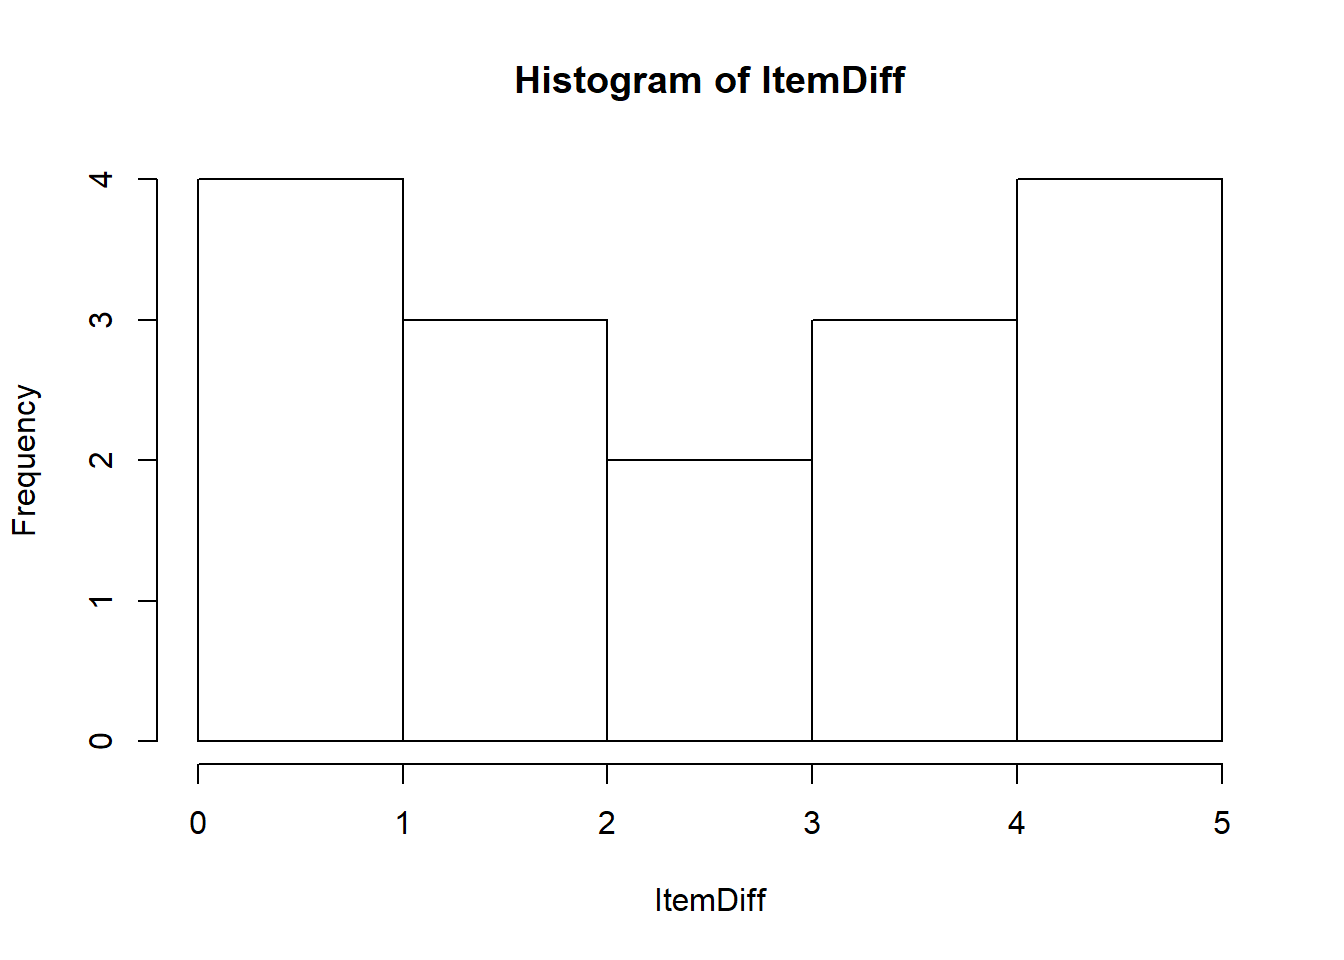
\includegraphics{Rasch_Biome_files/figure-latex/unnamed-chunk-6-1.pdf}

\hypertarget{packages-necessary-for-running-the-rasch-model}{%
\section{Packages Necessary for running the Rasch model}\label{packages-necessary-for-running-the-rasch-model}}

Install the packages below. TAM is a collection of functions to run a variety of Rasch-type models. WrightMap will help us visualize model estimated item difficulties and model estimated person abilities. We can use the Wright map to help us answer questions such as, ``do our items match our population of interest such that we have items that garner information about students at all ranges of the ability distribution?'' or ``do we have too many easy or hard items and not enough items in the middle of the ability range (are the items well targeted)?''.
Let's get into it.

If you need to install \texttt{TAM} or the \texttt{WrightMap} package, note the quotes and capitalizations:

\begin{verbatim}
install.packages("TAM")
install.packages("WrightMap")
\end{verbatim}

We need to load the packages.Additionally, we'll use some packages from the \texttt{tidyverse}

\begin{Shaded}
\begin{Highlighting}[]
\FunctionTok{library}\NormalTok{(TAM)}
\FunctionTok{library}\NormalTok{(WrightMap)}

\FunctionTok{library}\NormalTok{(tidyverse)}
\end{Highlighting}
\end{Shaded}

\hypertarget{reading-in-data}{%
\section{Reading in Data}\label{reading-in-data}}

The data for this session will be downloaded from an online repository (github). We need to read it in to your R session. This means that it is something you can now work with in R. The .csv file will be read in as something called a data frame or (dataframe). This is a type of object in R that's essentially a spreadsheet that your're used to working with.

\begin{Shaded}
\begin{Highlighting}[]
\NormalTok{hls }\OtherTok{\textless{}{-}} \FunctionTok{read\_csv}\NormalTok{(}\StringTok{"https://raw.githubusercontent.com/danielbkatz/DBER\_Rasch/master/data/dichotomous.csv"}\NormalTok{)}
\end{Highlighting}
\end{Shaded}

\begin{verbatim}
## Warning: Missing column names filled in: 'X1' [1]
\end{verbatim}

\begin{verbatim}
## Parsed with column specification:
## cols(
##   X1 = col_double(),
##   V1 = col_double(),
##   V2 = col_double(),
##   V3 = col_double(),
##   V4 = col_double(),
##   V5 = col_double(),
##   V6 = col_double(),
##   V7 = col_double(),
##   V8 = col_double(),
##   V9 = col_double(),
##   V10 = col_double(),
##   V11 = col_double(),
##   V12 = col_double(),
##   V13 = col_double(),
##   V14 = col_double(),
##   V15 = col_double()
## )
\end{verbatim}

\begin{Shaded}
\begin{Highlighting}[]
\CommentTok{\# The first column are IDs that we\textquotesingle{}ll get rid of}
\NormalTok{hls }\OtherTok{\textless{}{-}}\NormalTok{ hls[}\SpecialCharTok{{-}}\DecValTok{1}\NormalTok{]}
\end{Highlighting}
\end{Shaded}

If you would like to download the data first, and are reading it in locally,

\begin{Shaded}
\begin{Highlighting}[]
\NormalTok{hls }\OtherTok{\textless{}{-}} \FunctionTok{read.csv}\NormalTok{(}\StringTok{"data/hls\_dic\_scale.csv"}\NormalTok{)}
\end{Highlighting}
\end{Shaded}

\hypertarget{check-out-the-data-set}{%
\section{Check out the data set}\label{check-out-the-data-set}}

Let's explore \texttt{hls} just a little. It has 15 columns (the items, and 1000 rows, the people). Each item is titled ``V1\ldots vN.'' There is no missing data.

\begin{Shaded}
\begin{Highlighting}[]
\FunctionTok{dim}\NormalTok{(hls)}
\end{Highlighting}
\end{Shaded}

\begin{verbatim}
## [1] 1000   15
\end{verbatim}

\begin{Shaded}
\begin{Highlighting}[]
\FunctionTok{str}\NormalTok{(hls)}
\end{Highlighting}
\end{Shaded}

\begin{verbatim}
## tibble [1,000 x 15] (S3: tbl_df/tbl/data.frame)
##  $ V1 : num [1:1000] 0 0 0 0 1 0 0 0 0 1 ...
##  $ V2 : num [1:1000] 0 0 0 0 0 0 0 1 0 0 ...
##  $ V3 : num [1:1000] 0 0 0 0 0 0 1 1 1 0 ...
##  $ V4 : num [1:1000] 0 0 1 0 1 0 0 0 0 1 ...
##  $ V5 : num [1:1000] 0 0 0 0 1 0 0 0 0 0 ...
##  $ V6 : num [1:1000] 1 1 1 1 1 0 1 0 1 1 ...
##  $ V7 : num [1:1000] 1 1 1 0 1 1 0 1 0 1 ...
##  $ V8 : num [1:1000] 1 1 1 0 1 1 1 0 0 1 ...
##  $ V9 : num [1:1000] 1 0 1 0 0 1 1 0 0 1 ...
##  $ V10: num [1:1000] 1 1 1 1 1 1 1 1 1 1 ...
##  $ V11: num [1:1000] 0 0 0 0 1 0 1 0 0 0 ...
##  $ V12: num [1:1000] 1 1 1 0 1 0 1 0 1 1 ...
##  $ V13: num [1:1000] 1 1 1 1 1 1 1 1 1 1 ...
##  $ V14: num [1:1000] 1 1 1 1 1 1 1 0 0 0 ...
##  $ V15: num [1:1000] 1 1 1 1 1 0 1 0 0 1 ...
\end{verbatim}

\begin{Shaded}
\begin{Highlighting}[]
\FunctionTok{head}\NormalTok{(hls)}
\end{Highlighting}
\end{Shaded}

\begin{verbatim}
## # A tibble: 6 x 15
##      V1    V2    V3    V4    V5    V6    V7    V8    V9
##   <dbl> <dbl> <dbl> <dbl> <dbl> <dbl> <dbl> <dbl> <dbl>
## 1     0     0     0     0     0     1     1     1     1
## 2     0     0     0     0     0     1     1     1     0
## 3     0     0     0     1     0     1     1     1     1
## 4     0     0     0     0     0     1     0     0     0
## 5     1     0     0     1     1     1     1     1     0
## 6     0     0     0     0     0     0     1     1     1
## # ... with 6 more variables: V10 <dbl>, V11 <dbl>,
## #   V12 <dbl>, V13 <dbl>, V14 <dbl>, V15 <dbl>
\end{verbatim}

If you want to see the whole dataset, view the data frame:

\begin{Shaded}
\begin{Highlighting}[]
\FunctionTok{View}\NormalTok{(hls)}
\end{Highlighting}
\end{Shaded}

\hypertarget{running-the-rasch-model}{%
\section{Running the Rasch model}\label{running-the-rasch-model}}

This command runs a Rasch model on the selected data frame. Here, \texttt{mod1} is an object in R that ``holds'' the data from our Rasch model (along with a lot of other information). It's essentially a large list. This is the main computation step, now we just select information that is stored in \texttt{mod1} or run \texttt{mod1} through further computation.

Note that the dataframe \texttt{hls} has to contain only items and no other information.

\begin{Shaded}
\begin{Highlighting}[]
\NormalTok{mod1 }\OtherTok{\textless{}{-}} \FunctionTok{tam}\NormalTok{(hls)}
\end{Highlighting}
\end{Shaded}

\begin{verbatim}
## ....................................................
## Processing Data      2021-02-07 11:12:40 
##     * Response Data: 1000 Persons and  15 Items 
##     * Numerical integration with 21 nodes
##     * Created Design Matrices   ( 2021-02-07 11:12:40 )
##     * Calculated Sufficient Statistics   ( 2021-02-07 11:12:40 )
## ....................................................
## Iteration 1     2021-02-07 11:12:40
## E Step
## M Step Intercepts   |----
##   Deviance = 14773.234
##   Maximum item intercept parameter change: 0.399105
##   Maximum item slope parameter change: 0
##   Maximum regression parameter change: 0
##   Maximum variance parameter change: 0.078497
## ....................................................
## Iteration 2     2021-02-07 11:12:40
## E Step
## M Step Intercepts   |---
##   Deviance = 14690.1844 | Absolute change: 83.0496 | Relative change: 0.00565341
##   Maximum item intercept parameter change: 0.021879
##   Maximum item slope parameter change: 0
##   Maximum regression parameter change: 0
##   Maximum variance parameter change: 0.033763
## ....................................................
## Iteration 3     2021-02-07 11:12:40
## E Step
## M Step Intercepts   |--
##   Deviance = 14688.5292 | Absolute change: 1.6552 | Relative change: 0.00011269
##   Maximum item intercept parameter change: 0.014713
##   Maximum item slope parameter change: 0
##   Maximum regression parameter change: 0
##   Maximum variance parameter change: 0.023636
## ....................................................
## Iteration 4     2021-02-07 11:12:40
## E Step
## M Step Intercepts   |--
##   Deviance = 14687.7687 | Absolute change: 0.7605 | Relative change: 5.177e-05
##   Maximum item intercept parameter change: 0.010151
##   Maximum item slope parameter change: 0
##   Maximum regression parameter change: 0
##   Maximum variance parameter change: 0.016163
## ....................................................
## Iteration 5     2021-02-07 11:12:40
## E Step
## M Step Intercepts   |--
##   Deviance = 14687.4204 | Absolute change: 0.3483 | Relative change: 2.372e-05
##   Maximum item intercept parameter change: 0.007002
##   Maximum item slope parameter change: 0
##   Maximum regression parameter change: 0
##   Maximum variance parameter change: 0.01092
## ....................................................
## Iteration 6     2021-02-07 11:12:40
## E Step
## M Step Intercepts   |--
##   Deviance = 14687.2608 | Absolute change: 0.1595 | Relative change: 1.086e-05
##   Maximum item intercept parameter change: 0.004829
##   Maximum item slope parameter change: 0
##   Maximum regression parameter change: 0
##   Maximum variance parameter change: 0.007322
## ....................................................
## Iteration 7     2021-02-07 11:12:40
## E Step
## M Step Intercepts   |--
##   Deviance = 14687.1876 | Absolute change: 0.0733 | Relative change: 4.99e-06
##   Maximum item intercept parameter change: 0.003331
##   Maximum item slope parameter change: 0
##   Maximum regression parameter change: 0
##   Maximum variance parameter change: 0.004888
## ....................................................
## Iteration 8     2021-02-07 11:12:40
## E Step
## M Step Intercepts   |--
##   Deviance = 14687.1538 | Absolute change: 0.0338 | Relative change: 2.3e-06
##   Maximum item intercept parameter change: 0.0023
##   Maximum item slope parameter change: 0
##   Maximum regression parameter change: 0
##   Maximum variance parameter change: 0.003254
## ....................................................
## Iteration 9     2021-02-07 11:12:40
## E Step
## M Step Intercepts   |--
##   Deviance = 14687.1382 | Absolute change: 0.0156 | Relative change: 1.06e-06
##   Maximum item intercept parameter change: 0.001589
##   Maximum item slope parameter change: 0
##   Maximum regression parameter change: 0
##   Maximum variance parameter change: 0.002164
## ....................................................
## Iteration 10     2021-02-07 11:12:40
## E Step
## M Step Intercepts   |--
##   Deviance = 14687.1309 | Absolute change: 0.0073 | Relative change: 5e-07
##   Maximum item intercept parameter change: 0.001098
##   Maximum item slope parameter change: 0
##   Maximum regression parameter change: 0
##   Maximum variance parameter change: 0.001439
## ....................................................
## Iteration 11     2021-02-07 11:12:40
## E Step
## M Step Intercepts   |--
##   Deviance = 14687.1275 | Absolute change: 0.0034 | Relative change: 2.3e-07
##   Maximum item intercept parameter change: 0.00076
##   Maximum item slope parameter change: 0
##   Maximum regression parameter change: 0
##   Maximum variance parameter change: 0.000957
## ....................................................
## Iteration 12     2021-02-07 11:12:40
## E Step
## M Step Intercepts   |--
##   Deviance = 14687.1259 | Absolute change: 0.0016 | Relative change: 1.1e-07
##   Maximum item intercept parameter change: 0.000526
##   Maximum item slope parameter change: 0
##   Maximum regression parameter change: 0
##   Maximum variance parameter change: 0.000637
## ....................................................
## Iteration 13     2021-02-07 11:12:40
## E Step
## M Step Intercepts   |--
##   Deviance = 14687.1251 | Absolute change: 8e-04 | Relative change: 5e-08
##   Maximum item intercept parameter change: 0.000365
##   Maximum item slope parameter change: 0
##   Maximum regression parameter change: 0
##   Maximum variance parameter change: 0.000425
## ....................................................
## Iteration 14     2021-02-07 11:12:40
## E Step
## M Step Intercepts   |--
##   Deviance = 14687.1248 | Absolute change: 4e-04 | Relative change: 2e-08
##   Maximum item intercept parameter change: 0.000253
##   Maximum item slope parameter change: 0
##   Maximum regression parameter change: 0
##   Maximum variance parameter change: 0.000284
## ....................................................
## Iteration 15     2021-02-07 11:12:40
## E Step
## M Step Intercepts   |--
##   Deviance = 14687.1246 | Absolute change: 2e-04 | Relative change: 1e-08
##   Maximum item intercept parameter change: 0.000176
##   Maximum item slope parameter change: 0
##   Maximum regression parameter change: 0
##   Maximum variance parameter change: 0.00019
## ....................................................
## Iteration 16     2021-02-07 11:12:40
## E Step
## M Step Intercepts   |--
##   Deviance = 14687.1245 | Absolute change: 1e-04 | Relative change: 1e-08
##   Maximum item intercept parameter change: 0.000122
##   Maximum item slope parameter change: 0
##   Maximum regression parameter change: 0
##   Maximum variance parameter change: 0.000127
## ....................................................
## Iteration 17     2021-02-07 11:12:40
## E Step
## M Step Intercepts   |-
##   Deviance = 14687.1245 | Absolute change: 0 | Relative change: 0
##   Maximum item intercept parameter change: 8.5e-05
##   Maximum item slope parameter change: 0
##   Maximum regression parameter change: 0
##   Maximum variance parameter change: 8.5e-05
## ....................................................
## Item Parameters
##    xsi.index xsi.label     est
## 1          1        V1  1.7931
## 2          2        V2  2.9362
## 3          3        V3  1.8480
## 4          4        V4  1.9376
## 5          5        V5  1.1392
## 6          6        V6 -0.3249
## 7          7        V7  0.2917
## 8          8        V8  0.1005
## 9          9        V9  0.3164
## 10        10       V10 -2.7690
## 11        11       V11  2.3171
## 12        12       V12 -1.3863
## 13        13       V13 -3.1003
## 14        14       V14 -0.5554
## 15        15       V15 -0.2020
## ...................................
## Regression Coefficients
##      [,1]
## [1,]    0
## 
## Variance:
##       [,1]
## [1,] 1.028
## 
## 
## EAP Reliability:
## [1] 0.691
## 
## -----------------------------
## Start:  2021-02-07 11:12:40
## End:  2021-02-07 11:12:40 
## Time difference of 0.0849998 secs
\end{verbatim}

If we want to see some basic results from mod1, we can use \texttt{summary}

\begin{Shaded}
\begin{Highlighting}[]
\FunctionTok{summary}\NormalTok{(mod1)}
\end{Highlighting}
\end{Shaded}

\begin{verbatim}
## ------------------------------------------------------------
## TAM 3.5-19 (2020-05-05 22:45:39) 
## R version 3.6.0 (2019-04-26) x86_64, mingw32 | nodename=LAPTOP-K7402PLE | login=katzd 
## 
## Date of Analysis: 2021-02-07 11:12:40 
## Time difference of 0.0849998 secs
## Computation time: 0.0849998 
## 
## Multidimensional Item Response Model in TAM 
## 
## IRT Model: 1PL
## Call:
## tam.mml(resp = resp)
## 
## ------------------------------------------------------------
## Number of iterations = 17 
## Numeric integration with 21 integration points
## 
## Deviance = 14687.12 
## Log likelihood = -7343.56 
## Number of persons = 1000 
## Number of persons used = 1000 
## Number of items = 15 
## Number of estimated parameters = 16 
##     Item threshold parameters = 15 
##     Item slope parameters = 0 
##     Regression parameters = 0 
##     Variance/covariance parameters = 1 
## 
## AIC = 14719  | penalty=32    | AIC=-2*LL + 2*p 
## AIC3 = 14735  | penalty=48    | AIC3=-2*LL + 3*p 
## BIC = 14798  | penalty=110.52    | BIC=-2*LL + log(n)*p 
## aBIC = 14747  | penalty=59.64    | aBIC=-2*LL + log((n-2)/24)*p  (adjusted BIC) 
## CAIC = 14814  | penalty=126.52    | CAIC=-2*LL + [log(n)+1]*p  (consistent AIC) 
## AICc = 14720  | penalty=32.55    | AICc=-2*LL + 2*p + 2*p*(p+1)/(n-p-1)  (bias corrected AIC) 
## GHP = 0.49064     | GHP=( -LL + p ) / (#Persons * #Items)  (Gilula-Haberman log penalty) 
## 
## ------------------------------------------------------------
## EAP Reliability
## [1] 0.691
## ------------------------------------------------------------
## Covariances and Variances
##       [,1]
## [1,] 1.028
## ------------------------------------------------------------
## Correlations and Standard Deviations (in the diagonal)
##       [,1]
## [1,] 1.014
## ------------------------------------------------------------
## Regression Coefficients
##      [,1]
## [1,]    0
## ------------------------------------------------------------
## Item Parameters -A*Xsi
##    item    N     M xsi.item AXsi_.Cat1 B.Cat1.Dim1
## 1    V1 1000 0.182    1.793      1.793           1
## 2    V2 1000 0.074    2.936      2.936           1
## 3    V3 1000 0.175    1.848      1.848           1
## 4    V4 1000 0.164    1.938      1.938           1
## 5    V5 1000 0.280    1.139      1.139           1
## 6    V6 1000 0.566   -0.325     -0.325           1
## 7    V7 1000 0.440    0.292      0.292           1
## 8    V8 1000 0.479    0.100      0.100           1
## 9    V9 1000 0.435    0.316      0.316           1
## 10  V10 1000 0.915   -2.769     -2.769           1
## 11  V11 1000 0.123    2.317      2.317           1
## 12  V12 1000 0.760   -1.386     -1.386           1
## 13  V13 1000 0.936   -3.100     -3.100           1
## 14  V14 1000 0.612   -0.555     -0.555           1
## 15  V15 1000 0.541   -0.202     -0.202           1
## 
## Item Parameters in IRT parameterization
##    item alpha   beta
## 1    V1     1  1.793
## 2    V2     1  2.936
## 3    V3     1  1.848
## 4    V4     1  1.938
## 5    V5     1  1.139
## 6    V6     1 -0.325
## 7    V7     1  0.292
## 8    V8     1  0.100
## 9    V9     1  0.316
## 10  V10     1 -2.769
## 11  V11     1  2.317
## 12  V12     1 -1.386
## 13  V13     1 -3.100
## 14  V14     1 -0.555
## 15  V15     1 -0.202
\end{verbatim}

\hypertarget{item-difficulties}{%
\section{Item Difficulties}\label{item-difficulties}}

We'll extract difficulties (\texttt{xsi}) from the \texttt{mod1} object (\texttt{mod1} is like a large list, and we can index it like we do with vectors, dataframes, etc). List objects can be indexed with double brackets (i.e.~to get the first object in a list called \texttt{list}, then we can go with: \texttt{list{[}{[}1{]}{]}} or by name, \texttt{list{[}{[}"name"{]}{]}} or \texttt{list} name). List objects can be vectors, dataframes, arrays, or another list (among other things). In TAM, the mod1 object created involves all of these things.

We'll access item difficulties via \texttt{indexing} with the \texttt{\$}. In other words, access \texttt{mod1} and extract the object \texttt{xsi} which exists in \texttt{mod1} as a datframe.

Assign those values to an object in the environment called \texttt{diffic} using \texttt{\textless{}-}, the assignment operator, like before

\begin{Shaded}
\begin{Highlighting}[]
\NormalTok{diffic }\OtherTok{\textless{}{-}}\NormalTok{ mod1}\SpecialCharTok{$}\NormalTok{xsi}
\end{Highlighting}
\end{Shaded}

\begin{Shaded}
\begin{Highlighting}[]
\NormalTok{diffic}
\end{Highlighting}
\end{Shaded}

\begin{verbatim}
##            xsi     se.xsi
## V1   1.7931307 0.08796069
## V2   2.9362293 0.12572913
## V3   1.8480436 0.08918914
## V4   1.9375978 0.09130044
## V5   1.1392412 0.07679369
## V6  -0.3249306 0.07031216
## V7   0.2917034 0.07025640
## V8   0.1004752 0.06985392
## V9   0.3164109 0.07033607
## V10 -2.7690071 0.11837091
## V11  2.3171095 0.10185622
## V12 -1.3863076 0.08015772
## V13 -3.1003020 0.13381930
## V14 -0.5553981 0.07135170
## V15 -0.2019536 0.06998711
\end{verbatim}

In the table below, we can see the item difficulties in logits in the column \texttt{xsi} and the standard error for each item \texttt{se.xsi}. One way to think of what the standard error tells us is whether item difficulties may overlap or not.

Higher \texttt{xsi} values indicate more difficult items. For instance, item Hls9 is harder than Hls8. The values are identified by constraining the mean of item difficulties to zero.

\begin{tabular}{l|r|r}
\hline
  & xsi & se.xsi\\
\hline
V1 & 1.7931307 & 0.0879607\\
\hline
V2 & 2.9362293 & 0.1257291\\
\hline
V3 & 1.8480436 & 0.0891891\\
\hline
V4 & 1.9375978 & 0.0913004\\
\hline
V5 & 1.1392412 & 0.0767937\\
\hline
V6 & -0.3249306 & 0.0703122\\
\hline
V7 & 0.2917034 & 0.0702564\\
\hline
V8 & 0.1004752 & 0.0698539\\
\hline
V9 & 0.3164109 & 0.0703361\\
\hline
V10 & -2.7690071 & 0.1183709\\
\hline
V11 & 2.3171095 & 0.1018562\\
\hline
V12 & -1.3863076 & 0.0801577\\
\hline
V13 & -3.1003020 & 0.1338193\\
\hline
V14 & -0.5553981 & 0.0713517\\
\hline
V15 & -0.2019536 & 0.0699871\\
\hline
\end{tabular}

\hypertarget{visualize---get-item-characteristic-curves}{%
\section{Visualize - Get Item Characteristic Curves}\label{visualize---get-item-characteristic-curves}}

We may want to visualize each item characteristic curve (ICC) for each item. These plots plot the expected value (blue, smooth line) given that the data fits the Rasch model, and the observed black line (a binned solution). Each plot represents a single item. They visualize the probability of a respondent getting the item correct given their ability level. For instance, for item V1, the blue line shows that a person at 1 logit (x-axis) has something like a 30\% probability of getting the item correct (predicted).

\begin{Shaded}
\begin{Highlighting}[]
\FunctionTok{plot}\NormalTok{(mod1)}
\end{Highlighting}
\end{Shaded}

\begin{verbatim}
## Iteration in WLE/MLE estimation  1   | Maximal change  1.2824 
## Iteration in WLE/MLE estimation  2   | Maximal change  0.2808 
## Iteration in WLE/MLE estimation  3   | Maximal change  0.01 
## Iteration in WLE/MLE estimation  4   | Maximal change  0.0012 
## Iteration in WLE/MLE estimation  5   | Maximal change  1e-04 
## Iteration in WLE/MLE estimation  6   | Maximal change  0 
## ----
##  WLE Reliability= 0.666
\end{verbatim}

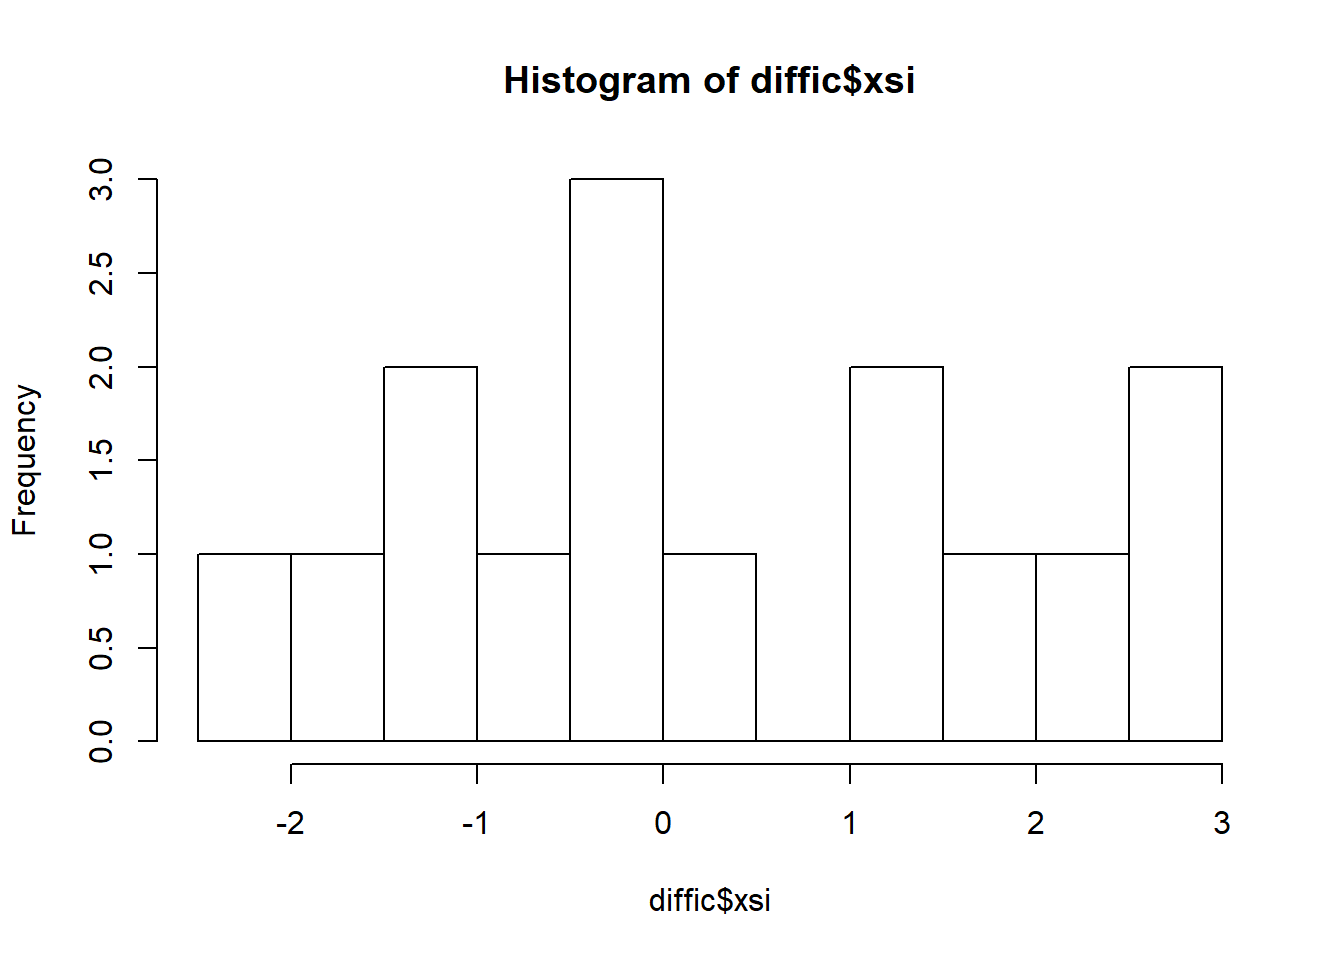
\includegraphics{Rasch_Biome_files/figure-latex/unnamed-chunk-19-1.pdf} 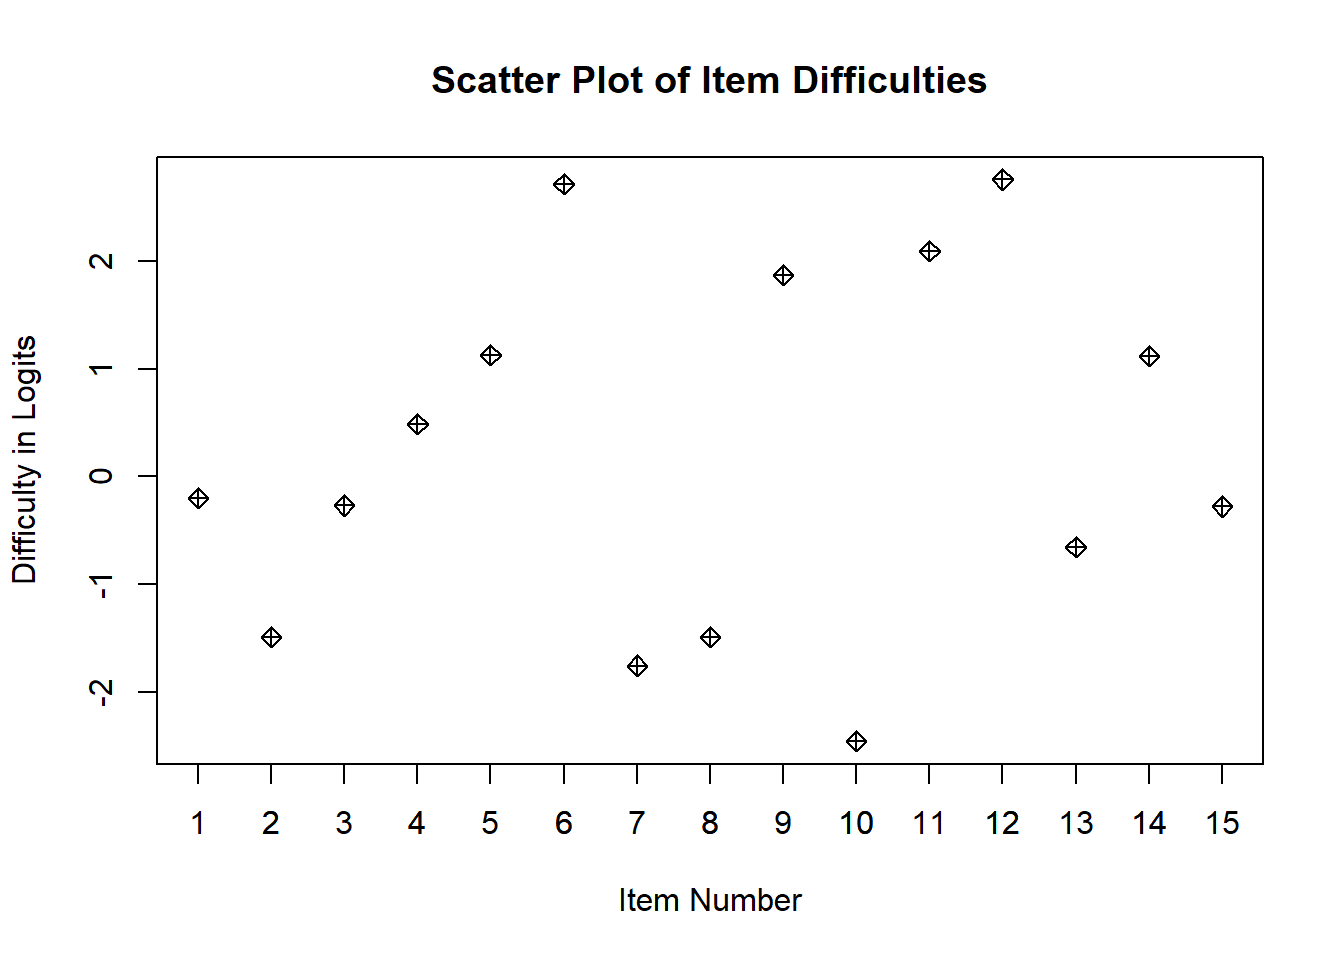
\includegraphics{Rasch_Biome_files/figure-latex/unnamed-chunk-19-2.pdf} \includegraphics{Rasch_Biome_files/figure-latex/unnamed-chunk-19-3.pdf} \includegraphics{Rasch_Biome_files/figure-latex/unnamed-chunk-19-4.pdf} \includegraphics{Rasch_Biome_files/figure-latex/unnamed-chunk-19-5.pdf} \includegraphics{Rasch_Biome_files/figure-latex/unnamed-chunk-19-6.pdf} \includegraphics{Rasch_Biome_files/figure-latex/unnamed-chunk-19-7.pdf} \includegraphics{Rasch_Biome_files/figure-latex/unnamed-chunk-19-8.pdf} \includegraphics{Rasch_Biome_files/figure-latex/unnamed-chunk-19-9.pdf} \includegraphics{Rasch_Biome_files/figure-latex/unnamed-chunk-19-10.pdf} \includegraphics{Rasch_Biome_files/figure-latex/unnamed-chunk-19-11.pdf} \includegraphics{Rasch_Biome_files/figure-latex/unnamed-chunk-19-12.pdf} \includegraphics{Rasch_Biome_files/figure-latex/unnamed-chunk-19-13.pdf} \includegraphics{Rasch_Biome_files/figure-latex/unnamed-chunk-19-14.pdf} \includegraphics{Rasch_Biome_files/figure-latex/unnamed-chunk-19-15.pdf}

\begin{verbatim}
## ....................................................
##  Plots exported in png format into folder:
##  C:/Users/katzd/Desktop/Rprojects/Rasch_BIOME/DBER_Rasch-data/Plots
\end{verbatim}

Note that for items V1 and V2, the black line, the observed probabilities, deviate quite a lot from the blue lines, the expected probabilities. Contrast this with item V5. For item V1, the black line seems to be steeper than the blue line, whereas for V2, the black line is quite a bit shallower. These lines hint at different types of item misfit, which we'll introduce later. Roughly, in the shallower case, we're not able to differentiate between respondents very easily - it probably means there is too much randomness. In the steep case, it might be too easy to differentiate - the item isn't informative.

\hypertarget{summarizing-the-distribution-of-difficulties}{%
\section{Summarizing the distribution of difficulties}\label{summarizing-the-distribution-of-difficulties}}

We can visualize and summarize the distribution of item difficulties below, but there will be a better way, called a Wright Map, that we'll introduce later.

The methods below use no packages to visualize and summarize.

\begin{Shaded}
\begin{Highlighting}[]
\FunctionTok{hist}\NormalTok{(diffic}\SpecialCharTok{$}\NormalTok{xsi, }\AttributeTok{breaks=}\DecValTok{10}\NormalTok{)}
\end{Highlighting}
\end{Shaded}

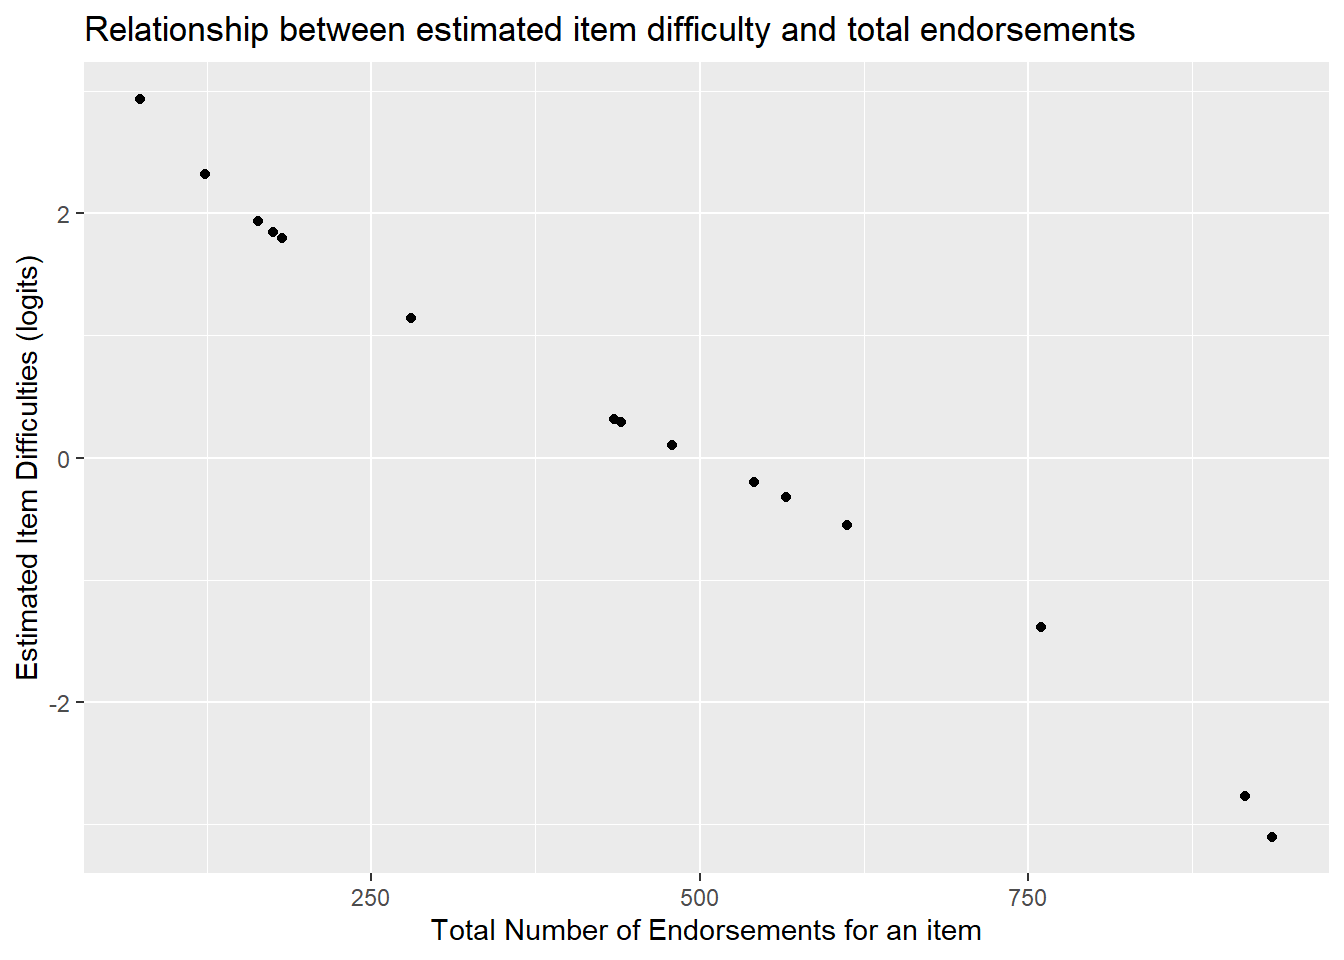
\includegraphics{Rasch_Biome_files/figure-latex/unnamed-chunk-20-1.pdf}

\begin{Shaded}
\begin{Highlighting}[]
\CommentTok{\# If you want to see the items as a scatter plot}
\FunctionTok{plot}\NormalTok{(diffic}\SpecialCharTok{$}\NormalTok{xsi, }\AttributeTok{main=}\StringTok{"Scatter Plot of Item Difficulties"}\NormalTok{, }\AttributeTok{xlab=}\StringTok{"Item Number"}\NormalTok{, }\AttributeTok{ylab =} \StringTok{"Difficulty in Logits"}\NormalTok{, }\AttributeTok{pch=}\DecValTok{9}\NormalTok{)}
\FunctionTok{axis}\NormalTok{(}\AttributeTok{side=}\DecValTok{1}\NormalTok{, }\AttributeTok{at =} \FunctionTok{c}\NormalTok{(}\DecValTok{1}\SpecialCharTok{:}\DecValTok{15}\NormalTok{))}
\end{Highlighting}
\end{Shaded}

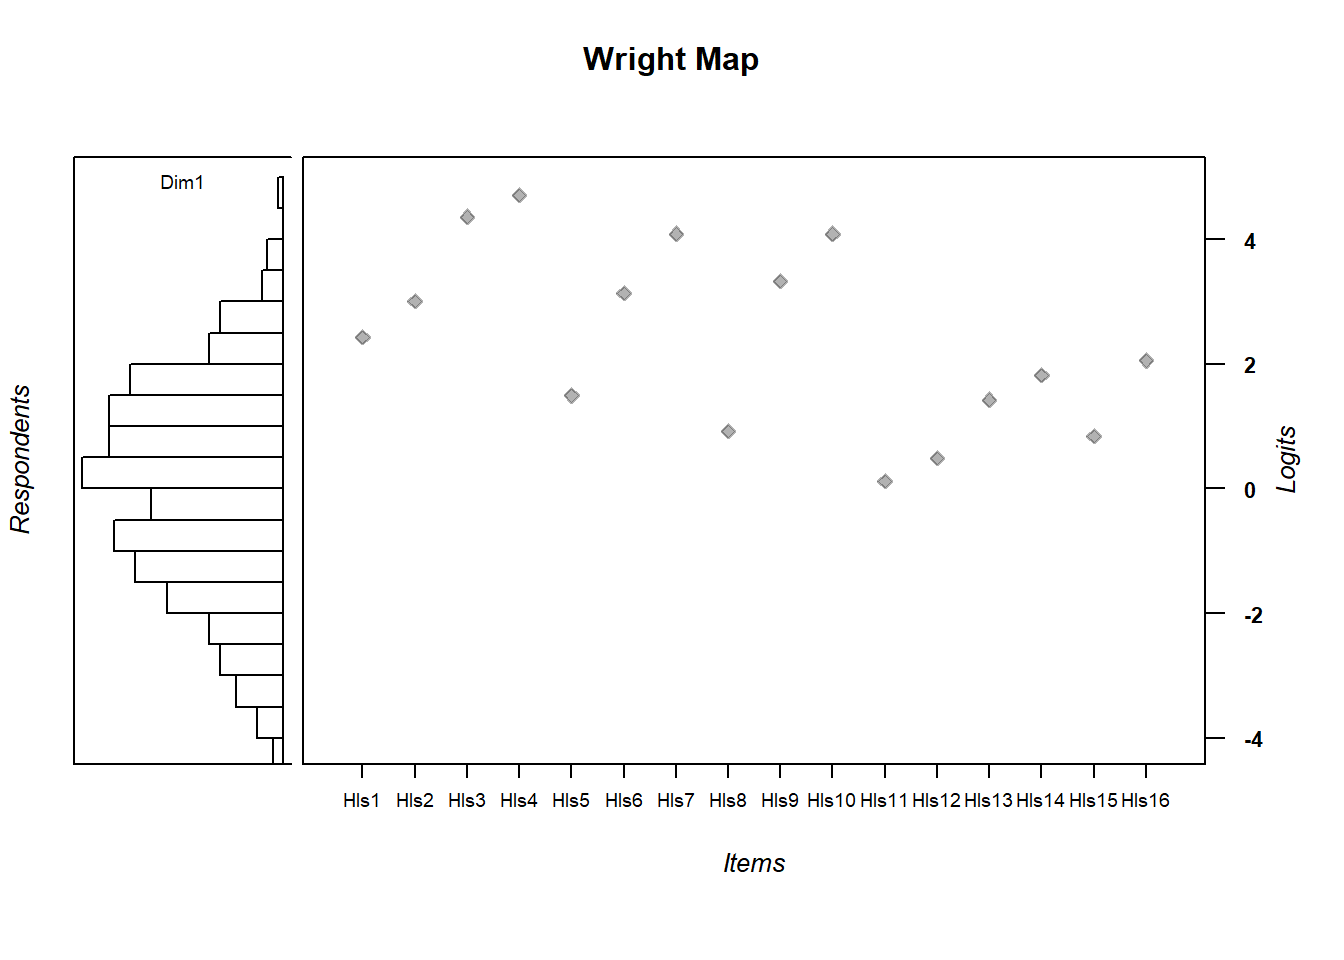
\includegraphics{Rasch_Biome_files/figure-latex/unnamed-chunk-20-2.pdf}

Let's make that difficulty plot look a bit nicer - but we can't really

\begin{Shaded}
\begin{Highlighting}[]
\CommentTok{\# create a histogram to get a sense {-} since we only have 15 items, it\textquotesingle{}s not that useful}
\FunctionTok{ggplot}\NormalTok{(diffic, }\FunctionTok{aes}\NormalTok{(}\AttributeTok{x =}\NormalTok{ xsi)) }\SpecialCharTok{+}
  \FunctionTok{geom\_histogram}\NormalTok{(}\AttributeTok{bins=}\DecValTok{15}\NormalTok{) }\SpecialCharTok{+}
  \FunctionTok{ggtitle}\NormalTok{(}\StringTok{"Distribution of Item Difficulties"}\NormalTok{)}
\end{Highlighting}
\end{Shaded}

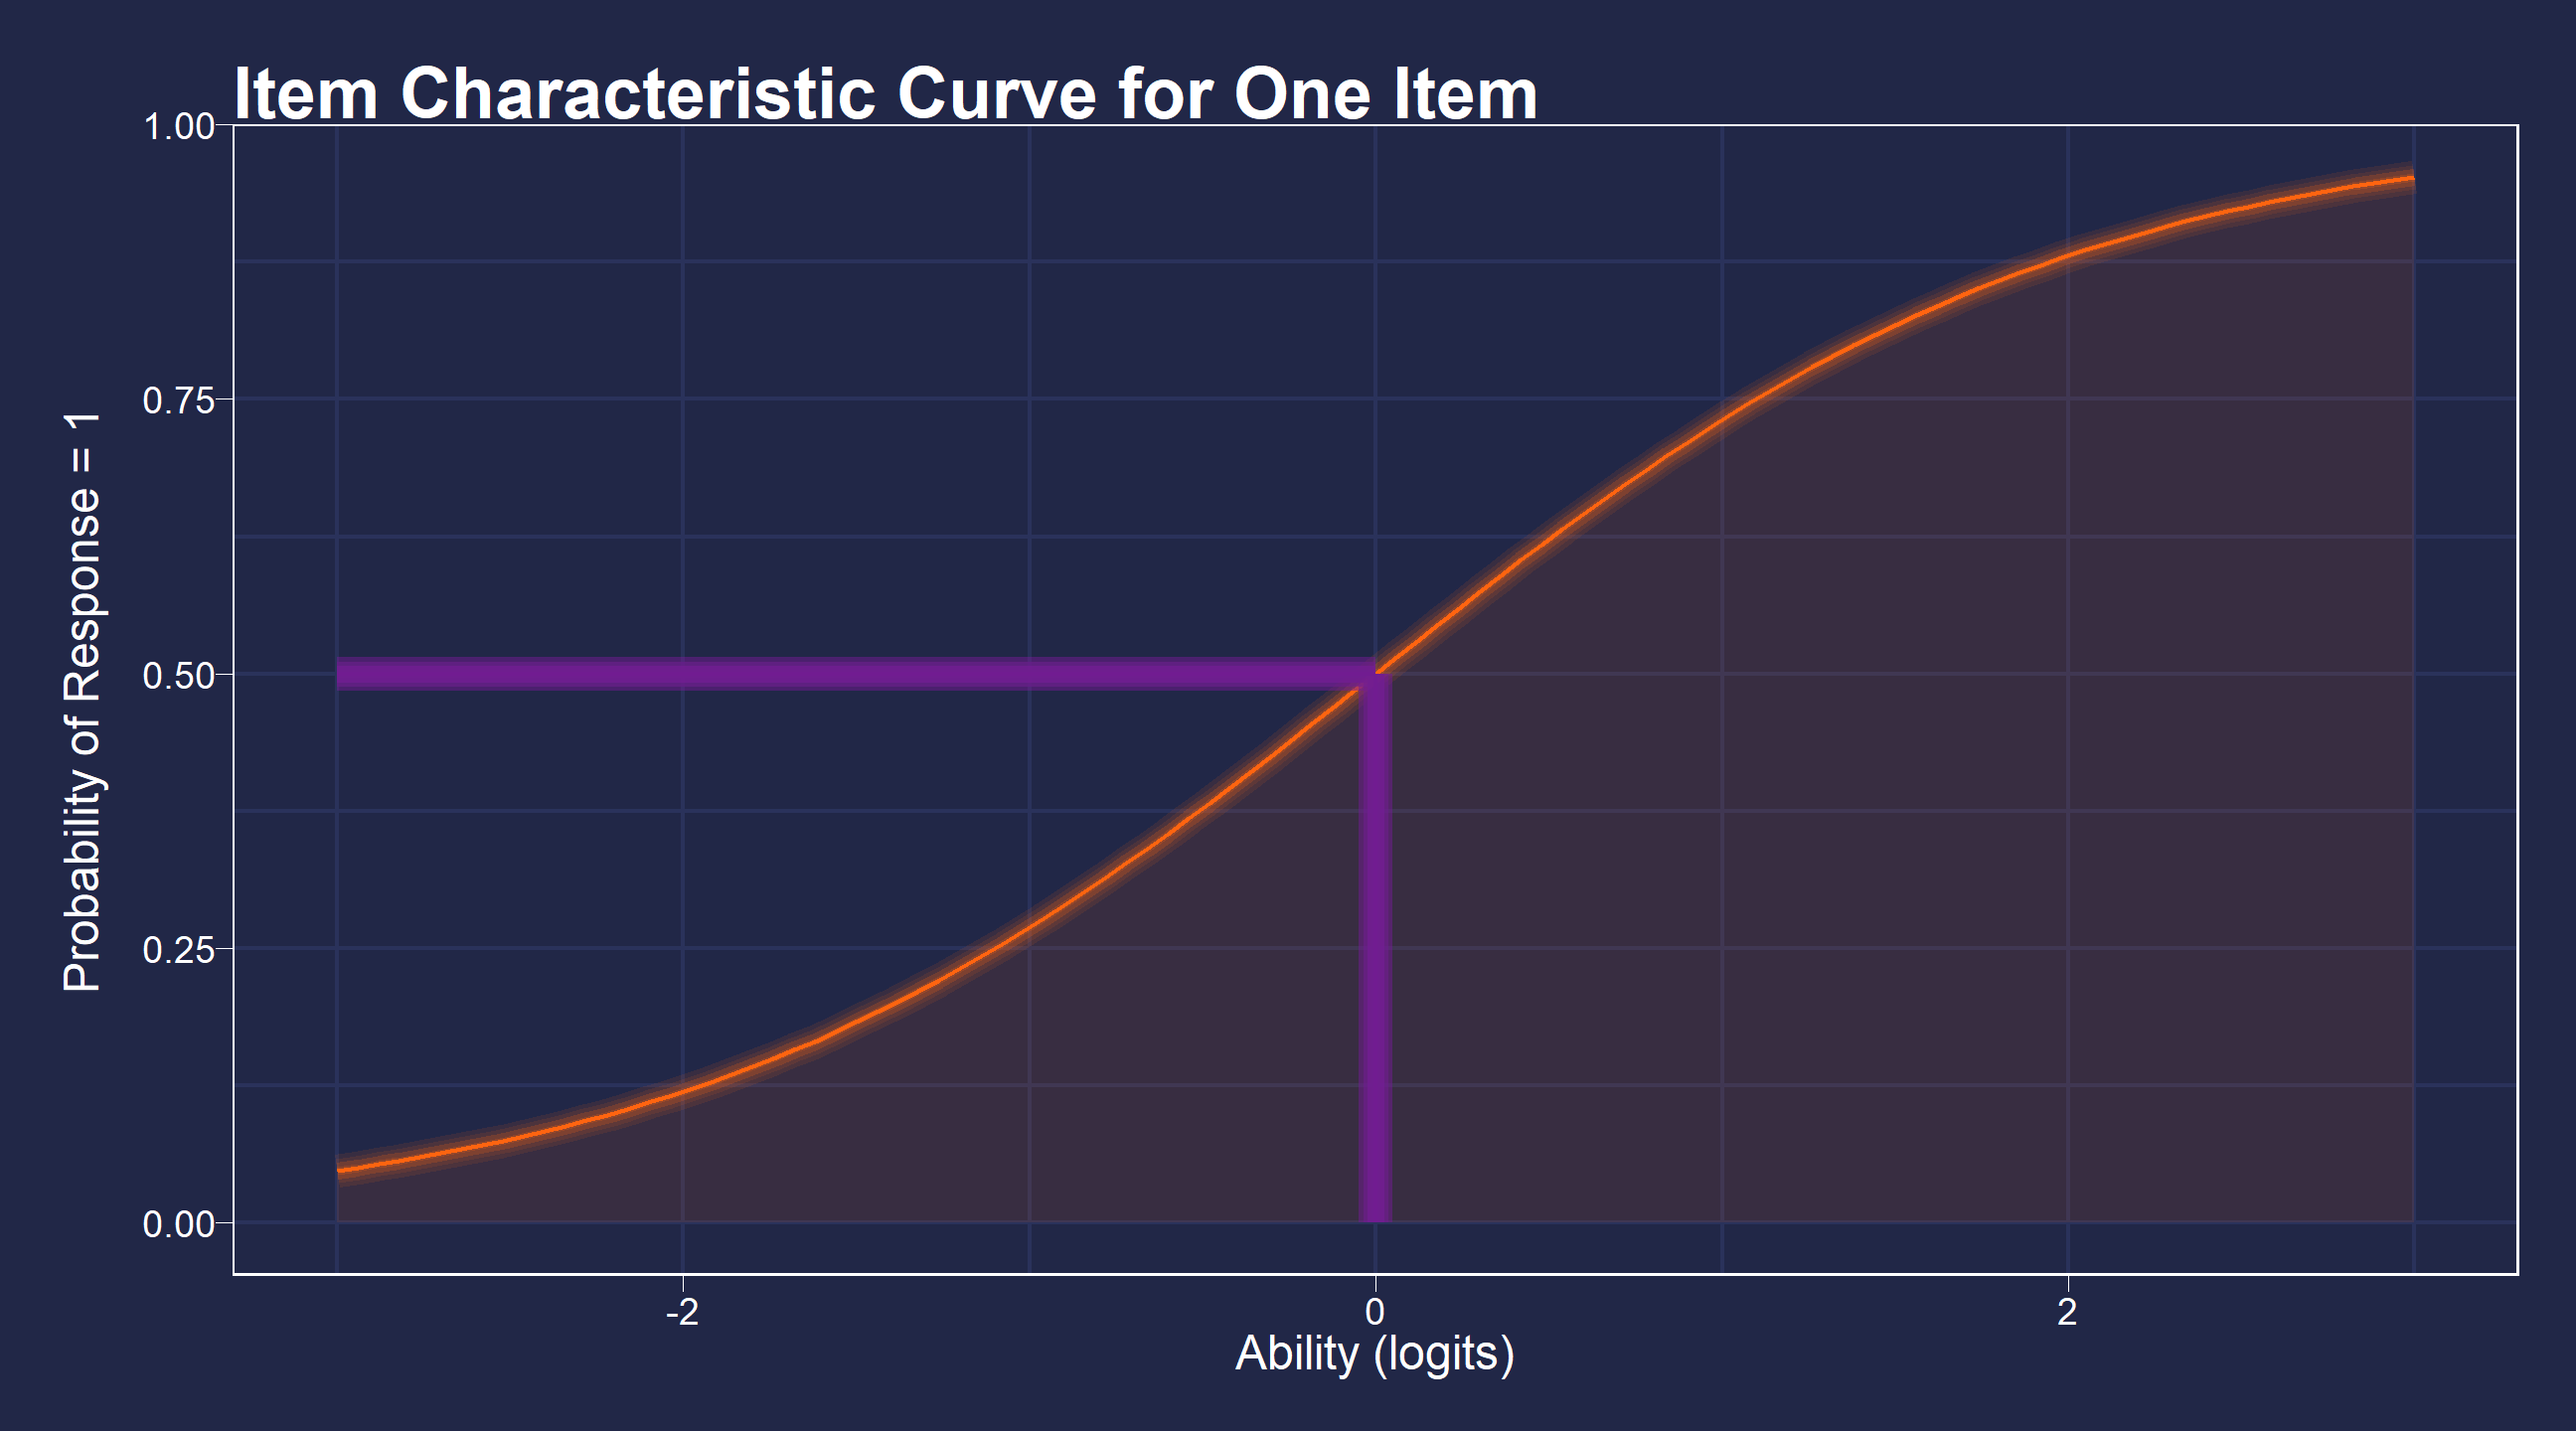
\includegraphics{Rasch_Biome_files/figure-latex/unnamed-chunk-21-1.pdf}

What might be more useful is looking at item difficulties vs their standard errors. Luckily, in this dataset, items were ordered from easiest to hardest. We see that items with larger standard errors are the hard items and the easiest items. This is because we have fewer students in the tails of the distribution - thus less information for each item - hence larger standard errors.

We'll get into this more later!

\begin{Shaded}
\begin{Highlighting}[]
\FunctionTok{ggplot}\NormalTok{(diffic, }\FunctionTok{aes}\NormalTok{(}\AttributeTok{x =}\NormalTok{ xsi, }\AttributeTok{y=}\NormalTok{se.xsi)) }\SpecialCharTok{+} \FunctionTok{geom\_point}\NormalTok{() }\SpecialCharTok{+}
  \FunctionTok{ggtitle}\NormalTok{(}\StringTok{"Item difficulties and their standard error"}\NormalTok{) }\SpecialCharTok{+}
  \FunctionTok{xlab}\NormalTok{(}\StringTok{"Estimated Item Difficulties"}\NormalTok{) }\SpecialCharTok{+}
  \FunctionTok{ylab}\NormalTok{(}\StringTok{"Estimated Item Standard Errors"}\NormalTok{)}
\end{Highlighting}
\end{Shaded}

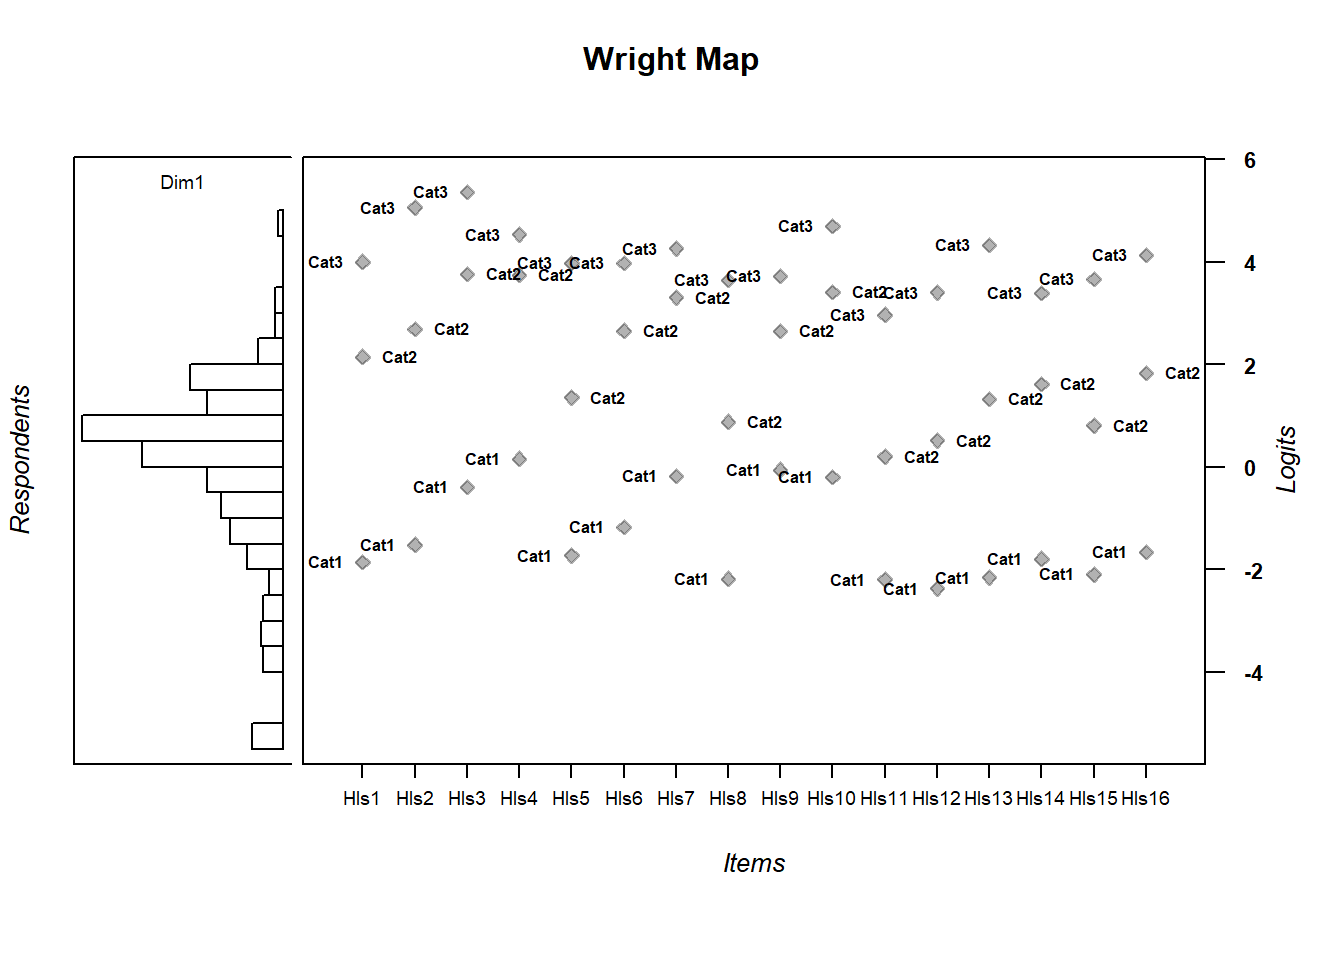
\includegraphics{Rasch_Biome_files/figure-latex/unnamed-chunk-22-1.pdf}

Another way we can get an idea of dispersion - the empirical item means and standard deviations.

\begin{Shaded}
\begin{Highlighting}[]
\FunctionTok{mean}\NormalTok{(diffic}\SpecialCharTok{$}\NormalTok{xsi)}
\end{Highlighting}
\end{Shaded}

\begin{verbatim}
## [1] 0.2894695
\end{verbatim}

\begin{Shaded}
\begin{Highlighting}[]
\FunctionTok{sd}\NormalTok{(diffic}\SpecialCharTok{$}\NormalTok{xsi)}
\end{Highlighting}
\end{Shaded}

\begin{verbatim}
## [1] 1.778192
\end{verbatim}

\hypertarget{exercise}{%
\subsection{Exercise:}\label{exercise}}

\begin{enumerate}
\def\labelenumi{\arabic{enumi}.}
\tightlist
\item
  Which item is the hardest? The easiest?
\item
  Which item has the lowest standard error - what is it's difficulty - don't use the plot.
\end{enumerate}

\hypertarget{item-fit}{%
\chapter{Item Fit}\label{item-fit}}

Let's find out if the data fit the model. Use the \texttt{tam.fit} function to compute fit statistics, then display. We note that items V1 and V2 have outfits that are drastically different from the items' infit values. We also note that infit values of V1 and V2 are different from any of the other items. We note that V1 is ``over fitting'', it's outfit and infit values being well below 1, while V2 is ``underfitting.'' This means that item V1 is too predictable - the amount of information is well predicted from other items which means it provides little new information above and beyond the other items. On the other hand, the underfitting V2 item has too much randomness.

However, outfit is ``outlier'' sensitive whereas ``infit'' is not. This implies that for V2 there might be a few responses that are particularly random/unexpected.

\begin{Shaded}
\begin{Highlighting}[]
\NormalTok{fit }\OtherTok{\textless{}{-}} \FunctionTok{tam.fit}\NormalTok{(mod1)}
\end{Highlighting}
\end{Shaded}

\begin{verbatim}
## Item fit calculation based on 15 simulations
## |**********|
## |----------|
\end{verbatim}

\begin{Shaded}
\begin{Highlighting}[]
\FunctionTok{str}\NormalTok{(fit)}
\end{Highlighting}
\end{Shaded}

\begin{verbatim}
## List of 3
##  $ itemfit:'data.frame': 15 obs. of  9 variables:
##   ..$ parameter   : Factor w/ 15 levels "V1","V10","V11",..: 1 8 9 10 11 12 13 14 15 2 ...
##   ..$ Outfit      : num [1:15] 0.633 3.691 0.992 0.936 1.066 ...
##   ..$ Outfit_t    : num [1:15] -8.304 17.04 -0.146 -1.194 1.774 ...
##   ..$ Outfit_p    : num [1:15] 1.01e-16 4.18e-65 8.84e-01 2.33e-01 7.61e-02 ...
##   ..$ Outfit_pholm: num [1:15] 1.42e-15 6.27e-64 1.00 1.00 9.89e-01 ...
##   ..$ Infit       : num [1:15] 0.83 1.234 1.029 0.961 1.044 ...
##   ..$ Infit_t     : num [1:15] -3.542 2.307 0.556 -0.7 1.21 ...
##   ..$ Infit_p     : num [1:15] 0.000398 0.021045 0.577938 0.484142 0.226153 ...
##   ..$ Infit_pholm : num [1:15] 0.00596 0.29463 1 1 1 ...
##  $ time   : POSIXct[1:2], format: "2021-02-07 11:12:58" ...
##  $ CALL   : language tam.fit(tamobj = mod1)
##  - attr(*, "class")= chr "tam.fit"
\end{verbatim}

\begin{verbatim}
View(fit$itemfit)
\end{verbatim}

\begin{tabular}{l|r|r|r|r|r|r|r|r}
\hline
parameter & Outfit & Outfit\_t & Outfit\_p & Outfit\_pholm & Infit & Infit\_t & Infit\_p & Infit\_pholm\\
\hline
V1 & 0.6334423 & -8.3035128 & 0.0000000 & 0.0000000 & 0.8296077 & -3.5416309 & 0.0003977 & 0.0059649\\
\hline
V2 & 3.6908076 & 17.0395044 & 0.0000000 & 0.0000000 & 1.2344374 & 2.3071786 & 0.0210449 & 0.2946281\\
\hline
V3 & 0.9922802 & -0.1457243 & 0.8841390 & 1.0000000 & 1.0291488 & 0.5563990 & 0.5779381 & 1.0000000\\
\hline
V4 & 0.9361118 & -1.1936740 & 0.2326055 & 1.0000000 & 0.9611833 & -0.6996561 & 0.4841421 & 1.0000000\\
\hline
V5 & 1.0659920 & 1.7737104 & 0.0761111 & 0.9894438 & 1.0443288 & 1.2103292 & 0.2261526 & 1.0000000\\
\hline
V6 & 1.0057717 & 0.2138606 & 0.8306557 & 1.0000000 & 1.0077244 & 0.2858183 & 0.7750173 & 1.0000000\\
\hline
V7 & 0.9622463 & -1.4338036 & 0.1516283 & 1.0000000 & 0.9756257 & -0.9141236 & 0.3606519 & 1.0000000\\
\hline
V8 & 0.9815854 & -0.7103794 & 0.4774689 & 1.0000000 & 0.9829529 & -0.6513461 & 0.5148231 & 1.0000000\\
\hline
V9 & 0.9748958 & -0.9417157 & 0.3463382 & 1.0000000 & 0.9748630 & -0.9371712 & 0.3486705 & 1.0000000\\
\hline
V10 & 0.9932957 & -0.0682033 & 0.9456238 & 1.0000000 & 0.9984976 & 0.0068145 & 0.9945629 & 1.0000000\\
\hline
V11 & 0.9659207 & -0.4933746 & 0.6217479 & 1.0000000 & 0.9918168 & -0.1021305 & 0.9186531 & 1.0000000\\
\hline
V12 & 1.0334256 & 0.8125654 & 0.4164673 & 1.0000000 & 1.0148597 & 0.3705174 & 0.7109970 & 1.0000000\\
\hline
V13 & 0.8752542 & -1.2275968 & 0.2195984 & 1.0000000 & 0.9998832 & 0.0298366 & 0.9761974 & 1.0000000\\
\hline
V14 & 0.9655750 & -1.2312806 & 0.2182179 & 1.0000000 & 0.9784746 & -0.7612617 & 0.4465008 & 1.0000000\\
\hline
V15 & 0.9790097 & -0.8142304 & 0.4155129 & 1.0000000 & 0.9818099 & -0.6967933 & 0.4859321 & 1.0000000\\
\hline
\end{tabular}

\hypertarget{exercise-1}{%
\subsection{Exercise:}\label{exercise-1}}

\begin{enumerate}
\def\labelenumi{\arabic{enumi}.}
\tightlist
\item
  Which items fit best? Which items fit worst?
\item
  How many, if any items, are outside the traditional bounds of mean-square item fit {[}.75, 1.33{]}?
\end{enumerate}

\hypertarget{optional---visualizing-item-fit}{%
\section{Optional - Visualizing Item Fit}\label{optional---visualizing-item-fit}}

If you'd like, we can use default \texttt{WrightMap} functionality to plot item fit statistics. In the \texttt{fit} object, \texttt{itemfit} is a dataframe containing various fit statistics. We'll plot infit with a lowerbound of .75 (in mean-square error units) and an upper bound of 1.33

The nice thing is that you can create unique fitbounds for each item (such that it's sensitive to sample size). However, if we want all the same fit values, we have to just repeat the fit value (in our case, there are 15 items).

\begin{Shaded}
\begin{Highlighting}[]
\NormalTok{infit }\OtherTok{\textless{}{-}}\NormalTok{ fit}\SpecialCharTok{$}\NormalTok{itemfit}\SpecialCharTok{$}\NormalTok{Infit}

\NormalTok{upper\_bound }\OtherTok{\textless{}{-}} \FunctionTok{rep}\NormalTok{(}\AttributeTok{x =} \FloatTok{1.33}\NormalTok{, }\AttributeTok{times =}\DecValTok{15}\NormalTok{) }\CommentTok{\# this repeats 1.33 fifteen times}
\NormalTok{lower\_bound }\OtherTok{\textless{}{-}} \FunctionTok{rep}\NormalTok{(}\AttributeTok{x =}\NormalTok{ .}\DecValTok{75}\NormalTok{, }\AttributeTok{times =} \DecValTok{15}\NormalTok{) }

\CommentTok{\# running fitgraph}


\FunctionTok{fitgraph}\NormalTok{(}\AttributeTok{fitEst =}\NormalTok{ infit, }\AttributeTok{fitLB =}\NormalTok{ lower\_bound, }\AttributeTok{fitUB =}\NormalTok{ upper\_bound, }\AttributeTok{itemLabels =} \FunctionTok{names}\NormalTok{(hls))}
\end{Highlighting}
\end{Shaded}

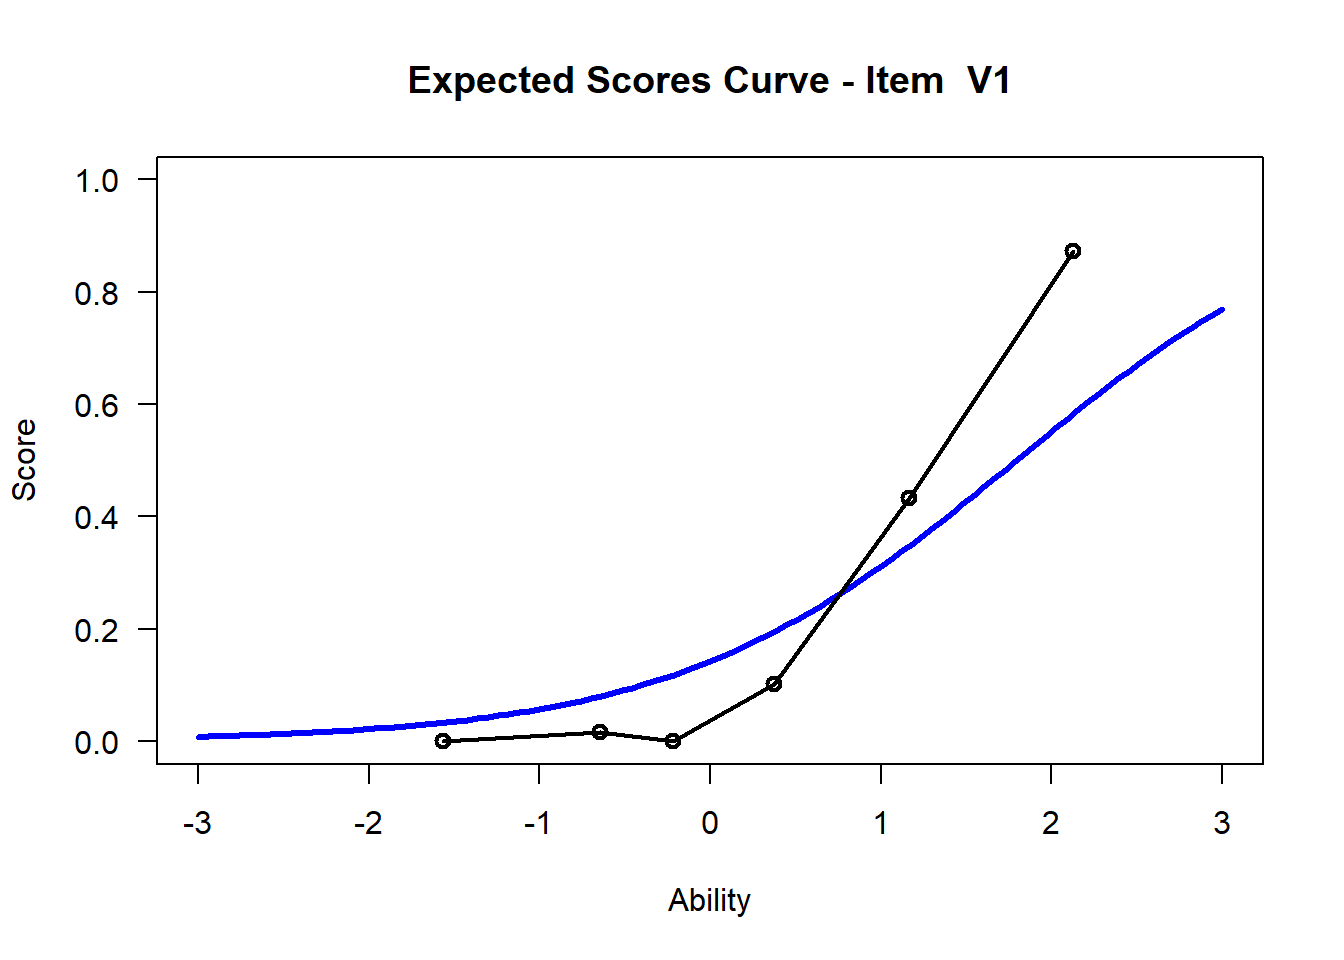
\includegraphics{Rasch_Biome_files/figure-latex/unnamed-chunk-26-1.pdf}

\begin{Shaded}
\begin{Highlighting}[]
\CommentTok{\# what about outfit?}
\NormalTok{outfit }\OtherTok{\textless{}{-}}\NormalTok{ fit}\SpecialCharTok{$}\NormalTok{itemfit}\SpecialCharTok{$}\NormalTok{Outfit}


\FunctionTok{fitgraph}\NormalTok{(}\AttributeTok{fitEst =}\NormalTok{ outfit, }\AttributeTok{fitLB =}\NormalTok{ lower\_bound, }\AttributeTok{fitUB =}\NormalTok{ upper\_bound, }\AttributeTok{itemLabels =} \FunctionTok{names}\NormalTok{(hls))}
\end{Highlighting}
\end{Shaded}

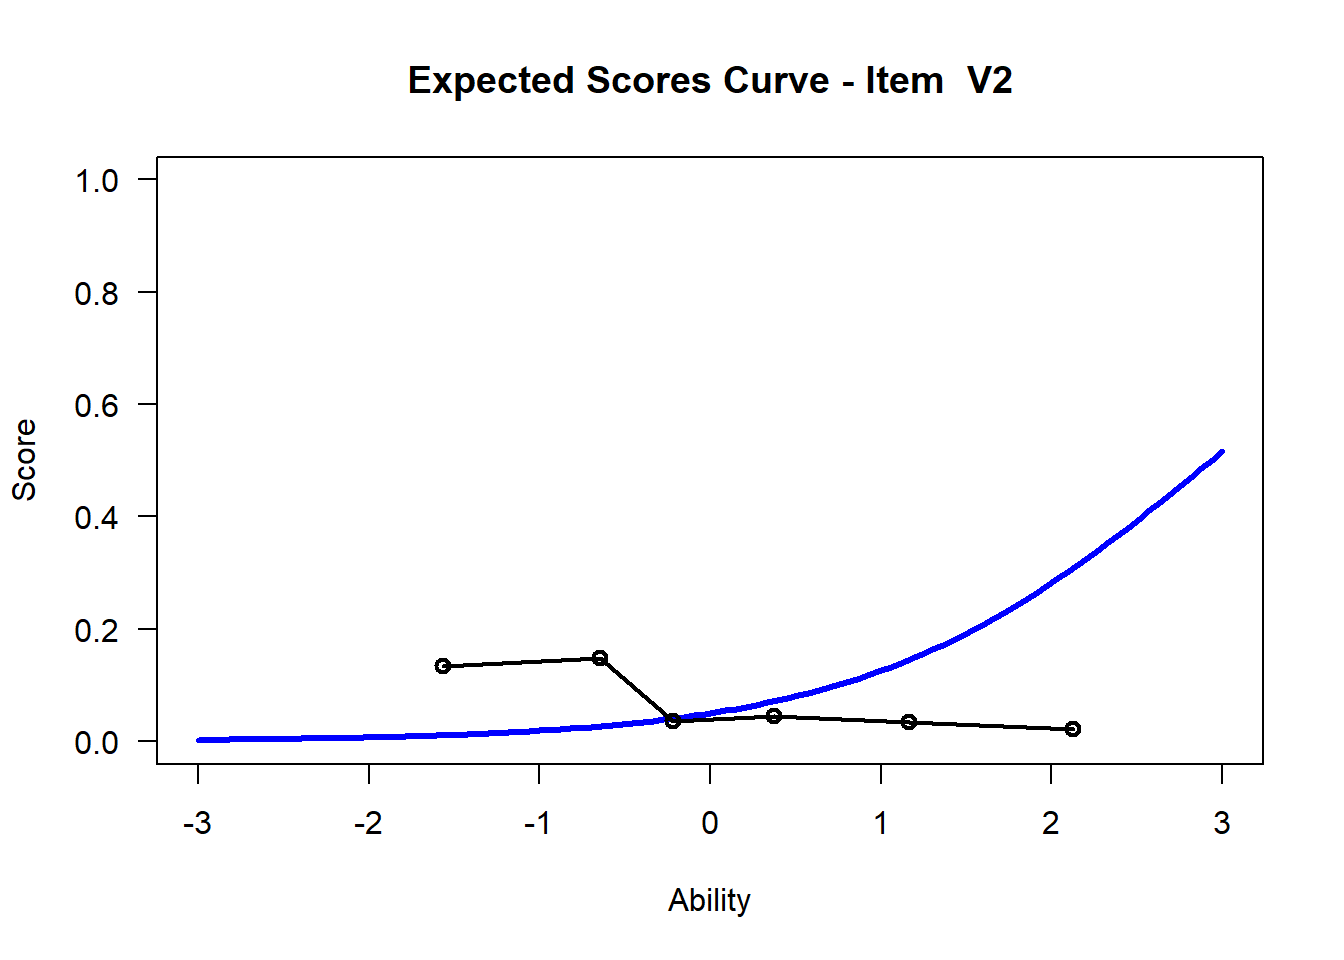
\includegraphics{Rasch_Biome_files/figure-latex/unnamed-chunk-26-2.pdf}
If you wanted to do this with ggplot - play with the code to try to change the fit limits or plot outfit instead of infit.

\begin{Shaded}
\begin{Highlighting}[]
\CommentTok{\# put the fit data in a dataframe}
\NormalTok{fit\_stats }\OtherTok{\textless{}{-}}\NormalTok{ fit}\SpecialCharTok{$}\NormalTok{itemfit}

\NormalTok{fit\_stats }\SpecialCharTok{\%\textgreater{}\%}
  \FunctionTok{ggplot}\NormalTok{(}\FunctionTok{aes}\NormalTok{(}\AttributeTok{x=}\NormalTok{parameter, }\AttributeTok{y =}\NormalTok{ infit)) }\SpecialCharTok{+} 
  \FunctionTok{geom\_point}\NormalTok{() }\SpecialCharTok{+} 
  \FunctionTok{geom\_hline}\NormalTok{(}\AttributeTok{yintercept =} \FloatTok{1.2}\NormalTok{) }\SpecialCharTok{+}
  \FunctionTok{geom\_hline}\NormalTok{(}\AttributeTok{yintercept =}\NormalTok{ .}\DecValTok{8}\NormalTok{) }\SpecialCharTok{+}
  \FunctionTok{scale\_y\_continuous}\NormalTok{(}\AttributeTok{breaks =}\NormalTok{ scales}\SpecialCharTok{::}\FunctionTok{pretty\_breaks}\NormalTok{(}\AttributeTok{n =} \DecValTok{15}\NormalTok{)) }\SpecialCharTok{+} 
  \FunctionTok{ggtitle}\NormalTok{(}\StringTok{"Item Fit Statistics for Lab 3 Data"}\NormalTok{)}
\end{Highlighting}
\end{Shaded}

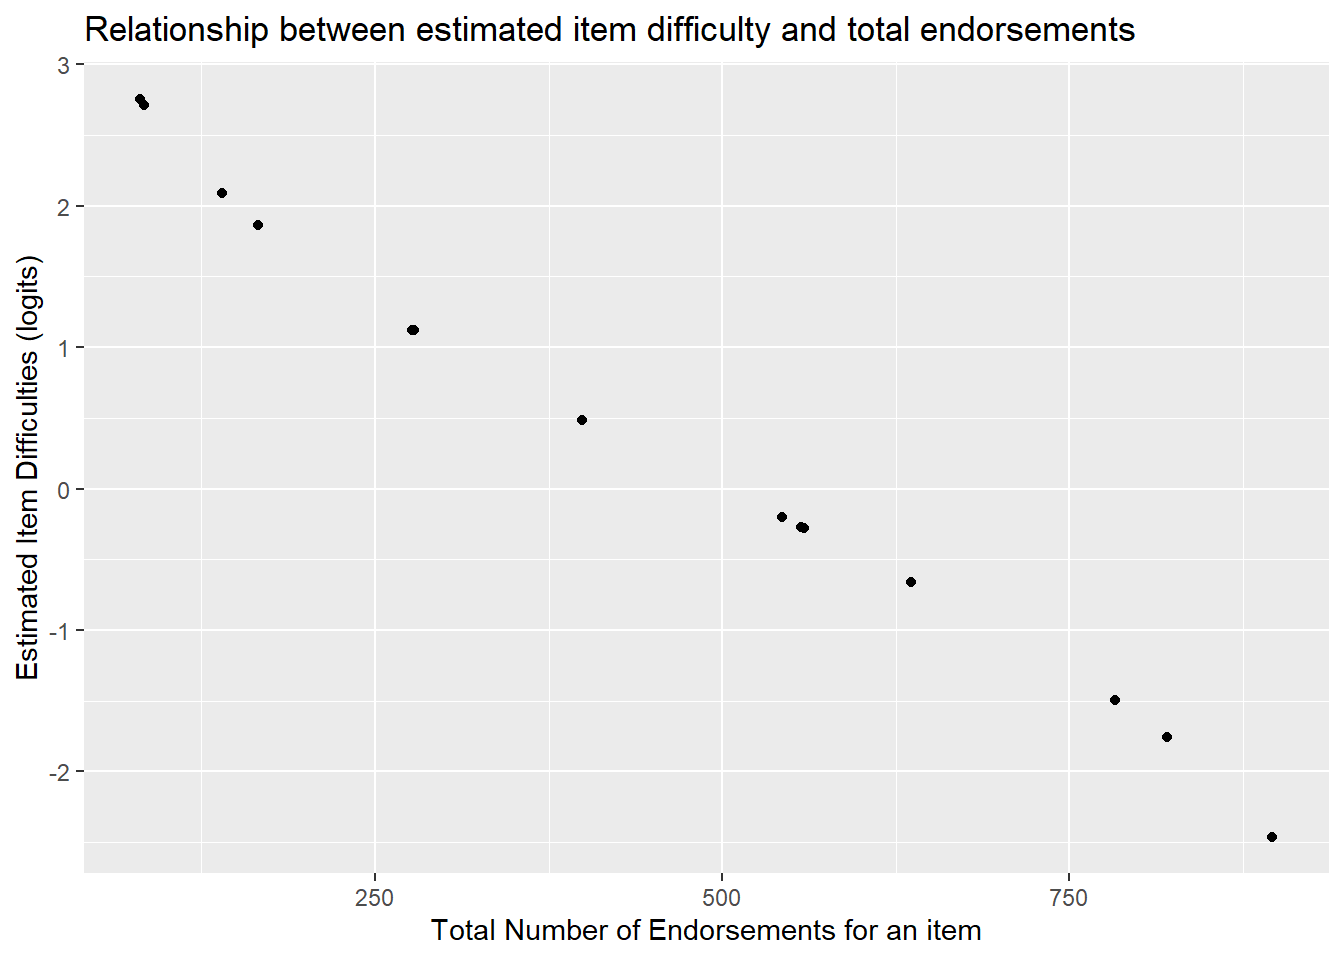
\includegraphics{Rasch_Biome_files/figure-latex/unnamed-chunk-27-1.pdf}

\hypertarget{optional-understanding-the-model}{%
\chapter{Optional: Understanding the model}\label{optional-understanding-the-model}}

\texttt{TAM} also provides some descriptive statistics.

\begin{Shaded}
\begin{Highlighting}[]
\NormalTok{item\_prop }\OtherTok{\textless{}{-}}\NormalTok{ mod1}\SpecialCharTok{$}\NormalTok{item}
\end{Highlighting}
\end{Shaded}

\begin{verbatim}
item_prop
\end{verbatim}

\begin{tabular}{l|l|r|r|r|r|r}
\hline
  & item & N & M & xsi.item & AXsi\_.Cat1 & B.Cat1.Dim1\\
\hline
V1 & V1 & 1000 & 0.182 & 1.7930554 & 1.7930554 & 1\\
\hline
V2 & V2 & 1000 & 0.074 & 2.9361446 & 2.9361446 & 1\\
\hline
V3 & V3 & 1000 & 0.175 & 1.8479678 & 1.8479678 & 1\\
\hline
V4 & V4 & 1000 & 0.164 & 1.9375212 & 1.9375212 & 1\\
\hline
V5 & V5 & 1000 & 0.280 & 1.1391729 & 1.1391729 & 1\\
\hline
V6 & V6 & 1000 & 0.566 & -0.3249806 & -0.3249806 & 1\\
\hline
V7 & V7 & 1000 & 0.440 & 0.2916454 & 0.2916454 & 1\\
\hline
V8 & V8 & 1000 & 0.479 & 0.1004197 & 0.1004197 & 1\\
\hline
V9 & V9 & 1000 & 0.435 & 0.3163527 & 0.3163527 & 1\\
\hline
V10 & V10 & 1000 & 0.915 & -2.7690302 & -2.7690302 & 1\\
\hline
V11 & V11 & 1000 & 0.123 & 2.3170294 & 2.3170294 & 1\\
\hline
V12 & V12 & 1000 & 0.760 & -1.3863445 & -1.3863445 & 1\\
\hline
V13 & V13 & 1000 & 0.936 & -3.1003226 & -3.1003226 & 1\\
\hline
V14 & V14 & 1000 & 0.612 & -0.5554452 & -0.5554452 & 1\\
\hline
V15 & V15 & 1000 & 0.541 & -0.2020052 & -0.2020052 & 1\\
\hline
\end{tabular}

Note, the total number of people who answered an item correctly is a \texttt{sufficient} statistic for calculating an item's difficulty. Said another way, the number of correct answers, or, number of people who endorse a category increases monotonically with the item difficulty (of course, this does not mean you can just replace the Rasch model with a sum score since we're using the Rasch model to test whether summing items at all is a reasonable thing to do).

To see this, we can find the total number of people who endorsed the ``agree'' category for each \texttt{Hls} item above. The table provides the proportion who endorsed the higher category in the \texttt{M} column. For instance, item Hls1 had 15.77\% of people endorse the ``agree'' category (1= agree, 0= disagree). In the N column, we see that 317 people answered the item in total.

That means that \(317*.1577\) = 50 people answering the item correctly. Note, the estimated difficulty found in the column is 2.43 logits.

\begin{Shaded}
\begin{Highlighting}[]
\CommentTok{\# Confirm that the total number of endorsements (coded 1) is 50 for Hls1: sum down the column containing all answers to Hls1 in the raw data.}


\FunctionTok{apply}\NormalTok{(hls[}\DecValTok{1}\NormalTok{], }\DecValTok{2}\NormalTok{, sum)}
\end{Highlighting}
\end{Shaded}

\begin{verbatim}
##  V1 
## 182
\end{verbatim}

However, we see that for item Hls5, 27\% of people endorsed that item and the estimated mean item difficulty in \texttt{xsi.item} is 1.50 logits.

The correlation between total number of endorsements per item and the estimated item difficulty can be computed as follows.

\begin{Shaded}
\begin{Highlighting}[]
\CommentTok{\# create a column in the item\_prop object that has the total number of endorsements for each item}
\NormalTok{item\_prop }\OtherTok{\textless{}{-}} \FunctionTok{mutate}\NormalTok{(item\_prop, }\AttributeTok{total\_endorsed =}\NormalTok{N}\SpecialCharTok{*}\NormalTok{M)}

\FunctionTok{cor}\NormalTok{(item\_prop}\SpecialCharTok{$}\NormalTok{xsi.item, item\_prop}\SpecialCharTok{$}\NormalTok{total\_endorsed)}
\end{Highlighting}
\end{Shaded}

\begin{verbatim}
## [1] -0.994751
\end{verbatim}

We see that the correlation between item difficulties and total endorsements per item is nearly perfect -.97. As the number of endorsements go down, the estimated difficulty of the item increase.

\begin{Shaded}
\begin{Highlighting}[]
\FunctionTok{ggplot}\NormalTok{(item\_prop, }\FunctionTok{aes}\NormalTok{(}\AttributeTok{x=}\NormalTok{total\_endorsed, }\AttributeTok{y=}\NormalTok{xsi.item)) }\SpecialCharTok{+} 
  \FunctionTok{geom\_point}\NormalTok{() }\SpecialCharTok{+}
  \FunctionTok{ylab}\NormalTok{(}\StringTok{"Estimated Item Difficulties (logits)"}\NormalTok{) }\SpecialCharTok{+}
  \FunctionTok{xlab}\NormalTok{(}\StringTok{"Total Number of Endorsements for an item"}\NormalTok{) }\SpecialCharTok{+}
  \FunctionTok{ggtitle}\NormalTok{(}\StringTok{"Relationship between estimated item difficulty and total endorsements"}\NormalTok{)}
\end{Highlighting}
\end{Shaded}

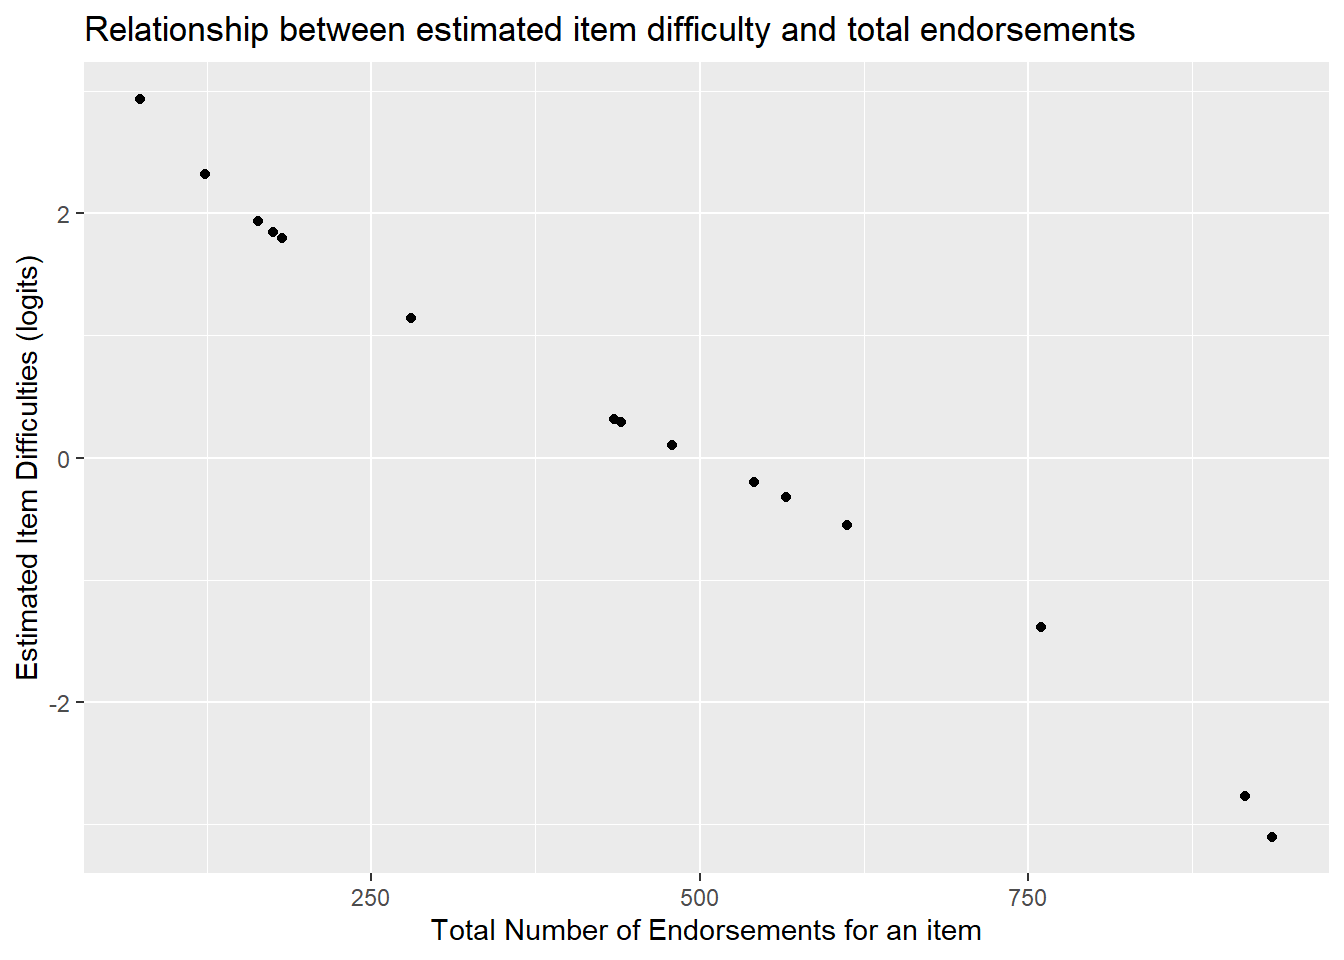
\includegraphics{Rasch_Biome_files/figure-latex/unnamed-chunk-32-1.pdf}

\hypertarget{person-abilities}{%
\chapter{Person Abilities}\label{person-abilities}}

Person abilities are also of interest. We can look at the person side of the model by computing person abilities.

\begin{enumerate}
\def\labelenumi{\arabic{enumi}.}
\item
  Compute person abilities using the \texttt{tam.wle} function and assign to an object called \texttt{abil}.
\item
  Extract person abilities (\(\theta_p\)) from \texttt{abil} to create an object in the \texttt{environment} called \texttt{PersonAbility} which will essentially be a column vector.
\end{enumerate}

\textbf{Note}: You may want more information than this at times (such as standard errors) so you may not always want to subset this way.

\begin{Shaded}
\begin{Highlighting}[]
\CommentTok{\#generates a data frame {-} output related to estimation}
\NormalTok{abil }\OtherTok{\textless{}{-}} \FunctionTok{tam.wle}\NormalTok{(mod1)}
\end{Highlighting}
\end{Shaded}

\begin{verbatim}
## Iteration in WLE/MLE estimation  1   | Maximal change  1.2824 
## Iteration in WLE/MLE estimation  2   | Maximal change  0.2808 
## Iteration in WLE/MLE estimation  3   | Maximal change  0.01 
## Iteration in WLE/MLE estimation  4   | Maximal change  0.0012 
## Iteration in WLE/MLE estimation  5   | Maximal change  1e-04 
## Iteration in WLE/MLE estimation  6   | Maximal change  0 
## ----
##  WLE Reliability= 0.666
\end{verbatim}

See the first few rows of Abil. Notice you get:

\begin{enumerate}
\def\labelenumi{\arabic{enumi}.}
\tightlist
\item
  \texttt{pid}: person id assigned by TAM.
\item
  \texttt{N.items}: Number of items the person was given (this becomes interesting when you have linked test forms where students may not all see the same number of items)
\item
  \texttt{PersonScores}: Number of items the student got right or endorsed (in the survey case).
\item
  \texttt{PersonMax}: Max total that person could have gotten right/selected an option for
\item
  \texttt{theta}: estimated person ability
\item
  \texttt{error}: estimated measurement error
\item
  \texttt{WLE.rel}: estimated person seperation reliability.
\end{enumerate}

\begin{verbatim}
head(Abil)

# or

View(Abil)
\end{verbatim}

\begin{tabular}{r|r|r|r|r|r|r}
\hline
pid & N.items & PersonScores & PersonMax & theta & error & WLE.rel\\
\hline
1 & 15 & 9 & 15 & 0.9846072 & 0.6445392 & 0.666301\\
\hline
2 & 15 & 8 & 15 & 0.5861029 & 0.6396378 & 0.666301\\
\hline
3 & 15 & 10 & 15 & 1.3941069 & 0.6580203 & 0.666301\\
\hline
4 & 15 & 5 & 15 & -0.6435504 & 0.6827321 & 0.666301\\
\hline
5 & 15 & 12 & 15 & 2.2922517 & 0.7261986 & 0.666301\\
\hline
6 & 15 & 6 & 15 & -0.2146746 & 0.6565507 & 0.666301\\
\hline
\end{tabular}

The column in the \texttt{abil} data.frame corresponding to person estimates is the \texttt{theta} column. Pull out the ability estimates, theta, column if you would like, though, this creates a list. This makes it a little easier for a few basic tasks below.

\begin{Shaded}
\begin{Highlighting}[]
\NormalTok{PersonAbility }\OtherTok{\textless{}{-}}\NormalTok{ abil}\SpecialCharTok{$}\NormalTok{theta}
\end{Highlighting}
\end{Shaded}

\begin{Shaded}
\begin{Highlighting}[]
\CommentTok{\# Only the first 6 rows, shown}
\FunctionTok{head}\NormalTok{(PersonAbility)}
\end{Highlighting}
\end{Shaded}

\begin{verbatim}
## [1]  0.9846072  0.5861029  1.3941069 -0.6435504  2.2922517
## [6] -0.2146746
\end{verbatim}

You can export those estimated abilites to a .csv to save (you can also save directly in R, if you need to). This writes \texttt{abil} as a csv file to your \texttt{output} directory that we created earlier using the \texttt{here} package.

\begin{verbatim}
write.csv(abil, here("output", "HLSmod1_thetas.csv")
\end{verbatim}

\hypertarget{quick-descriptives-for-person-ability---well-use-wrightmap-to-bring-this-all-together}{%
\section{Quick descriptives for person ability - we'll use WrightMap to bring this all together}\label{quick-descriptives-for-person-ability---well-use-wrightmap-to-bring-this-all-together}}

\begin{Shaded}
\begin{Highlighting}[]
\FunctionTok{hist}\NormalTok{(PersonAbility)}
\end{Highlighting}
\end{Shaded}

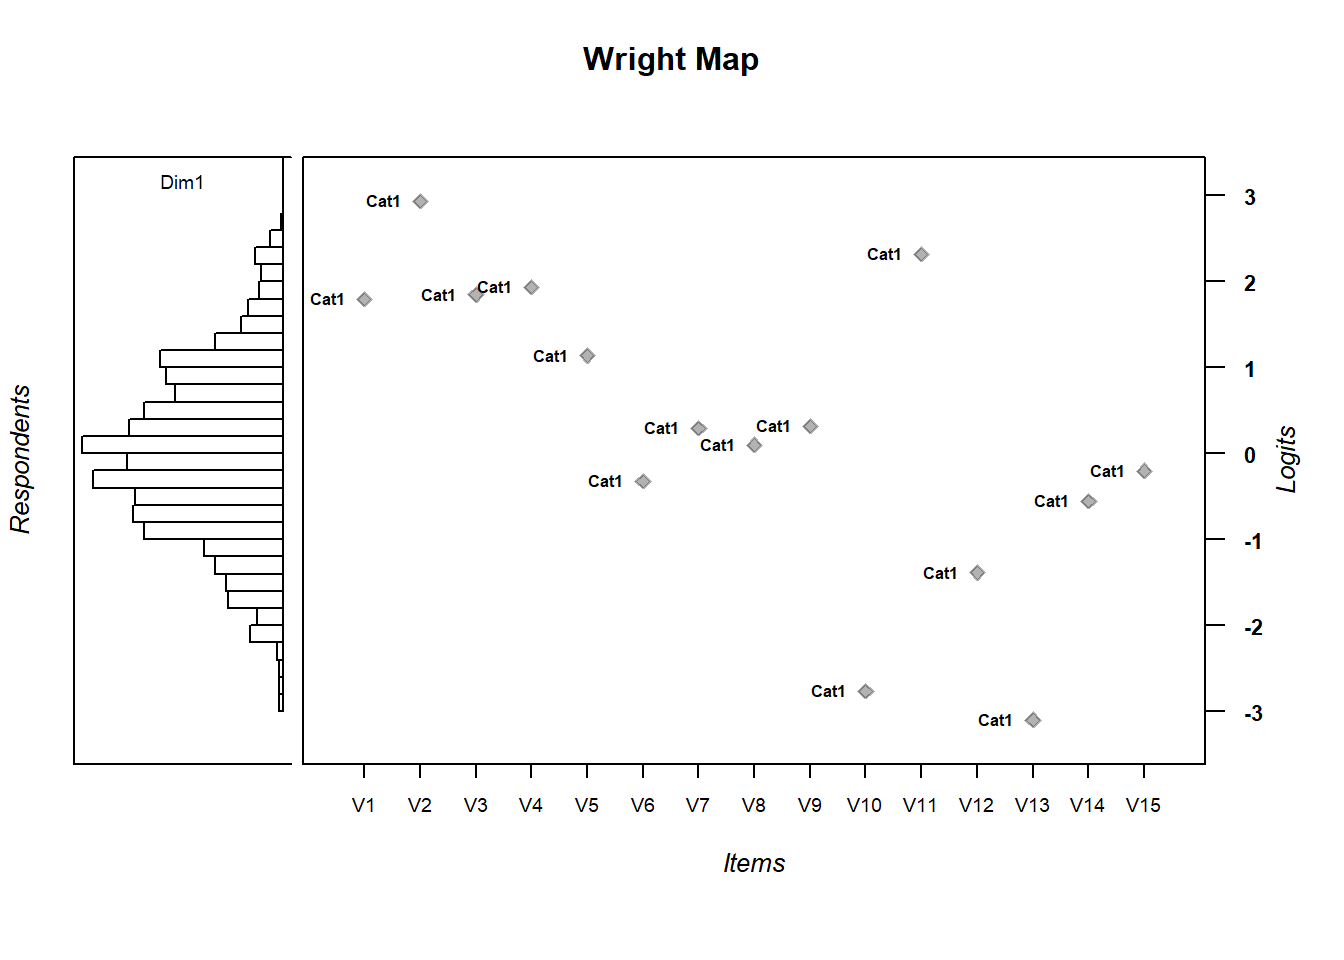
\includegraphics{Rasch_Biome_files/figure-latex/unnamed-chunk-38-1.pdf}

\begin{Shaded}
\begin{Highlighting}[]
\FunctionTok{mean}\NormalTok{(PersonAbility)}
\end{Highlighting}
\end{Shaded}

\begin{verbatim}
## [1] 0.001822466
\end{verbatim}

\begin{Shaded}
\begin{Highlighting}[]
\FunctionTok{sd}\NormalTok{(PersonAbility)}
\end{Highlighting}
\end{Shaded}

\begin{verbatim}
## [1] 1.205116
\end{verbatim}

\hypertarget{wright-map}{%
\section{Wright Map}\label{wright-map}}

To visualize the relationship between item difficulty and person ability distributions, call the WrightMap package installed previously. We'll generate a simple WrightMap. We'll clean it up a little bit by removing some elements

\begin{Shaded}
\begin{Highlighting}[]
\FunctionTok{library}\NormalTok{(WrightMap)}
\FunctionTok{IRT.WrightMap}\NormalTok{(mod1)}
\end{Highlighting}
\end{Shaded}

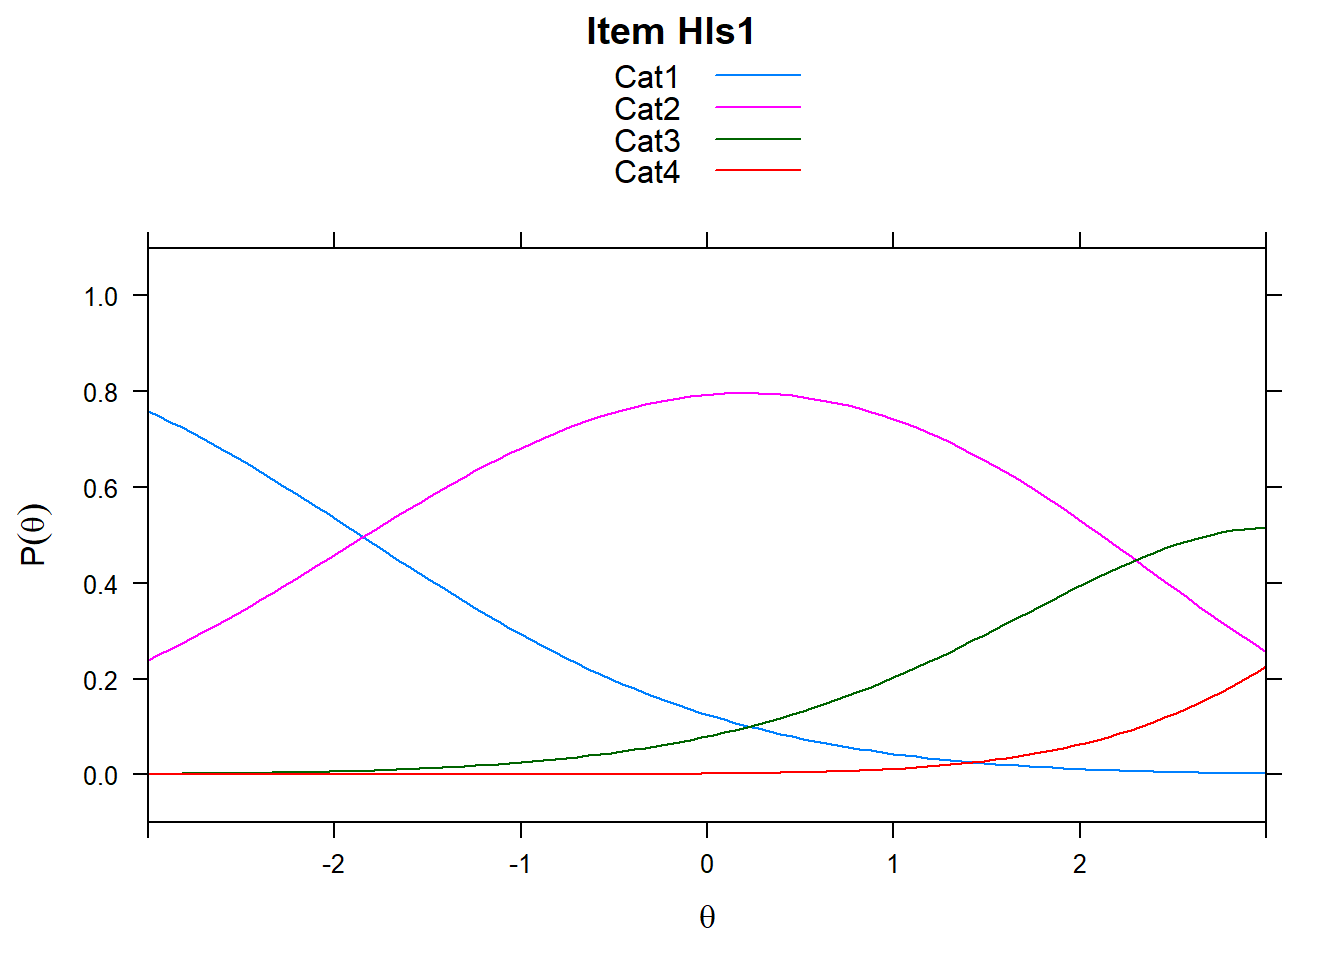
\includegraphics{Rasch_Biome_files/figure-latex/unnamed-chunk-39-1.pdf}

\begin{Shaded}
\begin{Highlighting}[]
\FunctionTok{IRT.WrightMap}\NormalTok{(mod1, }\AttributeTok{show.thr.lab=}\ConstantTok{FALSE}\NormalTok{)}
\end{Highlighting}
\end{Shaded}

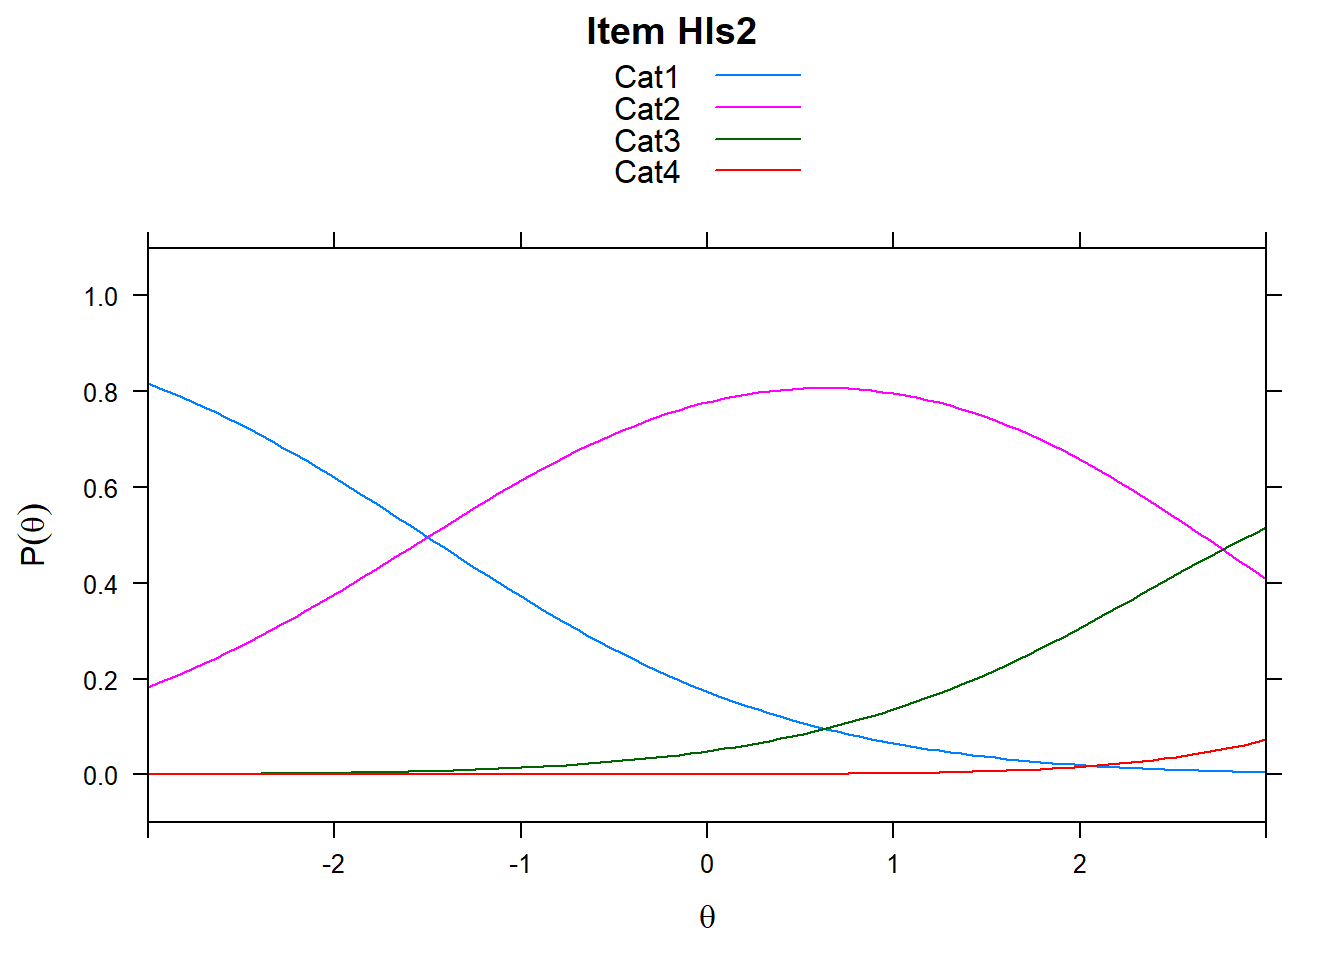
\includegraphics{Rasch_Biome_files/figure-latex/unnamed-chunk-39-2.pdf}

\hypertarget{exercise-2}{%
\subsection{Exercise:}\label{exercise-2}}

\begin{enumerate}
\def\labelenumi{\arabic{enumi}.}
\tightlist
\item
  Are the items appropriately targeted to the ability level of the population?
\item
  Why do you think?
\end{enumerate}

\hypertarget{polytomous-items}{%
\chapter{Polytomous Items}\label{polytomous-items}}

\hypertarget{polytymous-item-types-anything-with-a-rating-scale}{%
\section{Polytymous item types (anything with a rating Scale)}\label{polytymous-item-types-anything-with-a-rating-scale}}

We can use the Rasch Partial Credit Model (PCM) to look at polytomous data too. We'll start by bringing in the polytomous items from the survey. Note that TAM needs the bottom category to be coded as 0, so you may need to recode.

\begin{verbatim}
hls2 <- read.csv("hls_poly_scale.csv")
\end{verbatim}

We see these items are coded with four categories. And the categories are fairly sparse in the 4 fourth category (coded 3, since indexed starting with 0). This may be motivation to collapse categories.

\begin{Shaded}
\begin{Highlighting}[]
\FunctionTok{head}\NormalTok{(hls2)}
\end{Highlighting}
\end{Shaded}

\begin{verbatim}
##   Hls1 Hls2 Hls3 Hls4 Hls5 Hls6 Hls7 Hls8 Hls9 Hls10 Hls11
## 1    1    1    1    0    1    1    0    2    1     1     2
## 2    2    1    1    1    2    1    1    2    1     1     2
## 3    0    1    1    1    1    1    1    2    1     0     1
## 4    1    1    0    0    2    1    0    1    0     0     2
## 5    1    1    0    0    1    0    0    2    0     0     2
## 6    1    1    1    1    2    1    1    1    1     0     2
##   Hls12 Hls13 Hls14 Hls15 Hls16
## 1     1     1     0     1     1
## 2     2     2     1     1     2
## 3     2     1     1     1     1
## 4     1     1     1     2     1
## 5     2     2     1     1     2
## 6     2     2     1     2     1
\end{verbatim}

\begin{Shaded}
\begin{Highlighting}[]
\FunctionTok{apply}\NormalTok{(hls2, }\DecValTok{2}\NormalTok{, table)}
\end{Highlighting}
\end{Shaded}

\begin{verbatim}
##   Hls1 Hls2 Hls3 Hls4 Hls5 Hls6 Hls7 Hls8 Hls9 Hls10 Hls11
## 0   63   76  129  160   65   90  140   50  146   139    47
## 1  204  207  176  148  166  196  162  154  144   163   116
## 2   44   32   11    7   78   26   12  101   21    13   130
## 3    6    2    1    2    8    5    3   12    6     2    24
##   Hls12 Hls13 Hls14 Hls15 Hls16
## 0    44    52    64    52    69
## 1   138   176   181   148   185
## 2   119    83    60   105    57
## 3    16     6    12    12     6
\end{verbatim}

\begin{verbatim}
View(hls2)
\end{verbatim}

TAM will automatically run the PCM when our data is polytomous. There are other model-types for polytomous data such as the rating scale model. This may be more appropriate for Likert-type items. For more information, read TAM documentation or see the reference list (Bond \& Fox, 2007)

\begin{Shaded}
\begin{Highlighting}[]
\NormalTok{mod2 }\OtherTok{\textless{}{-}} \FunctionTok{tam}\NormalTok{(hls2)}
\end{Highlighting}
\end{Shaded}

\begin{Shaded}
\begin{Highlighting}[]
\FunctionTok{summary}\NormalTok{(mod2)}
\end{Highlighting}
\end{Shaded}

\begin{verbatim}
## ------------------------------------------------------------
## TAM 3.5-19 (2020-05-05 22:45:39) 
## R version 3.6.0 (2019-04-26) x86_64, mingw32 | nodename=LAPTOP-K7402PLE | login=katzd 
## 
## Date of Analysis: 2021-02-07 11:13:16 
## Time difference of 0.4680002 secs
## Computation time: 0.4680002 
## 
## Multidimensional Item Response Model in TAM 
## 
## IRT Model: 1PL
## Call:
## tam.mml(resp = resp)
## 
## ------------------------------------------------------------
## Number of iterations = 57 
## Numeric integration with 21 integration points
## 
## Deviance = 8371.25 
## Log likelihood = -4185.63 
## Number of persons = 317 
## Number of persons used = 317 
## Number of items = 16 
## Number of estimated parameters = 49 
##     Item threshold parameters = 48 
##     Item slope parameters = 0 
##     Regression parameters = 0 
##     Variance/covariance parameters = 1 
## 
## AIC = 8469  | penalty=98    | AIC=-2*LL + 2*p 
## AIC3 = 8518  | penalty=147    | AIC3=-2*LL + 3*p 
## BIC = 8653  | penalty=282.19    | BIC=-2*LL + log(n)*p 
## aBIC = 8497  | penalty=126.15    | aBIC=-2*LL + log((n-2)/24)*p  (adjusted BIC) 
## CAIC = 8702  | penalty=331.19    | CAIC=-2*LL + [log(n)+1]*p  (consistent AIC) 
## AICc = 8488  | penalty=116.35    | AICc=-2*LL + 2*p + 2*p*(p+1)/(n-p-1)  (bias corrected AIC) 
## GHP = 0.8349     | GHP=( -LL + p ) / (#Persons * #Items)  (Gilula-Haberman log penalty) 
## 
## ------------------------------------------------------------
## EAP Reliability
## [1] 0.914
## ------------------------------------------------------------
## Covariances and Variances
##       [,1]
## [1,] 2.615
## ------------------------------------------------------------
## Correlations and Standard Deviations (in the diagonal)
##       [,1]
## [1,] 1.617
## ------------------------------------------------------------
## Regression Coefficients
##      [,1]
## [1,]    0
## ------------------------------------------------------------
## Item Parameters -A*Xsi
##     item   N     M xsi.item AXsi_.Cat1 AXsi_.Cat2
## 1   Hls1 317 0.978    1.427     -1.846      0.452
## 2   Hls2 317 0.874    2.074     -1.502      1.263
## 3   Hls3 317 0.634    2.903     -0.381      3.581
## 4   Hls4 317 0.530    2.809      0.176      4.500
## 5   Hls5 317 1.091    1.198     -1.684     -0.302
## 6   Hls6 317 0.830    1.818     -1.155      1.784
## 7   Hls7 317 0.615    2.455     -0.166      3.587
## 8   Hls8 317 1.237    0.781     -2.136     -1.239
## 9   Hls9 317 0.644    2.098     -0.008      2.982
## 10 Hls10 317 0.615    2.630     -0.183      3.511
## 11 Hls11 317 1.413    0.325     -2.106     -1.934
## 12 Hls12 317 1.338    0.512     -2.318     -1.805
## 13 Hls13 317 1.136    1.162     -2.127     -0.789
## 14 Hls14 317 1.063    1.070     -1.762      0.000
## 15 Hls15 317 1.243    0.792     -2.043     -1.232
## 16 Hls16 317 1.000    1.434     -1.629      0.278
##    AXsi_.Cat3 B.Cat1.Dim1 B.Cat2.Dim1 B.Cat3.Dim1
## 1       4.282           1           2           3
## 2       6.221           1           2           3
## 3       8.709           1           2           3
## 4       8.428           1           2           3
## 5       3.595           1           2           3
## 6       5.455           1           2           3
## 7       7.364           1           2           3
## 8       2.342           1           2           3
## 9       6.295           1           2           3
## 10      7.890           1           2           3
## 11      0.974           1           2           3
## 12      1.537           1           2           3
## 13      3.487           1           2           3
## 14      3.209           1           2           3
## 15      2.376           1           2           3
## 16      4.303           1           2           3
## 
## Item Parameters Xsi
##               xsi se.xsi
## Hls1_Cat1  -1.846  0.177
## Hls1_Cat2   2.298  0.174
## Hls1_Cat3   3.830  0.464
## Hls2_Cat1  -1.502  0.164
## Hls2_Cat2   2.765  0.200
## Hls2_Cat3   4.958  0.780
## Hls3_Cat1  -0.381  0.138
## Hls3_Cat2   3.962  0.321
## Hls3_Cat3   5.127  1.117
## Hls4_Cat1   0.176  0.133
## Hls4_Cat2   4.325  0.378
## Hls4_Cat3   3.927  0.853
## Hls5_Cat1  -1.684  0.178
## Hls5_Cat2   1.382  0.147
## Hls5_Cat3   3.897  0.394
## Hls6_Cat1  -1.155  0.154
## Hls6_Cat2   2.939  0.211
## Hls6_Cat3   3.671  0.519
## Hls7_Cat1  -0.166  0.136
## Hls7_Cat2   3.753  0.295
## Hls7_Cat3   3.776  0.689
## Hls8_Cat1  -2.136  0.199
## Hls8_Cat2   0.897  0.139
## Hls8_Cat3   3.581  0.324
## Hls9_Cat1  -0.008  0.136
## Hls9_Cat2   2.990  0.229
## Hls9_Cat3   3.313  0.482
## Hls10_Cat1 -0.183  0.136
## Hls10_Cat2  3.695  0.292
## Hls10_Cat3  4.379  0.822
## Hls11_Cat1 -2.106  0.210
## Hls11_Cat2  0.173  0.138
## Hls11_Cat3  2.907  0.235
## Hls12_Cat1 -2.318  0.212
## Hls12_Cat2  0.513  0.136
## Hls12_Cat3  3.342  0.282
## Hls13_Cat1 -2.127  0.194
## Hls13_Cat2  1.339  0.144
## Hls13_Cat3  4.276  0.449
## Hls14_Cat1 -1.761  0.178
## Hls14_Cat2  1.762  0.155
## Hls14_Cat3  3.208  0.331
## Hls15_Cat1 -2.042  0.197
## Hls15_Cat2  0.810  0.138
## Hls15_Cat3  3.609  0.323
## Hls16_Cat1 -1.629  0.172
## Hls16_Cat2  1.907  0.160
## Hls16_Cat3  4.025  0.457
## 
## Item Parameters in IRT parameterization
##     item alpha  beta tau.Cat1 tau.Cat2 tau.Cat3
## 1   Hls1     1 1.427   -3.274    0.871    2.403
## 2   Hls2     1 2.074   -3.575    0.691    2.885
## 3   Hls3     1 2.903   -3.284    1.059    2.224
## 4   Hls4     1 2.809   -2.633    1.515    1.118
## 5   Hls5     1 1.198   -2.883    0.184    2.699
## 6   Hls6     1 1.818   -2.974    1.121    1.853
## 7   Hls7     1 2.455   -2.620    1.299    1.322
## 8   Hls8     1 0.781   -2.917    0.116    2.800
## 9   Hls9     1 2.098   -2.106    0.891    1.215
## 10 Hls10     1 2.630   -2.814    1.065    1.749
## 11 Hls11     1 0.325   -2.431   -0.152    2.583
## 12 Hls12     1 0.512   -2.830    0.001    2.830
## 13 Hls13     1 1.162   -3.290    0.176    3.113
## 14 Hls14     1 1.070   -2.831    0.692    2.139
## 15 Hls15     1 0.792   -2.835    0.018    2.816
## 16 Hls16     1 1.434   -3.063    0.472    2.590
\end{verbatim}

\hypertarget{item-difficulties-1}{%
\section{Item Difficulties}\label{item-difficulties-1}}

Now we'll get item and person characteristics just like before.

TAM also uses the delta-tau paramaterization of the partial credit model as default. The problem is, we may be curious about the thresholds (cumulative), the overall item difficulty, and steps. TAM provides this all but it's not straightforward.

\begin{Shaded}
\begin{Highlighting}[]
\CommentTok{\# Deltas}


\NormalTok{xsi }\OtherTok{\textless{}{-}}\NormalTok{ mod2}\SpecialCharTok{$}\NormalTok{xsi}

\CommentTok{\# get thresholds {-} Thurstone Thresholds get the cumulative values}
\NormalTok{tthresh }\OtherTok{\textless{}{-}} \FunctionTok{tam.threshold}\NormalTok{(mod2)}

\CommentTok{\# Delta{-}tau parameters}
\NormalTok{delta\_tau }\OtherTok{\textless{}{-}}\NormalTok{ mod2}\SpecialCharTok{$}\NormalTok{item\_irt}

\CommentTok{\# we have to do some addition...}


\NormalTok{xsi}
\end{Highlighting}
\end{Shaded}

\begin{verbatim}
##                     xsi    se.xsi
## Hls1_Cat1  -1.846046710 0.1770841
## Hls1_Cat2   2.298334842 0.1736858
## Hls1_Cat3   3.830385868 0.4635448
## Hls2_Cat1  -1.501715752 0.1640914
## Hls2_Cat2   2.764560868 0.2004621
## Hls2_Cat3   4.958324889 0.7804292
## Hls3_Cat1  -0.380834628 0.1378983
## Hls3_Cat2   3.962213547 0.3205437
## Hls3_Cat3   5.127428610 1.1165768
## Hls4_Cat1   0.175976124 0.1331498
## Hls4_Cat2   4.324558567 0.3775359
## Hls4_Cat3   3.927492901 0.8526291
## Hls5_Cat1  -1.684131262 0.1781274
## Hls5_Cat2   1.381933373 0.1467223
## Hls5_Cat3   3.897482578 0.3943440
## Hls6_Cat1  -1.155351142 0.1543659
## Hls6_Cat2   2.939344680 0.2113184
## Hls6_Cat3   3.671463609 0.5189345
## Hls7_Cat1  -0.165823435 0.1358793
## Hls7_Cat2   3.753328170 0.2949727
## Hls7_Cat3   3.776319530 0.6885511
## Hls8_Cat1  -2.135935885 0.1992731
## Hls8_Cat2   0.896643565 0.1385362
## Hls8_Cat3   3.581083599 0.3235907
## Hls9_Cat1  -0.008019089 0.1360316
## Hls9_Cat2   2.989853095 0.2288433
## Hls9_Cat3   3.313295753 0.4819018
## Hls10_Cat1 -0.183297684 0.1360561
## Hls10_Cat2  3.694746057 0.2921816
## Hls10_Cat3  4.379242422 0.8215605
## Hls11_Cat1 -2.106058995 0.2097751
## Hls11_Cat2  0.172650186 0.1377271
## Hls11_Cat3  2.907183948 0.2353937
## Hls12_Cat1 -2.317865929 0.2117123
## Hls12_Cat2  0.513325662 0.1362435
## Hls12_Cat3  3.342199604 0.2821645
## Hls13_Cat1 -2.127336182 0.1938394
## Hls13_Cat2  1.338677184 0.1444056
## Hls13_Cat3  4.275574749 0.4493420
## Hls14_Cat1 -1.761463128 0.1777770
## Hls14_Cat2  1.762102813 0.1550751
## Hls14_Cat3  3.208316423 0.3314447
## Hls15_Cat1 -2.042459839 0.1969236
## Hls15_Cat2  0.810466042 0.1380178
## Hls15_Cat3  3.608588261 0.3230206
## Hls16_Cat1 -1.628691156 0.1721913
## Hls16_Cat2  1.906727817 0.1604086
## Hls16_Cat3  4.024764112 0.4574405
\end{verbatim}

\begin{Shaded}
\begin{Highlighting}[]
\NormalTok{delta\_tau}
\end{Highlighting}
\end{Shaded}

\begin{verbatim}
##     item alpha      beta  tau.Cat1      tau.Cat2 tau.Cat3
## 1   Hls1     1 1.4274710 -3.273603  0.8707754118 2.402828
## 2   Hls2     1 2.0736329 -3.575436  0.6908361981 2.884600
## 3   Hls3     1 2.9028463 -3.283771  1.0592759982 2.224495
## 4   Hls4     1 2.8092628 -2.633376  1.5152150567 1.118161
## 5   Hls5     1 1.1983411 -2.882556  0.1835035073 2.699053
## 6   Hls6     1 1.8184015 -2.973840  1.1208578911 1.852982
## 7   Hls7     1 2.4545273 -2.620439  1.2987189037 1.321721
## 8   Hls8     1 0.7805103 -2.916528  0.1160446178 2.800483
## 9   Hls9     1 2.0983006 -2.106406  0.8914751897 1.214930
## 10 Hls10     1 2.6301446 -2.813531  1.0645139316 1.749018
## 11 Hls11     1 0.3245074 -2.430645 -0.1519433803 2.582588
## 12 Hls12     1 0.5124669 -2.830413  0.0007705277 2.829642
## 13 Hls13     1 1.1622166 -3.289636  0.1763701702 3.113266
## 14 Hls14     1 1.0695679 -2.831114  0.6924494287 2.138665
## 15 Hls15     1 0.7921115 -2.834653  0.0182660931 2.816387
## 16 Hls16     1 1.4341793 -3.062956  0.4724593127 2.590496
\end{verbatim}

\begin{Shaded}
\begin{Highlighting}[]
\NormalTok{mod2}\SpecialCharTok{$}\NormalTok{item }\CommentTok{\#PCM2 type parameteris}
\end{Highlighting}
\end{Shaded}

\begin{verbatim}
##        item   N         M  xsi.item   AXsi_.Cat1
## Hls1   Hls1 317 0.9779180 1.4274710 -1.846131898
## Hls2   Hls2 317 0.8738170 2.0736329 -1.501802830
## Hls3   Hls3 317 0.6340694 2.9028463 -0.380924234
## Hls4   Hls4 317 0.5299685 2.8092628  0.175886380
## Hls5   Hls5 317 1.0914826 1.1983411 -1.684215070
## Hls6   Hls6 317 0.8296530 1.8184015 -1.155438051
## Hls7   Hls7 317 0.6151420 2.4545273 -0.165912194
## Hls8   Hls8 317 1.2365931 0.7805103 -2.136017661
## Hls9   Hls9 317 0.6435331 2.0983006 -0.008105079
## Hls10 Hls10 317 0.6151420 2.6301446 -0.183386855
## Hls11 Hls11 317 1.4132492 0.3245074 -2.106137069
## Hls12 Hls12 317 1.3375394 0.5124669 -2.317946089
## Hls13 Hls13 317 1.1356467 1.1622166 -2.127419718
## Hls14 Hls14 317 1.0630915 1.0695679 -1.761546575
## Hls15 Hls15 317 1.2429022 0.7921115 -2.042541519
## Hls16 Hls16 317 1.0000000 1.4341793 -1.628776280
##          AXsi_.Cat2 AXsi_.Cat3 B.Cat1.Dim1 B.Cat2.Dim1
## Hls1   0.4521145624  4.2824131           1           2
## Hls2   1.2626663181  6.2208988           1           2
## Hls3   3.5811980586  8.7085389           1           2
## Hls4   4.5003642315  8.4277884           1           2
## Hls5  -0.3023704998  3.5950232           1           2
## Hls6   1.7838213033  5.4552044           1           2
## Hls7   3.5873340076  7.3635819           1           2
## Hls8  -1.2394627171  2.3415310           1           2
## Hls9   2.9816706902  6.2949017           1           2
## Hls10  3.5112716780  7.8904338           1           2
## Hls11 -1.9335729998  0.9735223           1           2
## Hls12 -1.8047086322  1.5374008           1           2
## Hls13 -0.7888329123  3.4866499           1           2
## Hls14  0.0004707108  3.2087036           1           2
## Hls15 -1.2321639435  2.3763344           1           2
## Hls16  0.2778623406  4.3025379           1           2
##       B.Cat3.Dim1
## Hls1            3
## Hls2            3
## Hls3            3
## Hls4            3
## Hls5            3
## Hls6            3
## Hls7            3
## Hls8            3
## Hls9            3
## Hls10           3
## Hls11           3
## Hls12           3
## Hls13           3
## Hls14           3
## Hls15           3
## Hls16           3
\end{verbatim}

\begin{Shaded}
\begin{Highlighting}[]
\CommentTok{\#note, if you want to see this in your viewer, you can also use View().}
\end{Highlighting}
\end{Shaded}

Going between the different parameterizations:
First, look at \texttt{xsi} Hls1 categories. As a reminder, the item has 4 categories, thus three thresholds. We see, that: -1.8460467, 2.2983348, 3.8303859 gives us deltas/steps for the first the three steps of \texttt{Hls1}.

Now, look at 1, 1, 1.42747104894573, -3.27360294723895, 0.870775411784539, 2.40282753545441. Believe it or not, this gives us the same information. How, so?

\begin{Shaded}
\begin{Highlighting}[]
\NormalTok{delta\_tau }\OtherTok{\textless{}{-}}\NormalTok{ delta\_tau }\SpecialCharTok{\%\textgreater{}\%}
  \FunctionTok{mutate}\NormalTok{(}\AttributeTok{HLS\_cat1 =}\NormalTok{ beta }\SpecialCharTok{+}\NormalTok{ tau.Cat1,}
         \AttributeTok{HLS\_cat2 =}\NormalTok{ beta }\SpecialCharTok{+}\NormalTok{ tau.Cat2,}
         \AttributeTok{HLS\_cat3 =}\NormalTok{ beta }\SpecialCharTok{+}\NormalTok{ tau.Cat3)}

\NormalTok{delta\_tau}
\end{Highlighting}
\end{Shaded}

\begin{verbatim}
##     item alpha      beta  tau.Cat1      tau.Cat2 tau.Cat3
## 1   Hls1     1 1.4274710 -3.273603  0.8707754118 2.402828
## 2   Hls2     1 2.0736329 -3.575436  0.6908361981 2.884600
## 3   Hls3     1 2.9028463 -3.283771  1.0592759982 2.224495
## 4   Hls4     1 2.8092628 -2.633376  1.5152150567 1.118161
## 5   Hls5     1 1.1983411 -2.882556  0.1835035073 2.699053
## 6   Hls6     1 1.8184015 -2.973840  1.1208578911 1.852982
## 7   Hls7     1 2.4545273 -2.620439  1.2987189037 1.321721
## 8   Hls8     1 0.7805103 -2.916528  0.1160446178 2.800483
## 9   Hls9     1 2.0983006 -2.106406  0.8914751897 1.214930
## 10 Hls10     1 2.6301446 -2.813531  1.0645139316 1.749018
## 11 Hls11     1 0.3245074 -2.430645 -0.1519433803 2.582588
## 12 Hls12     1 0.5124669 -2.830413  0.0007705277 2.829642
## 13 Hls13     1 1.1622166 -3.289636  0.1763701702 3.113266
## 14 Hls14     1 1.0695679 -2.831114  0.6924494287 2.138665
## 15 Hls15     1 0.7921115 -2.834653  0.0182660931 2.816387
## 16 Hls16     1 1.4341793 -3.062956  0.4724593127 2.590496
##        HLS_cat1  HLS_cat2 HLS_cat3
## 1  -1.846131898 2.2982465 3.830299
## 2  -1.501802830 2.7644691 4.958233
## 3  -0.380924234 3.9621223 5.127341
## 4   0.175886380 4.3244779 3.927424
## 5  -1.684215070 1.3818446 3.897394
## 6  -1.155438051 2.9392594 3.671383
## 7  -0.165912194 3.7532462 3.776248
## 8  -2.136017661 0.8965549 3.580994
## 9  -0.008105079 2.9897758 3.313231
## 10 -0.183386855 3.6946585 4.379162
## 11 -2.106137069 0.1725641 2.907095
## 12 -2.317946089 0.5132375 3.342109
## 13 -2.127419718 1.3385868 4.275483
## 14 -1.761546575 1.7620173 3.208233
## 15 -2.042541519 0.8103776 3.608498
## 16 -1.628776280 1.9066386 4.024676
\end{verbatim}

Note, now, that, that the delta\_tau ``item difficulty'' (or \texttt{beta}) + \texttt{tau} gets you back to the estimates of \texttt{xsi}

This is the difference between two different parameterization in the PCM model. One parametrization is:
\[P(X_{si} = x) = \frac{exp[\sum_{k=0}^x(\theta_s-\delta_{ik})]}{\sum_{h=0}^{m_i}exp[\sum_{k=0}^h(\theta_s-\delta_{ik})]}\].

This is roughly what you're seeing for the \texttt{xsi} estimates. Here, \texttt{k} indexes item category, \(\delta\) is the item, \texttt{s} indexes student.

The other parameterization, delta\_tau, helps us nicely transition to the Rating Scale model, showing that the Rating Scale Model is a special case of the PCM.

\[P(X_{si} = x) = \frac{exp[\sum_{k=0}^x(\theta_s-\delta_{i}+\tau_{ik})]}{\sum_{h=0}^{m_i}exp[\sum_{k=0}^h(\theta_s-\delta_{i} + \tau_{ik})]}\].

Here, \(\delta_i\) is the item, and \(\tau\) is the item category. In the PCM, the \tau is item specific, it's the ``jump'' of the category from the overall item difficulty.

In the rating scale model, the delta\_tau parameterization is used, but each \tau is the same, or, at leas, each deviance amount is the same.

The parameterization in \texttt{mod2} item lets you go between different parameterizations if you so choose. For instance, \texttt{mod2\$item} gives you an \texttt{xsi.item} column that is the item difficulty in the \texttt{PCM2} parameterizations. The \texttt{AXsi\_.Cat\#} items are the sums of the \texttt{xsi} delta/step parameters up to that step.

\hypertarget{person-ability-theta-estimates}{%
\section{Person ability (theta) estimates}\label{person-ability-theta-estimates}}

\begin{Shaded}
\begin{Highlighting}[]
\NormalTok{WLE.ability.poly }\OtherTok{\textless{}{-}} \FunctionTok{tam.wle}\NormalTok{(mod2)}
\end{Highlighting}
\end{Shaded}

\begin{verbatim}
## Iteration in WLE/MLE estimation  1   | Maximal change  2.6967 
## Iteration in WLE/MLE estimation  2   | Maximal change  2.1777 
## Iteration in WLE/MLE estimation  3   | Maximal change  0.368 
## Iteration in WLE/MLE estimation  4   | Maximal change  0.0135 
## Iteration in WLE/MLE estimation  5   | Maximal change  3e-04 
## Iteration in WLE/MLE estimation  6   | Maximal change  0 
## ----
##  WLE Reliability= 0.9
\end{verbatim}

\begin{Shaded}
\begin{Highlighting}[]
\NormalTok{person.ability.poly }\OtherTok{\textless{}{-}}\NormalTok{ WLE.ability.poly}\SpecialCharTok{$}\NormalTok{theta}
\FunctionTok{head}\NormalTok{(person.ability.poly)}
\end{Highlighting}
\end{Shaded}

\begin{verbatim}
## [1]  0.07670224  1.74460893  0.29326740 -0.14106713
## [5]  0.07670224  1.14369491
\end{verbatim}

\hypertarget{item-fit-statistics}{%
\section{Item fit statistics}\label{item-fit-statistics}}

The rest of the workflow from here now is pretty similar with a few different challenges

We need to get infit and outfit (mean square) for each item. Only now it'll be by item category.

\begin{Shaded}
\begin{Highlighting}[]
\NormalTok{Fit.poly }\OtherTok{\textless{}{-}} \FunctionTok{tam.fit}\NormalTok{(mod2)}
\end{Highlighting}
\end{Shaded}

\begin{verbatim}
## Item fit calculation based on 100 simulations
## |**********|
## |----------|
\end{verbatim}

\begin{verbatim}
Fit.poly$itemfit
\end{verbatim}

\begin{Shaded}
\begin{Highlighting}[]
\FunctionTok{kable}\NormalTok{(Fit.poly}\SpecialCharTok{$}\NormalTok{itemfit)}
\end{Highlighting}
\end{Shaded}

\begin{tabular}{l|r|r|r|r|r|r|r|r}
\hline
parameter & Outfit & Outfit\_t & Outfit\_p & Outfit\_pholm & Infit & Infit\_t & Infit\_p & Infit\_pholm\\
\hline
Hls1\_Cat1 & 3.1786296 & 11.8472306 & 0.0000000 & 0.0000000 & 1.0328356 & 0.3284381 & 0.7425805 & 1\\
\hline
Hls1\_Cat2 & 4.7788366 & 15.8596192 & 0.0000000 & 0.0000000 & 1.1199215 & 1.1629930 & 0.2448323 & 1\\
\hline
Hls1\_Cat3 & 7163.1677884 & 93.2193005 & 0.0000000 & 0.0000000 & 0.9591327 & 0.0083343 & 0.9933503 & 1\\
\hline
Hls2\_Cat1 & 20.6541992 & 47.2797827 & 0.0000000 & 0.0000000 & 1.0744346 & 0.7727689 & 0.4396591 & 1\\
\hline
Hls2\_Cat2 & 0.9152582 & -0.6672976 & 0.5045820 & 1.0000000 & 1.0403417 & 0.3371105 & 0.7360336 & 1\\
\hline
Hls2\_Cat3 & 0.8174772 & -0.2723914 & 0.7853210 & 1.0000000 & 1.4075029 & 0.7797023 & 0.4355661 & 1\\
\hline
Hls3\_Cat1 & 0.9296682 & -1.1199941 & 0.2627163 & 1.0000000 & 0.9594710 & -0.6265610 & 0.5309470 & 1\\
\hline
Hls3\_Cat2 & 0.8931944 & -0.4272622 & 0.6691884 & 1.0000000 & 0.9127064 & -0.2647029 & 0.7912383 & 1\\
\hline
Hls3\_Cat3 & 0.0145564 & -2.4699143 & 0.0135145 & 0.3648926 & 0.8602399 & 0.0549309 & 0.9561935 & 1\\
\hline
Hls4\_Cat1 & 0.8674859 & -2.5424932 & 0.0110065 & 0.3081813 & 0.9301286 & -1.2999636 & 0.1936135 & 1\\
\hline
Hls4\_Cat2 & 0.6425444 & -1.3268945 & 0.1845436 & 1.0000000 & 0.8885934 & -0.2733489 & 0.7845850 & 1\\
\hline
Hls4\_Cat3 & 0.0102458 & -3.4460191 & 0.0005689 & 0.0193429 & 0.4041259 & -1.0440147 & 0.2964786 & 1\\
\hline
Hls5\_Cat1 & 0.8053151 & -2.0230329 & 0.0430698 & 0.9475346 & 0.8379377 & -1.5542462 & 0.1201257 & 1\\
\hline
Hls5\_Cat2 & 1.8636547 & 7.1476836 & 0.0000000 & 0.0000000 & 1.0797123 & 1.1698947 & 0.2420434 & 1\\
\hline
Hls5\_Cat3 & 1.9165284 & 1.9415955 & 0.0521861 & 1.0000000 & 1.0768953 & 0.3340262 & 0.7383598 & 1\\
\hline
Hls6\_Cat1 & 0.9189453 & -0.9826259 & 0.3257916 & 1.0000000 & 0.8694677 & -1.5627347 & 0.1181150 & 1\\
\hline
Hls6\_Cat2 & 1.3522319 & 2.0904110 & 0.0365809 & 0.8779414 & 1.0173114 & 0.1616013 & 0.8716199 & 1\\
\hline
Hls6\_Cat3 & 2.9162117 & 2.7657330 & 0.0056795 & 0.1760645 & 1.3107973 & 0.8089227 & 0.4185596 & 1\\
\hline
Hls7\_Cat1 & 0.8337633 & -2.9363469 & 0.0033210 & 0.1095939 & 0.9100411 & -1.5325230 & 0.1253934 & 1\\
\hline
Hls7\_Cat2 & 0.5304334 & -2.4668933 & 0.0136291 & 0.3648926 & 0.9001150 & -0.3805080 & 0.7035684 & 1\\
\hline
Hls7\_Cat3 & 0.8305281 & -0.6847062 & 0.4935294 & 1.0000000 & 1.1754512 & 0.4693030 & 0.6388531 & 1\\
\hline
Hls8\_Cat1 & 0.6232617 & -3.5058867 & 0.0004551 & 0.0159281 & 0.8481463 & -1.2452896 & 0.2130253 & 1\\
\hline
Hls8\_Cat2 & 2.3091650 & 14.1802906 & 0.0000000 & 0.0000000 & 1.0746988 & 1.2866596 & 0.1982130 & 1\\
\hline
Hls8\_Cat3 & 1.3670417 & 1.0429875 & 0.2969541 & 1.0000000 & 0.9520319 & -0.1142403 & 0.9090473 & 1\\
\hline
Hls9\_Cat1 & 0.8818177 & -2.0903473 & 0.0365866 & 0.8779414 & 0.9507722 & -0.8371149 & 0.4025280 & 1\\
\hline
Hls9\_Cat2 & 1.4114300 & 2.1974018 & 0.0279918 & 0.6997941 & 1.0815131 & 0.5490325 & 0.5829831 & 1\\
\hline
Hls9\_Cat3 & 0.8003895 & -0.7182009 & 0.4726334 & 1.0000000 & 0.9428510 & -0.0374113 & 0.9701570 & 1\\
\hline
Hls10\_Cat1 & 1.0210965 & 0.3377758 & 0.7355321 & 1.0000000 & 1.0148962 & 0.2571824 & 0.7970380 & 1\\
\hline
Hls10\_Cat2 & 98.6065575 & 39.3645496 & 0.0000000 & 0.0000000 & 1.1418194 & 0.6616649 & 0.5081860 & 1\\
\hline
Hls10\_Cat3 & 0.5885241 & -0.8680905 & 0.3853448 & 1.0000000 & 1.0131734 & 0.2155321 & 0.8293525 & 1\\
\hline
Hls11\_Cat1 & 0.8114686 & -1.7277106 & 0.0840401 & 1.0000000 & 0.8577507 & -1.1107156 & 0.2666908 & 1\\
\hline
Hls11\_Cat2 & 0.9244416 & -1.3478507 & 0.1777064 & 1.0000000 & 1.0224056 & 0.3947324 & 0.6930404 & 1\\
\hline
Hls11\_Cat3 & 2.0173329 & 4.2908510 & 0.0000178 & 0.0006586 & 0.9967470 & 0.0302450 & 0.9758716 & 1\\
\hline
Hls12\_Cat1 & 0.6844793 & -2.8448343 & 0.0044435 & 0.1421905 & 0.7294653 & -2.2114467 & 0.0270049 & 1\\
\hline
Hls12\_Cat2 & 1.1164697 & 1.7167902 & 0.0860175 & 1.0000000 & 0.9946495 & -0.0878893 & 0.9299646 & 1\\
\hline
Hls12\_Cat3 & 3.0960292 & 5.8262943 & 0.0000000 & 0.0000002 & 1.0365105 & 0.2348176 & 0.8143503 & 1\\
\hline
Hls13\_Cat1 & 0.9486458 & -0.5801593 & 0.5618072 & 1.0000000 & 0.7709388 & -2.0060662 & 0.0448492 & 1\\
\hline
Hls13\_Cat2 & 1.0150495 & 0.2222191 & 0.8241434 & 1.0000000 & 1.0549126 & 0.8445516 & 0.3983613 & 1\\
\hline
Hls13\_Cat3 & 2.1105963 & 1.9774008 & 0.0479963 & 1.0000000 & 0.8989601 & -0.1621237 & 0.8712085 & 1\\
\hline
Hls14\_Cat1 & 0.8218765 & -1.7545179 & 0.0793418 & 1.0000000 & 0.9133679 & -0.7906545 & 0.4291456 & 1\\
\hline
Hls14\_Cat2 & 2.4775838 & 12.0341103 & 0.0000000 & 0.0000000 & 1.0718813 & 0.9185494 & 0.3583313 & 1\\
\hline
Hls14\_Cat3 & 0.6061866 & -1.9385604 & 0.0525549 & 1.0000000 & 0.9793765 & -0.0109348 & 0.9912755 & 1\\
\hline
Hls15\_Cat1 & 0.7123961 & -2.6843279 & 0.0072676 & 0.2180274 & 0.8055118 & -1.6614215 & 0.0966288 & 1\\
\hline
Hls15\_Cat2 & 1.1032820 & 1.7502926 & 0.0800678 & 1.0000000 & 1.0750763 & 1.3107750 & 0.1899338 & 1\\
\hline
Hls15\_Cat3 & 4.4281070 & 6.5959252 & 0.0000000 & 0.0000000 & 0.9589296 & -0.0857018 & 0.9317035 & 1\\
\hline
Hls16\_Cat1 & 1.5180821 & 4.1780228 & 0.0000294 & 0.0010586 & 0.9501315 & -0.4588437 & 0.6463464 & 1\\
\hline
Hls16\_Cat2 & 2.0474712 & 8.9254651 & 0.0000000 & 0.0000000 & 1.0609289 & 0.7244284 & 0.4688028 & 1\\
\hline
Hls16\_Cat3 & 0.3110743 & -2.5708344 & 0.0101454 & 0.2942161 & 0.8198852 & -0.3996161 & 0.6894393 & 1\\
\hline
\end{tabular}

\hypertarget{item-characteristic-curves-but-now-as-thresholds.}{%
\section{Item characteristic curves (but now as thresholds).}\label{item-characteristic-curves-but-now-as-thresholds.}}

There are item characteristic curves (ICCs) for each item choice

\begin{Shaded}
\begin{Highlighting}[]
\NormalTok{tthresh.poly }\OtherTok{\textless{}{-}} \FunctionTok{tam.threshold}\NormalTok{(mod2)}
\FunctionTok{plot}\NormalTok{(mod2, }\AttributeTok{type =} \StringTok{"items"}\NormalTok{)}
\end{Highlighting}
\end{Shaded}

\begin{verbatim}
## Iteration in WLE/MLE estimation  1   | Maximal change  2.6967 
## Iteration in WLE/MLE estimation  2   | Maximal change  2.1777 
## Iteration in WLE/MLE estimation  3   | Maximal change  0.368 
## Iteration in WLE/MLE estimation  4   | Maximal change  0.0135 
## Iteration in WLE/MLE estimation  5   | Maximal change  3e-04 
## Iteration in WLE/MLE estimation  6   | Maximal change  0 
## ----
##  WLE Reliability= 0.9
\end{verbatim}

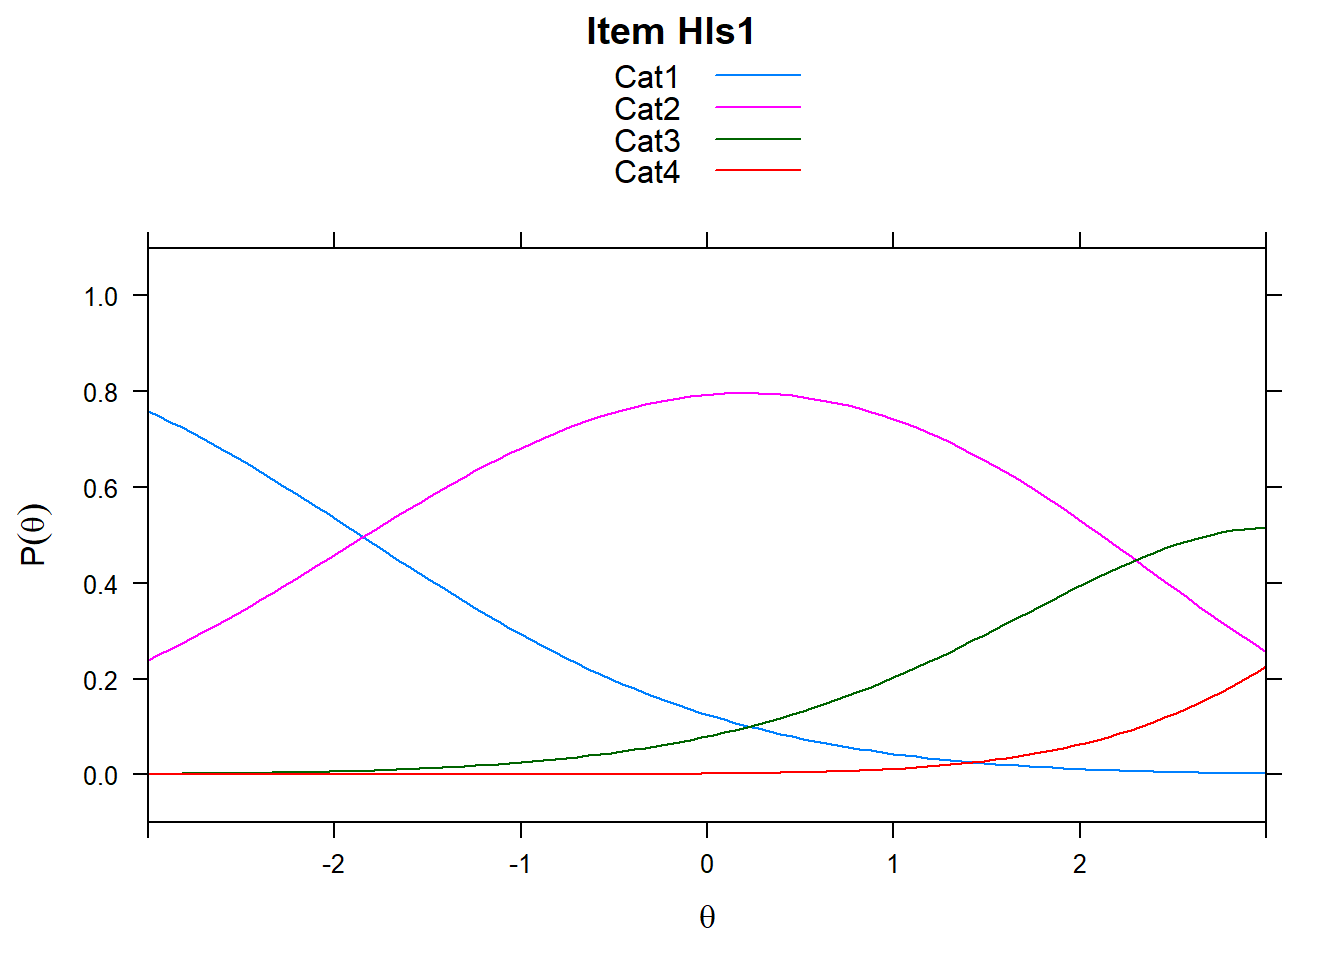
\includegraphics{Rasch_Biome_files/figure-latex/unnamed-chunk-51-1.pdf} 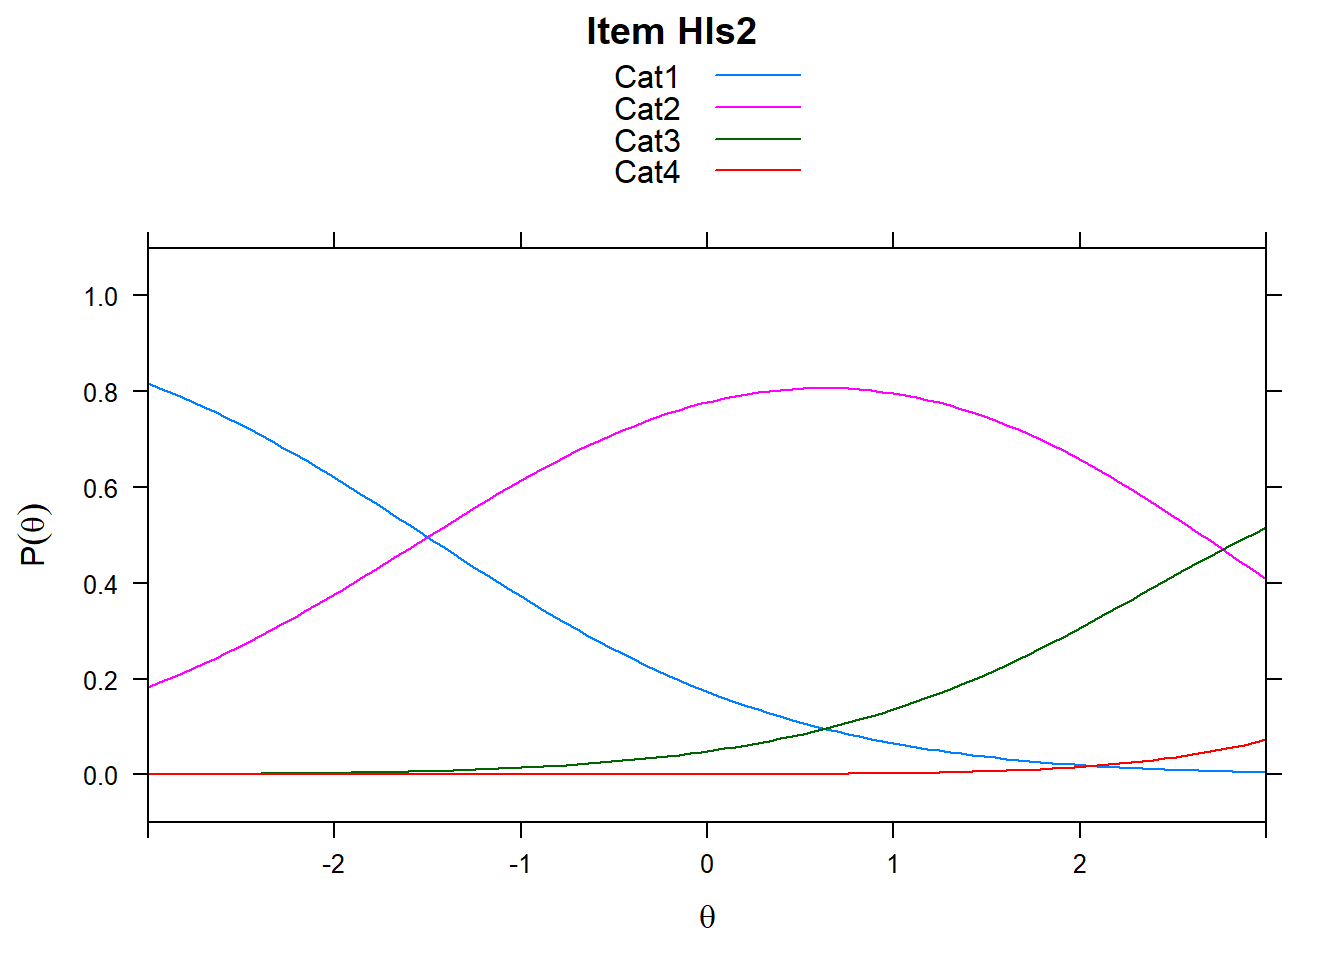
\includegraphics{Rasch_Biome_files/figure-latex/unnamed-chunk-51-2.pdf} 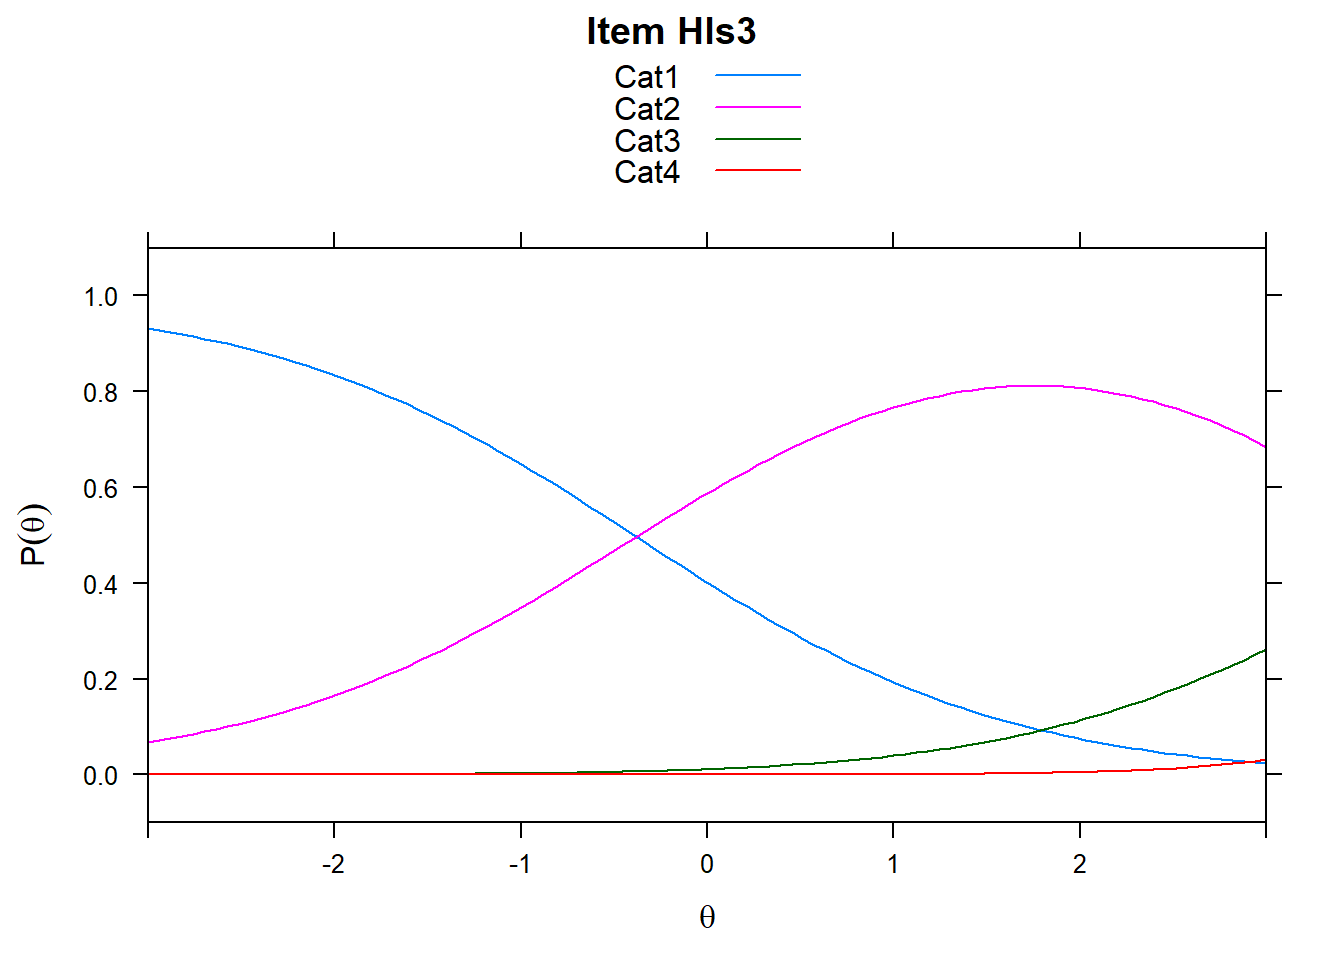
\includegraphics{Rasch_Biome_files/figure-latex/unnamed-chunk-51-3.pdf} 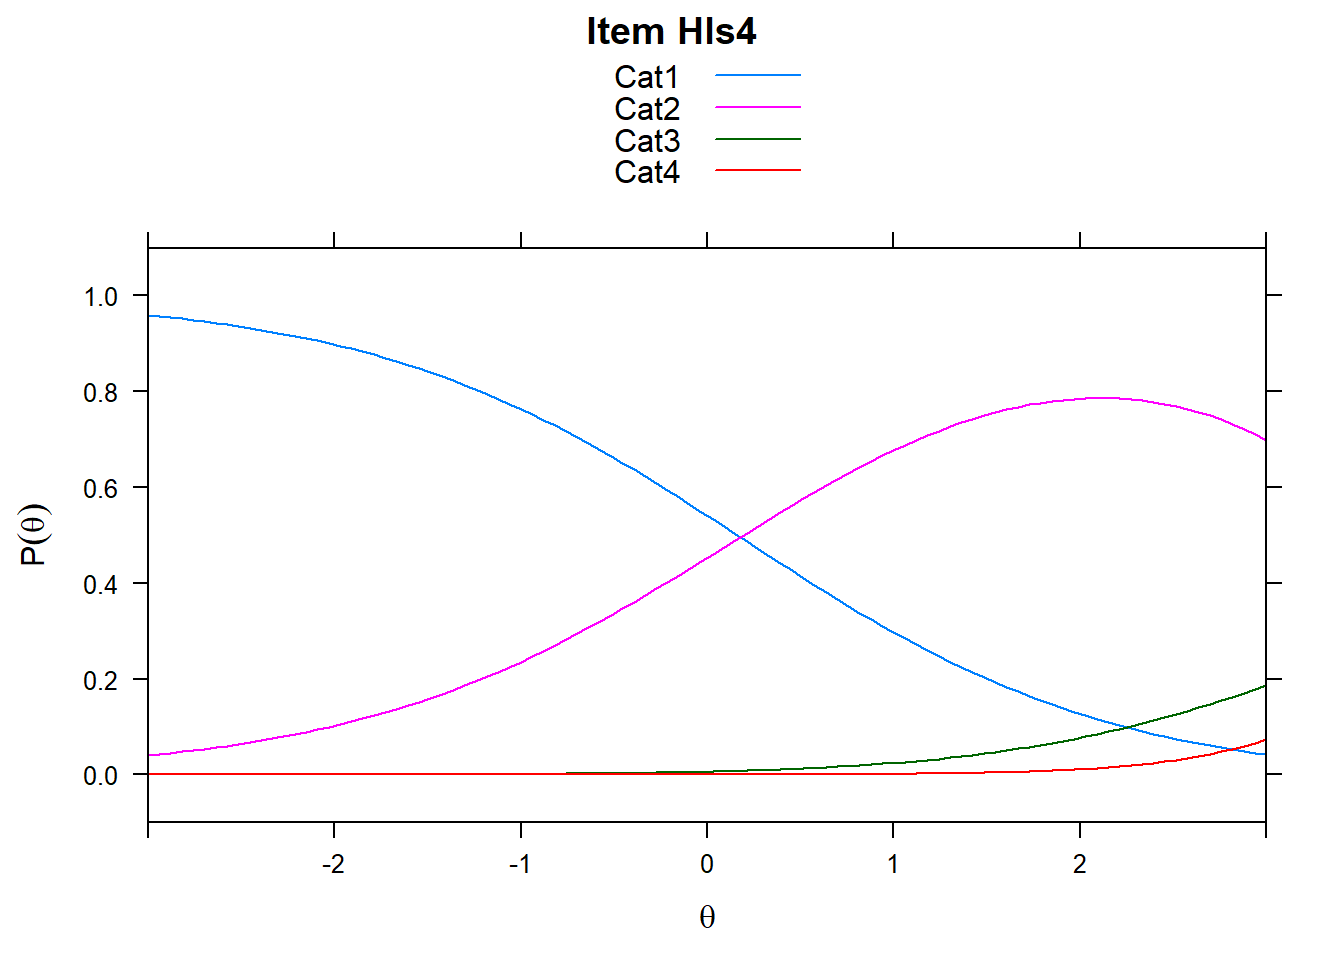
\includegraphics{Rasch_Biome_files/figure-latex/unnamed-chunk-51-4.pdf} 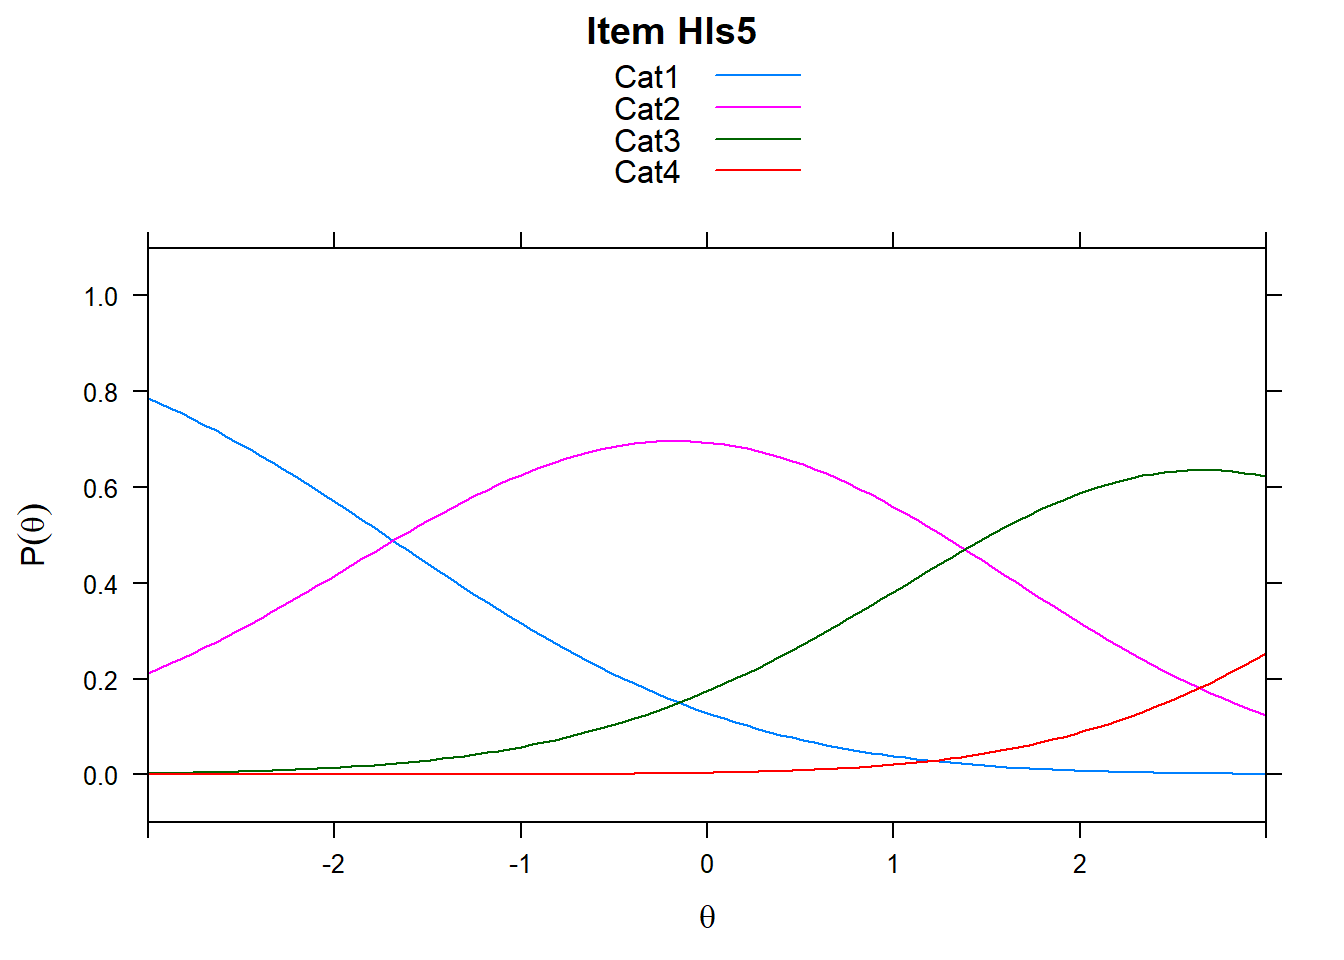
\includegraphics{Rasch_Biome_files/figure-latex/unnamed-chunk-51-5.pdf} 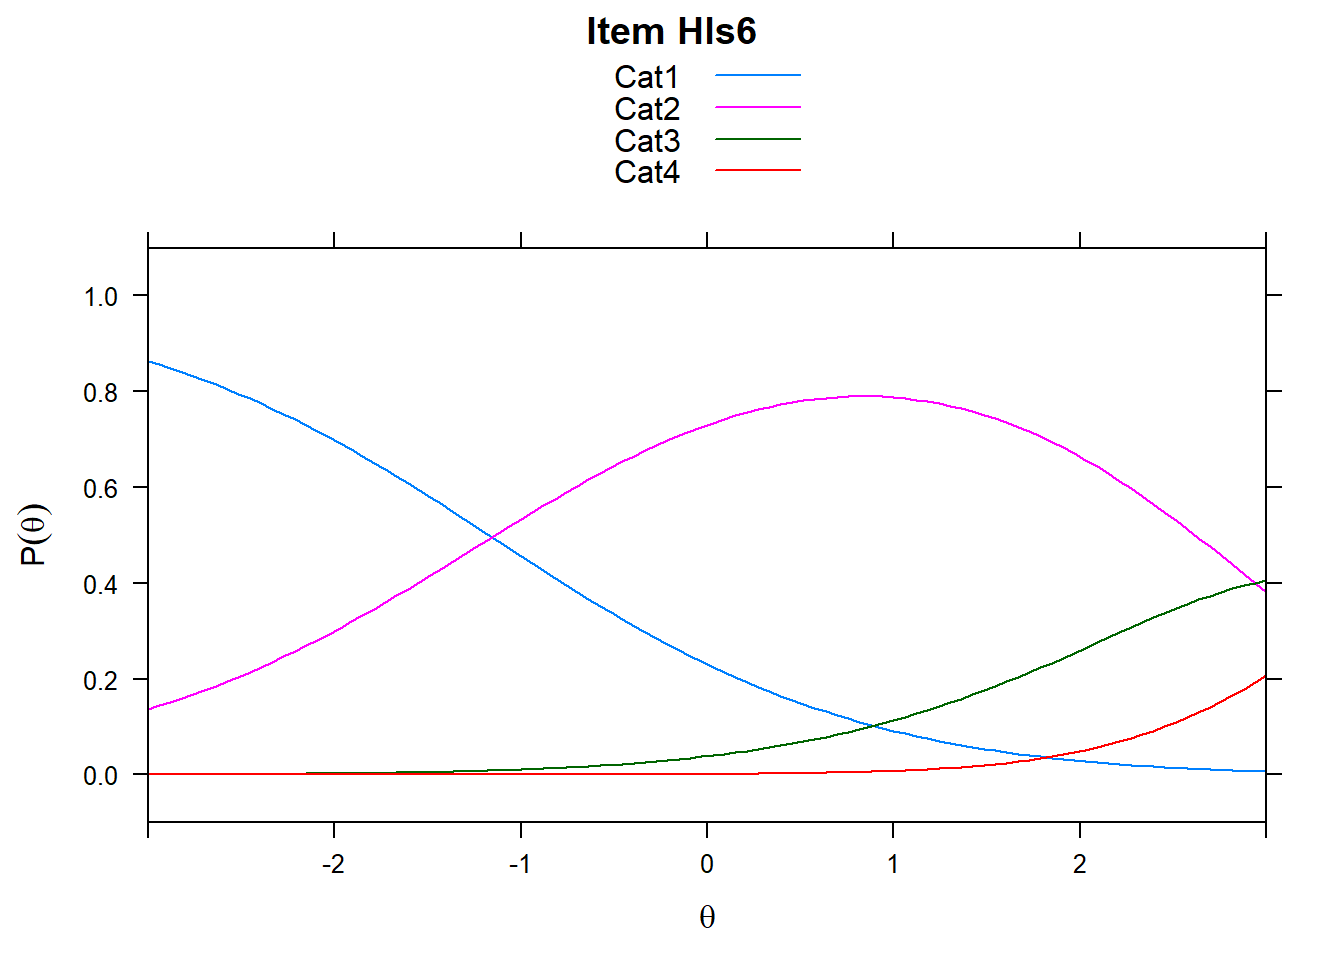
\includegraphics{Rasch_Biome_files/figure-latex/unnamed-chunk-51-6.pdf} 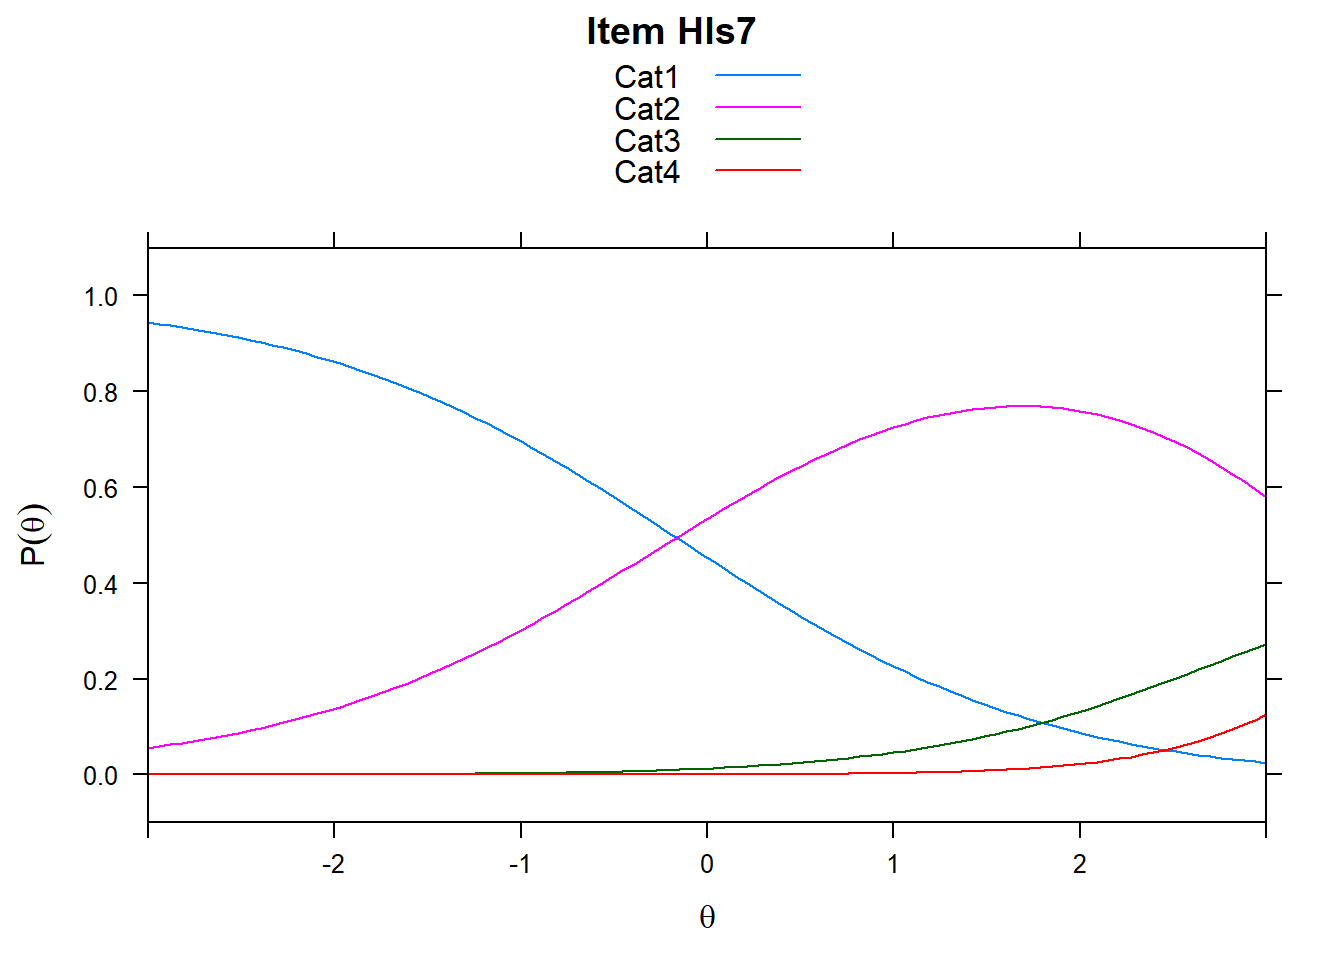
\includegraphics{Rasch_Biome_files/figure-latex/unnamed-chunk-51-7.pdf} 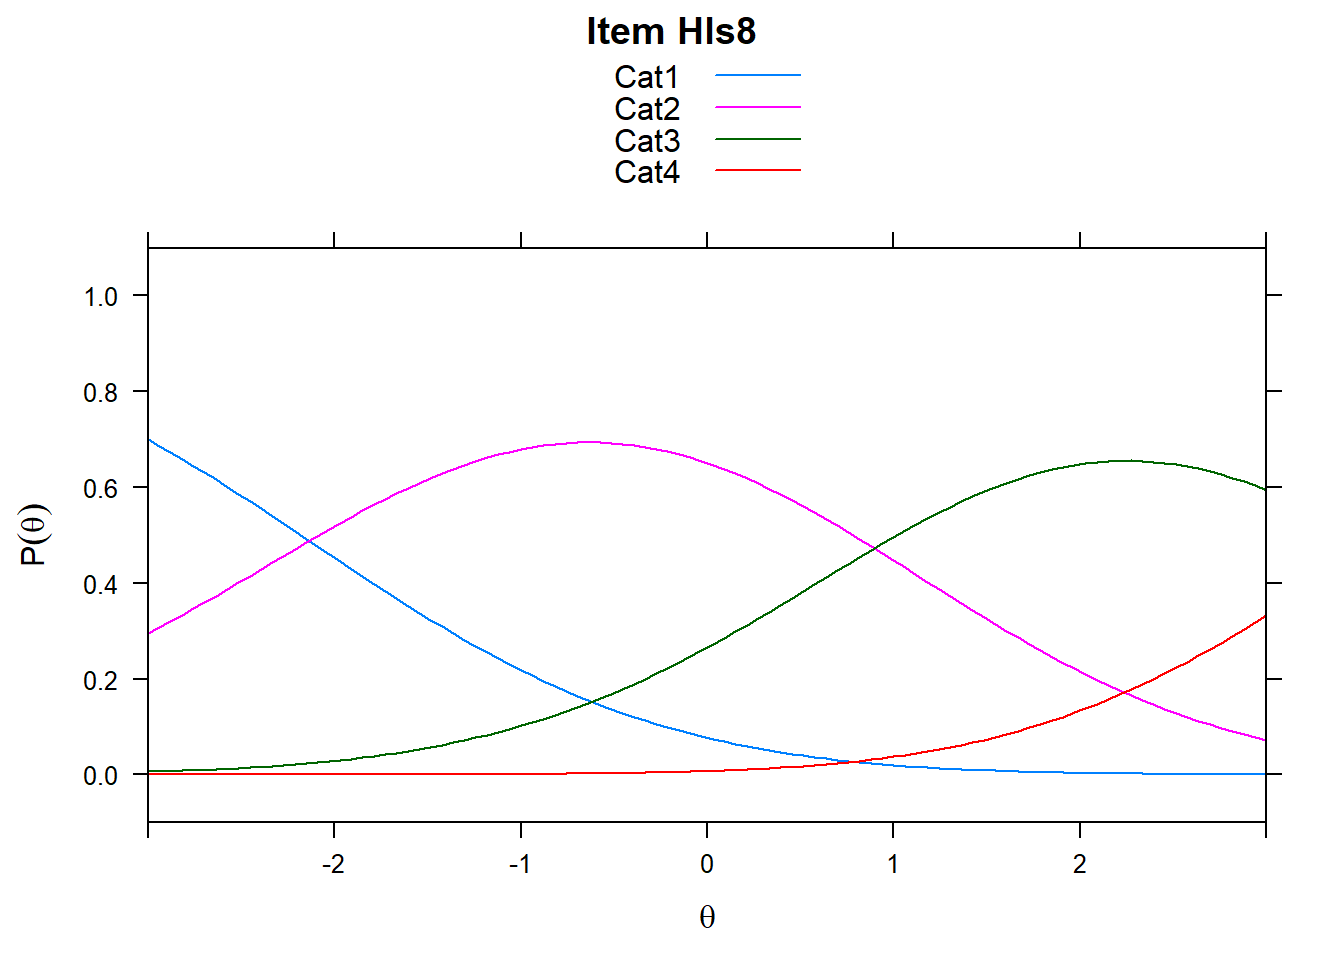
\includegraphics{Rasch_Biome_files/figure-latex/unnamed-chunk-51-8.pdf} 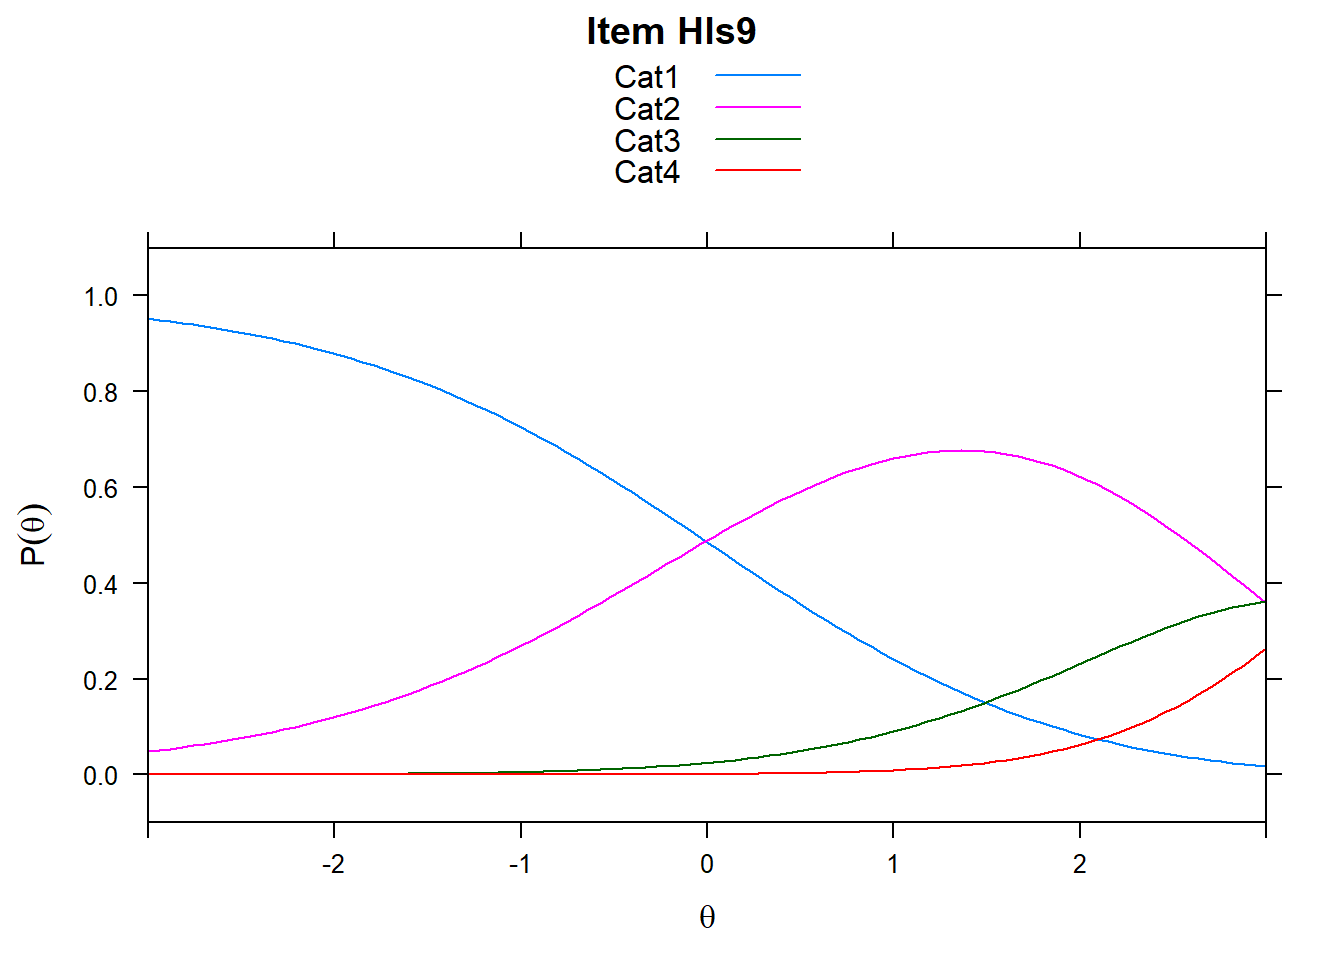
\includegraphics{Rasch_Biome_files/figure-latex/unnamed-chunk-51-9.pdf} 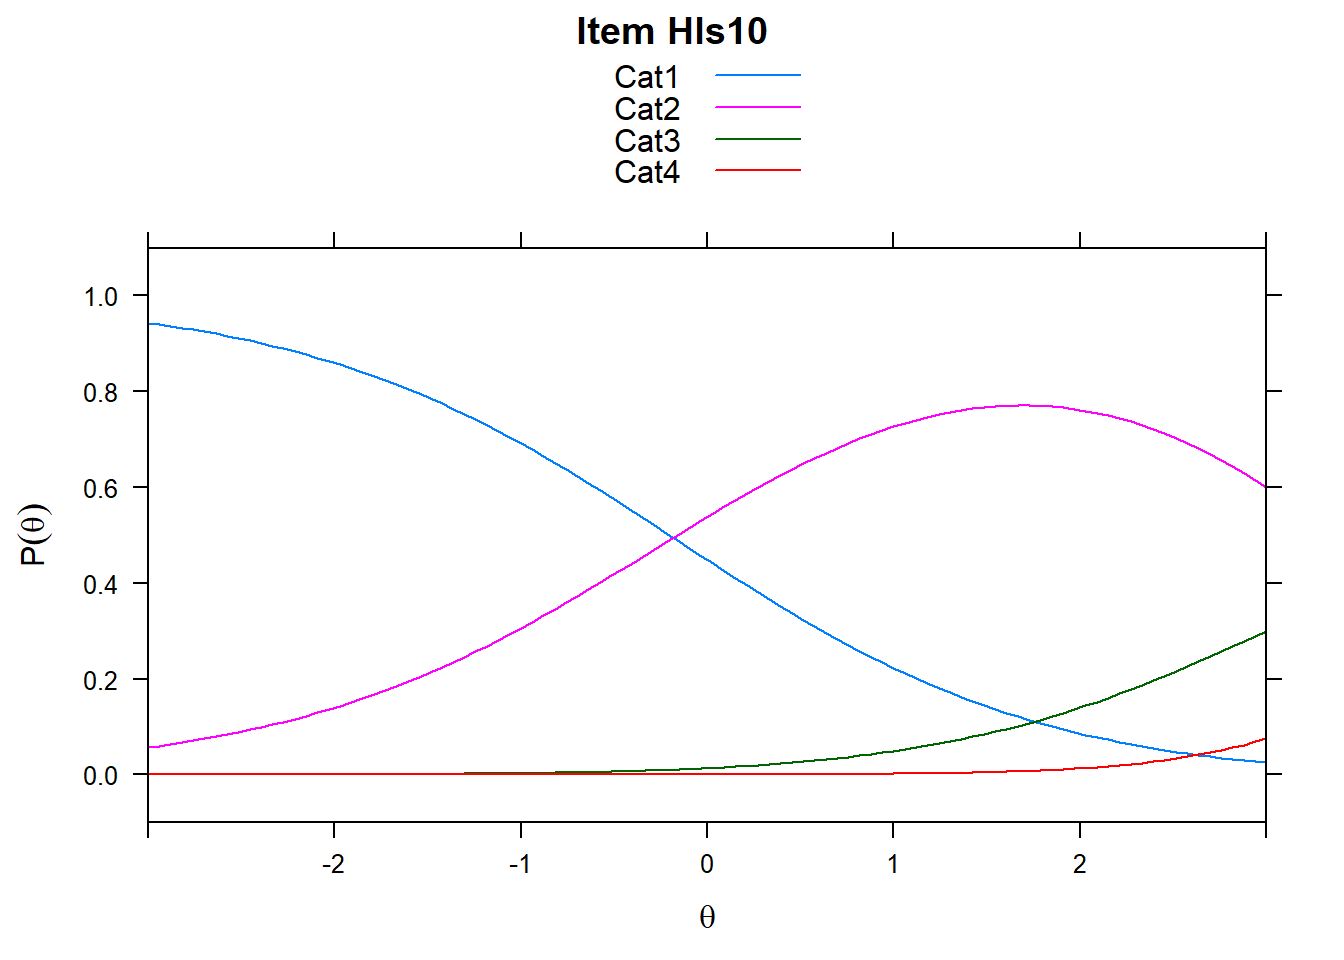
\includegraphics{Rasch_Biome_files/figure-latex/unnamed-chunk-51-10.pdf} 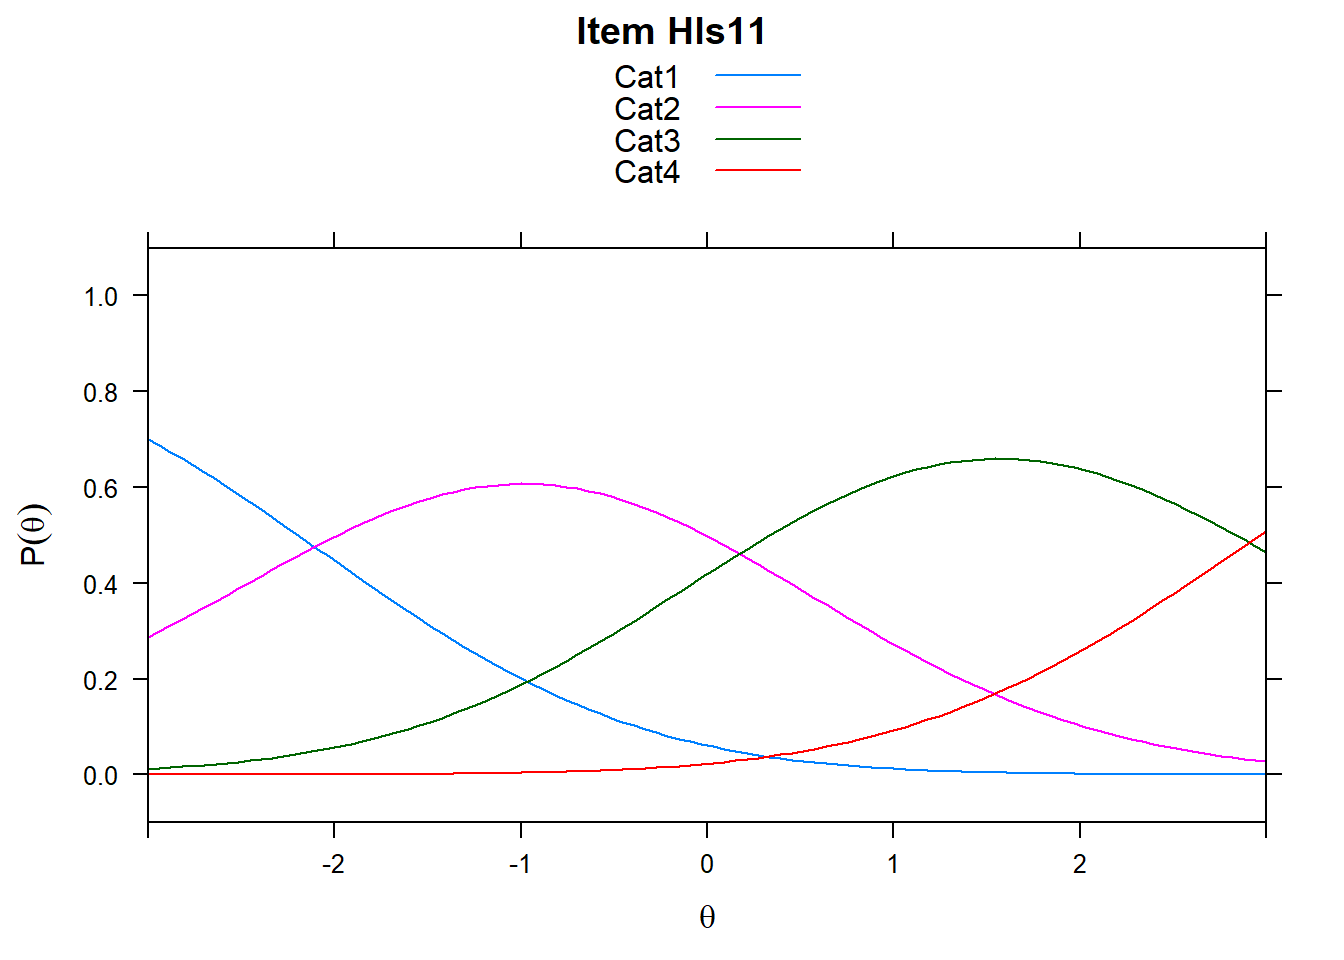
\includegraphics{Rasch_Biome_files/figure-latex/unnamed-chunk-51-11.pdf} 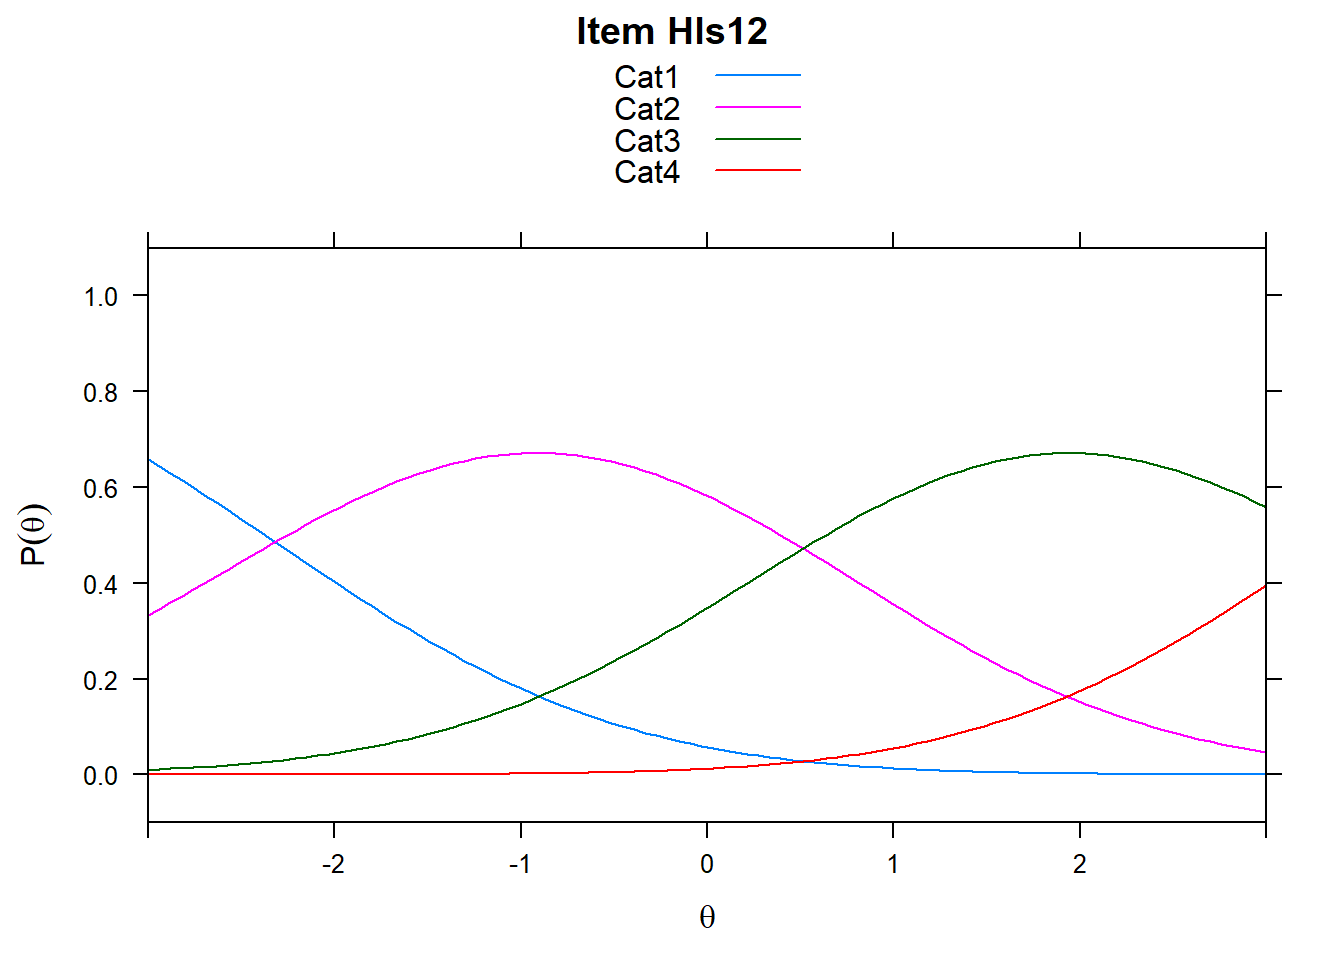
\includegraphics{Rasch_Biome_files/figure-latex/unnamed-chunk-51-12.pdf} 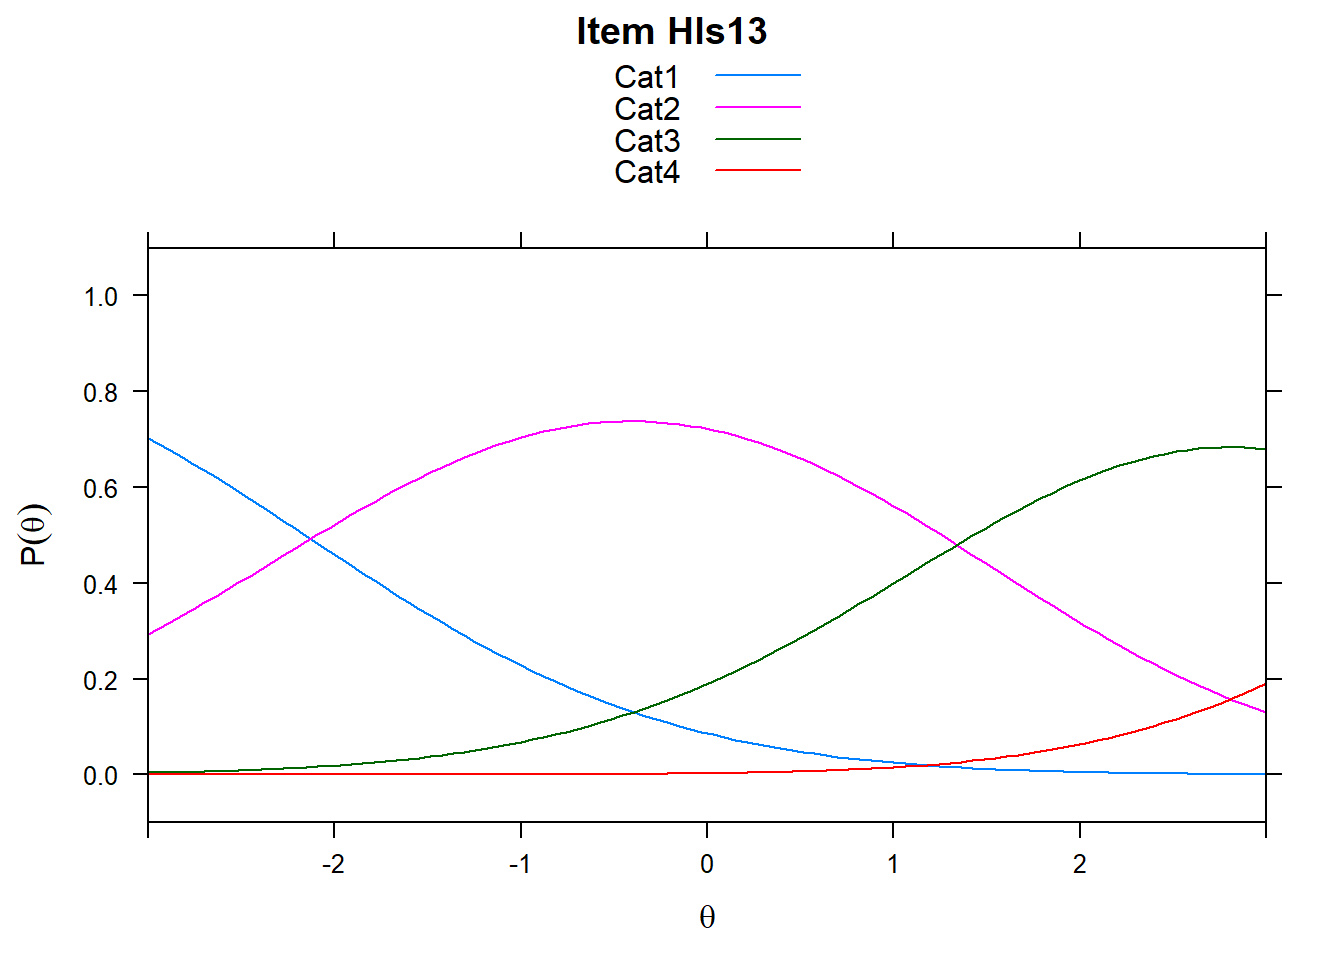
\includegraphics{Rasch_Biome_files/figure-latex/unnamed-chunk-51-13.pdf} 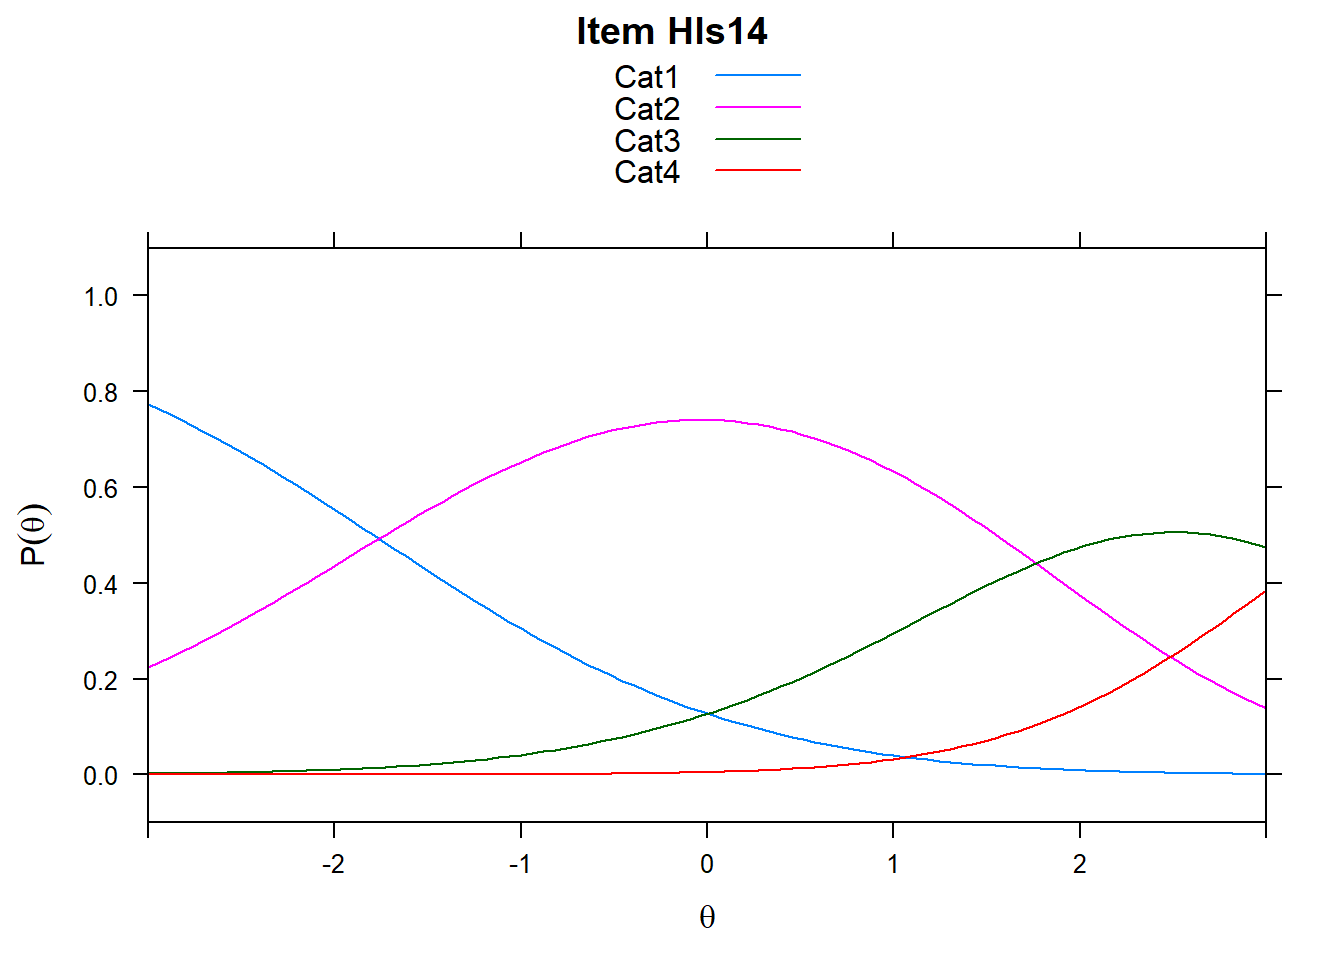
\includegraphics{Rasch_Biome_files/figure-latex/unnamed-chunk-51-14.pdf} 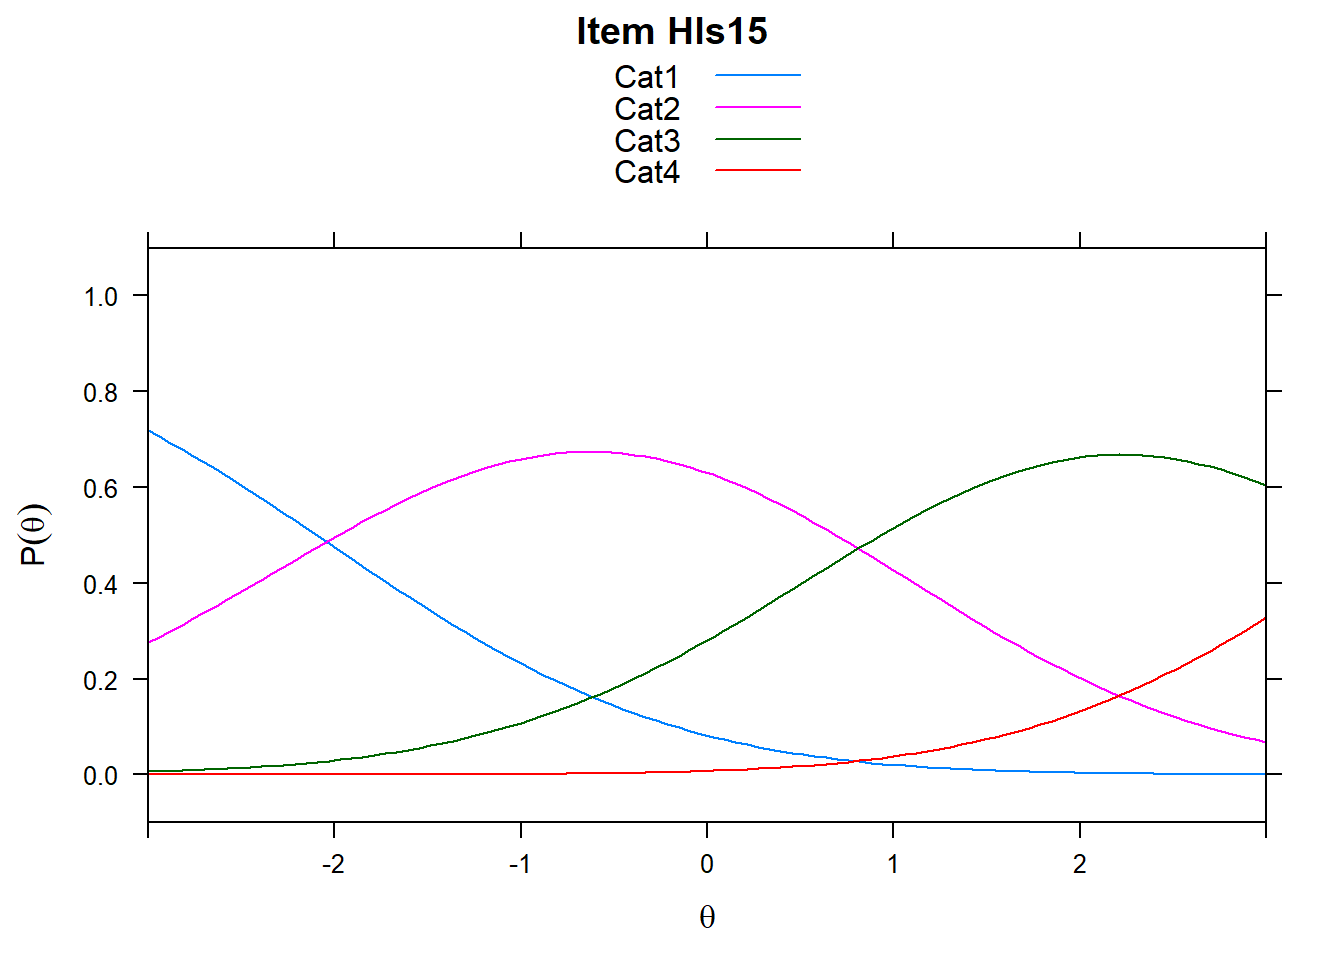
\includegraphics{Rasch_Biome_files/figure-latex/unnamed-chunk-51-15.pdf} 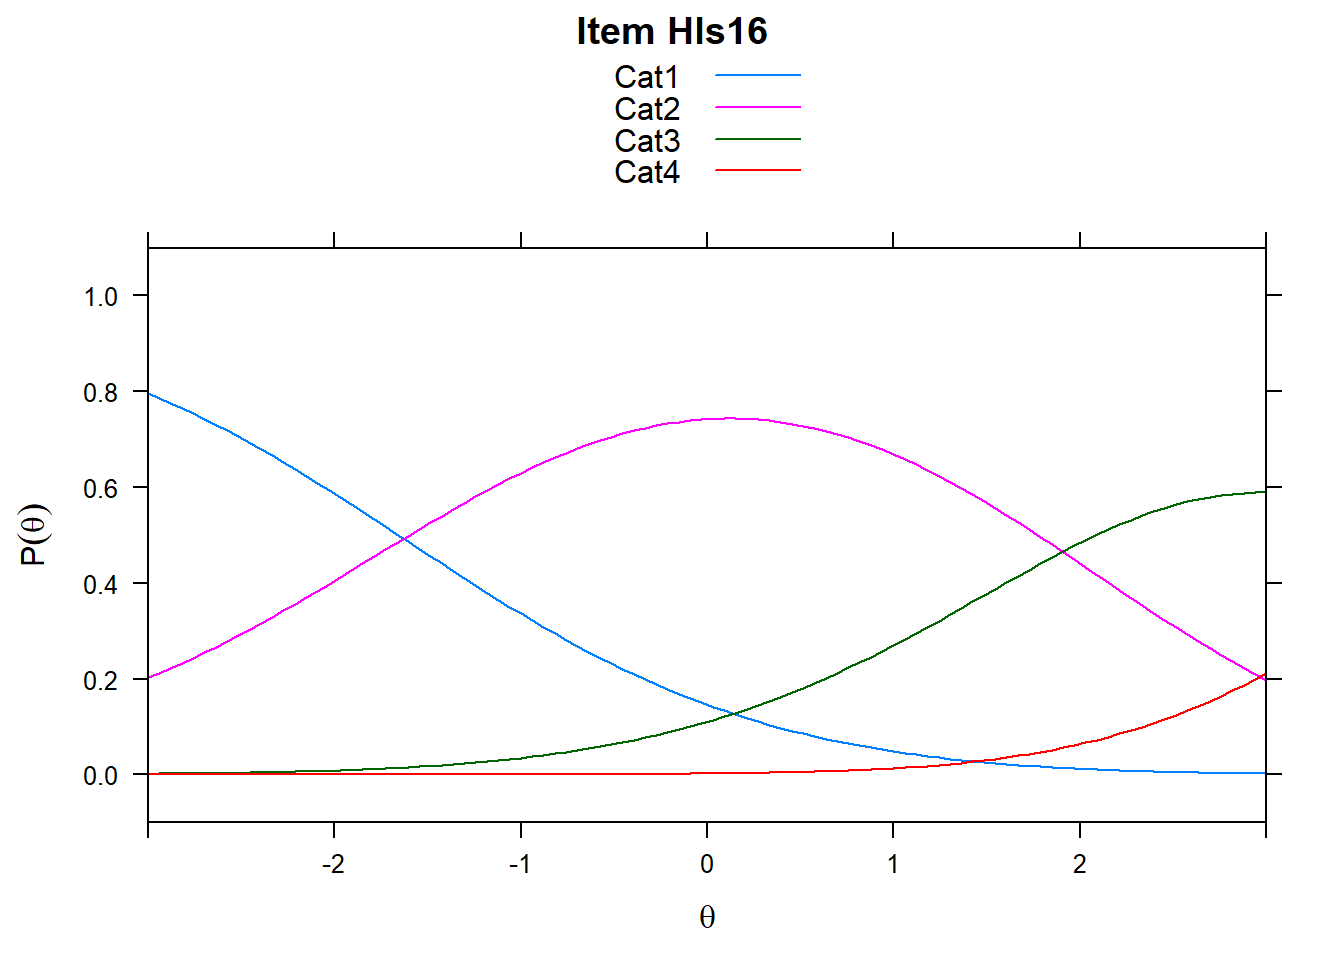
\includegraphics{Rasch_Biome_files/figure-latex/unnamed-chunk-51-16.pdf}

\begin{verbatim}
## ....................................................
##  Plots exported in png format into folder:
##  C:/Users/katzd/Desktop/Rprojects/Rasch_BIOME/DBER_Rasch-data/Plots
\end{verbatim}

\hypertarget{wright-map-1}{%
\section{Wright Map}\label{wright-map-1}}

Here's a polytomous Wright Map

\begin{Shaded}
\begin{Highlighting}[]
\FunctionTok{wrightMap}\NormalTok{(person.ability.poly, tthresh.poly)}
\end{Highlighting}
\end{Shaded}

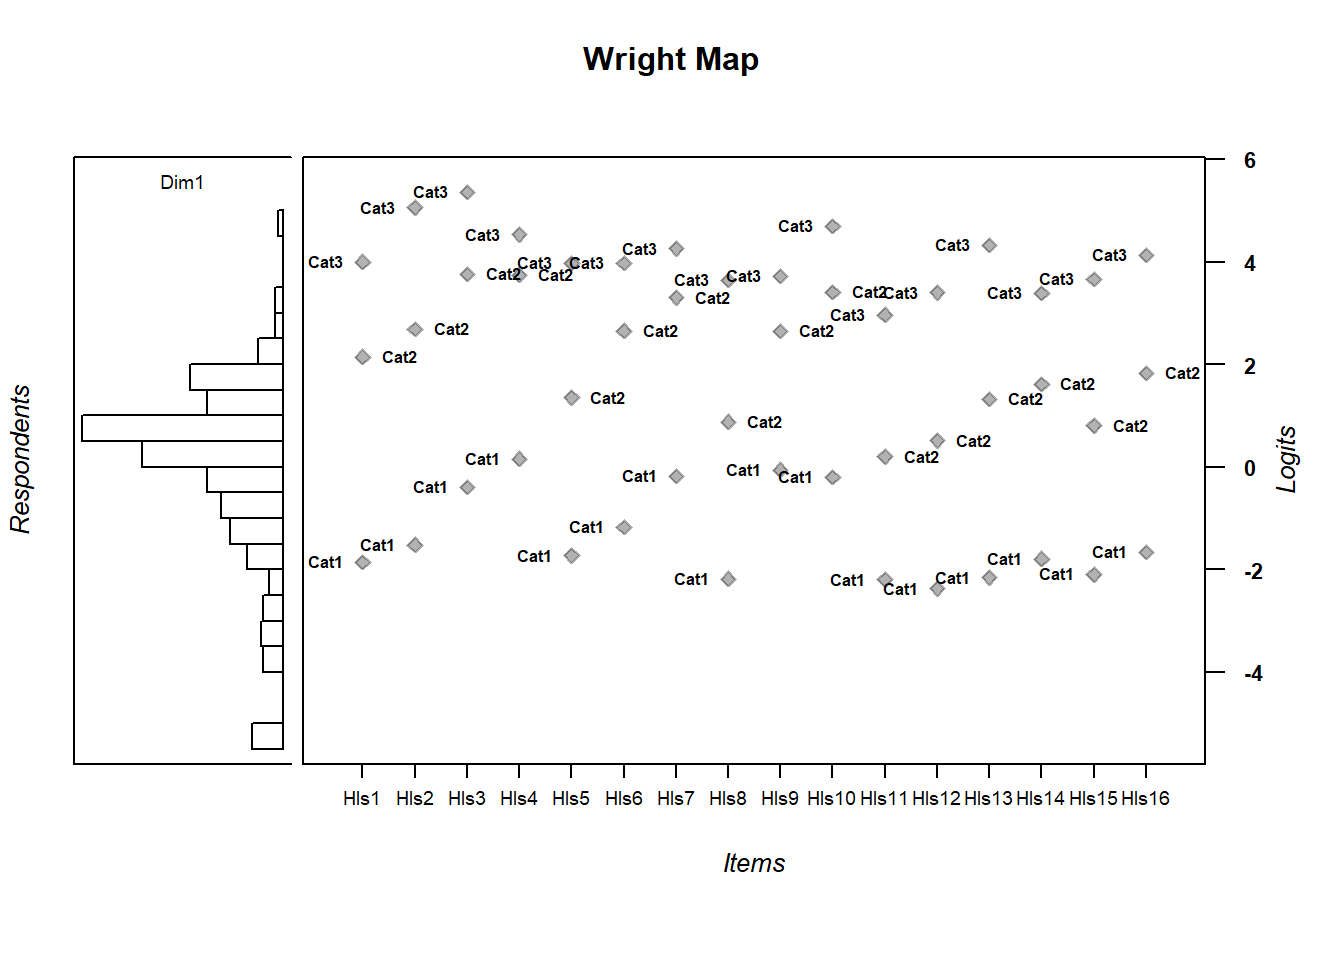
\includegraphics{Rasch_Biome_files/figure-latex/unnamed-chunk-52-1.pdf}

\begin{verbatim}
##              Cat1      Cat2     Cat3
## Hls1  -1.86154175 2.1462708 3.998566
## Hls2  -1.51547241 2.6820374 5.054901
## Hls3  -0.39358521 3.7526550 5.350800
## Hls4   0.16012573 3.7458801 4.529205
## Hls5  -1.72787476 1.3532410 3.970184
## Hls6  -1.17178345 2.6529236 3.976410
## Hls7  -0.18539429 3.3007507 4.254547
## Hls8  -2.18106079 0.8795471 3.643341
## Hls9  -0.05612183 2.6443176 3.715851
## Hls10 -0.20352173 3.4025574 4.694550
## Hls11 -2.19607544 0.2026062 2.966949
## Hls12 -2.37240601 0.5131531 3.396881
## Hls13 -2.15725708 1.3193665 4.324860
## Hls14 -1.78994751 1.6114197 3.388824
## Hls15 -2.09591675 0.8077698 3.664764
## Hls16 -1.65664673 1.8318787 4.128021
\end{verbatim}

\hypertarget{exercises}{%
\section{Exercises:}\label{exercises}}

\begin{enumerate}
\def\labelenumi{\arabic{enumi}.}
\tightlist
\item
  Find an item for which Cat 3 is actually easier than the Cat 2 of another item.
\item
  Find an item that has two categories that are extremely close in severity.
\item
  Look at the ICC for item 14. Describe what is happening with Cat 3.
\end{enumerate}

\hypertarget{model-comparison}{%
\section{Model Comparison}\label{model-comparison}}

say we want to compare the two models we just ran (note, these aren't really comparable since it's a completely different model - not nested data)

\begin{Shaded}
\begin{Highlighting}[]
\FunctionTok{logLik}\NormalTok{(mod1)}
\end{Highlighting}
\end{Shaded}

\begin{verbatim}
## 'log Lik.' -7343.562 (df=16)
\end{verbatim}

\begin{Shaded}
\begin{Highlighting}[]
\FunctionTok{logLik}\NormalTok{(mod2)}
\end{Highlighting}
\end{Shaded}

\begin{verbatim}
## 'log Lik.' -4185.626 (df=49)
\end{verbatim}

\begin{Shaded}
\begin{Highlighting}[]
\FunctionTok{anova}\NormalTok{(mod1, mod2)}
\end{Highlighting}
\end{Shaded}

\begin{verbatim}
##   Model   loglike  Deviance Npars       AIC       BIC
## 1  mod1 -7343.562 14687.124    16 14719.124 14797.649
## 2  mod2 -4185.626  8371.252    49  8469.252  8653.438
##      Chisq df  p
## 1 6315.872 33  0
## 2       NA NA NA
\end{verbatim}

Log likelihood is the foundation of both AIC and BIC. AIC and BIC allow you to compare non-nested models while penalizing for model complexity (BIC penalizes more). In general, the model with a smaller AIC/BIC is the one that the data fit better. The two criteria sometimes disagree.

\hypertarget{multidimensional}{%
\chapter{Multidimensional Rasch Model}\label{multidimensional}}

What if we envision something that's multidimensional? We can model that with TAM. IN fact, this is one of TAM's great strengths. Do read package documentation, though. As the number of dimensions grows, you'll have to use particular estimation methods else the model will take to long to run.

\hypertarget{we-start-by-assigning-the-items-to-a-dimension-using-a-q-matrix}{%
\section{we start by assigning the items to a dimension using a Q-matrix}\label{we-start-by-assigning-the-items-to-a-dimension-using-a-q-matrix}}

If we want to have two dimensions, we'll create a matrix with two columns. A 1 or 0 denotes whether that item belongs to dimension 1 or 2 (or both!)

\begin{Shaded}
\begin{Highlighting}[]
\NormalTok{Q }\OtherTok{\textless{}{-}} \FunctionTok{matrix}\NormalTok{(}\AttributeTok{data=}\DecValTok{0}\NormalTok{, }\AttributeTok{nrow=}\DecValTok{15}\NormalTok{, }\AttributeTok{ncol=}\DecValTok{2}\NormalTok{)}

\NormalTok{Q[}\DecValTok{1}\SpecialCharTok{:}\DecValTok{7}\NormalTok{, }\DecValTok{1}\NormalTok{] }\OtherTok{\textless{}{-}}\DecValTok{1}
\NormalTok{Q[}\DecValTok{8}\SpecialCharTok{:}\DecValTok{15}\NormalTok{, }\DecValTok{2}\NormalTok{] }\OtherTok{\textless{}{-}} \DecValTok{1}




\NormalTok{Q}
\end{Highlighting}
\end{Shaded}

\begin{verbatim}
##       [,1] [,2]
##  [1,]    1    0
##  [2,]    1    0
##  [3,]    1    0
##  [4,]    1    0
##  [5,]    1    0
##  [6,]    1    0
##  [7,]    1    0
##  [8,]    0    1
##  [9,]    0    1
## [10,]    0    1
## [11,]    0    1
## [12,]    0    1
## [13,]    0    1
## [14,]    0    1
## [15,]    0    1
\end{verbatim}

click on the ``Q'' object in the environment pane to see what we just made

\hypertarget{run-the-multidimensional-rasch-model}{%
\section{Run the multidimensional Rasch model}\label{run-the-multidimensional-rasch-model}}

\begin{Shaded}
\begin{Highlighting}[]
\NormalTok{multi }\OtherTok{\textless{}{-}}\NormalTok{ TAM}\SpecialCharTok{::}\FunctionTok{tam.mml}\NormalTok{(}\AttributeTok{resp=}\NormalTok{hls, }\AttributeTok{Q=}\NormalTok{Q)}
\end{Highlighting}
\end{Shaded}

\hypertarget{theta-and-delta}{%
\section{\texorpdfstring{\(\theta\) and \(\delta\)}{\textbackslash theta and \textbackslash delta}}\label{theta-and-delta}}

\begin{Shaded}
\begin{Highlighting}[]
\NormalTok{persons.multi }\OtherTok{\textless{}{-}} \FunctionTok{tam.wle}\NormalTok{(multi)}
\end{Highlighting}
\end{Shaded}

\begin{verbatim}
## Iteration in WLE/MLE estimation  1   | Maximal change  2.105 
## Iteration in WLE/MLE estimation  2   | Maximal change  0.7201 
## Iteration in WLE/MLE estimation  3   | Maximal change  0.0844 
## Iteration in WLE/MLE estimation  4   | Maximal change  0.0235 
## Iteration in WLE/MLE estimation  5   | Maximal change  0.0077 
## Iteration in WLE/MLE estimation  6   | Maximal change  0.0026 
## Iteration in WLE/MLE estimation  7   | Maximal change  9e-04 
## Iteration in WLE/MLE estimation  8   | Maximal change  3e-04 
## Iteration in WLE/MLE estimation  9   | Maximal change  1e-04 
## 
## -------
## WLE Reliability (Dimension1)=0.185 
## WLE Reliability (Dimension2)=0.492
\end{verbatim}

\begin{Shaded}
\begin{Highlighting}[]
\NormalTok{WLEestimates.multi }\OtherTok{\textless{}{-}}\NormalTok{ persons.multi}\SpecialCharTok{$}\NormalTok{theta}
\NormalTok{thresholds.multi }\OtherTok{\textless{}{-}} \FunctionTok{tam.threshold}\NormalTok{(multi)}
\end{Highlighting}
\end{Shaded}

\begin{Shaded}
\begin{Highlighting}[]
\CommentTok{\#Fit and reliabilities}
\NormalTok{Fit.multi }\OtherTok{\textless{}{-}} \FunctionTok{tam.fit}\NormalTok{(multi)}
\end{Highlighting}
\end{Shaded}

\begin{verbatim}
## Item fit calculation based on 15 simulations
## |**********|
## |----------|
\end{verbatim}

\begin{Shaded}
\begin{Highlighting}[]
\NormalTok{Fit.multi}\SpecialCharTok{$}\NormalTok{itemfit}
\end{Highlighting}
\end{Shaded}

\begin{verbatim}
##    parameter    Outfit   Outfit_t     Outfit_p Outfit_pholm
## 1         V1 0.6556239 -7.7047951 1.310534e-14 1.834748e-13
## 2         V2 3.5585941 16.4958991 3.926711e-61 5.890066e-60
## 3         V3 1.0123342  0.2359310 8.134862e-01 1.000000e+00
## 4         V4 0.9327988 -1.2449594 2.131467e-01 1.000000e+00
## 5         V5 1.0276519  0.7548666 4.503290e-01 1.000000e+00
## 6         V6 0.9906337 -0.3611783 7.179662e-01 1.000000e+00
## 7         V7 0.9499635 -1.9123890 5.582632e-02 7.257421e-01
## 8         V8 0.9796108 -0.7795409 4.356612e-01 1.000000e+00
## 9         V9 0.9964664 -0.1438517 8.856176e-01 1.000000e+00
## 10       V10 1.0230307  0.2659752 7.902583e-01 1.000000e+00
## 11       V11 0.9373510 -0.9415633 3.464163e-01 1.000000e+00
## 12       V12 1.0415319  0.9988421 3.178712e-01 1.000000e+00
## 13       V13 0.8596629 -1.3838661 1.663995e-01 1.000000e+00
## 14       V14 0.9559039 -1.5642784 1.177522e-01 1.000000e+00
## 15       V15 0.9900436 -0.3813642 7.029330e-01 1.000000e+00
##        Infit    Infit_t      Infit_p Infit_pholm
## 1  0.8351894 -3.4080972 0.0006541759 0.009812638
## 2  1.2379608  2.3364192 0.0194694053 0.272571674
## 3  1.0301864  0.5800003 0.5619144280 1.000000000
## 4  0.9707091 -0.5214016 0.6020870023 1.000000000
## 5  1.0236420  0.6538801 0.5131890529 1.000000000
## 6  0.9968850 -0.1202964 0.9042483307 1.000000000
## 7  0.9720519 -1.0567134 0.2906424220 1.000000000
## 8  0.9756781 -0.9219008 0.3565803162 1.000000000
## 9  0.9864472 -0.5038357 0.6143768053 1.000000000
## 10 0.9990221  0.0152187 0.9878577018 1.000000000
## 11 0.9874540 -0.1661856 0.8680108531 1.000000000
## 12 1.0218284  0.5378474 0.5906824003 1.000000000
## 13 1.0101894  0.1270731 0.8988825349 1.000000000
## 14 0.9692592 -1.0795983 0.2803210945 1.000000000
## 15 0.9935456 -0.2425653 0.8083421694 1.000000000
\end{verbatim}

\begin{Shaded}
\begin{Highlighting}[]
\NormalTok{multi}\SpecialCharTok{$}\NormalTok{EAP.rel }\CommentTok{\#EAP reliabilities}
\end{Highlighting}
\end{Shaded}

\begin{verbatim}
##      Dim1      Dim2 
## 0.6738227 0.6814934
\end{verbatim}

\hypertarget{wright-map-2}{%
\subsection{Wright Map}\label{wright-map-2}}

\begin{Shaded}
\begin{Highlighting}[]
\NormalTok{MDthetas.multi }\OtherTok{\textless{}{-}}
  \FunctionTok{cbind}\NormalTok{(persons.multi}\SpecialCharTok{$}\NormalTok{theta.Dim01,persons.multi}\SpecialCharTok{$}\NormalTok{theta.Dim02) }\CommentTok{\#one line}
\FunctionTok{wrightMap}\NormalTok{(MDthetas.multi, thresholds.multi) }\CommentTok{\#second line}
\end{Highlighting}
\end{Shaded}

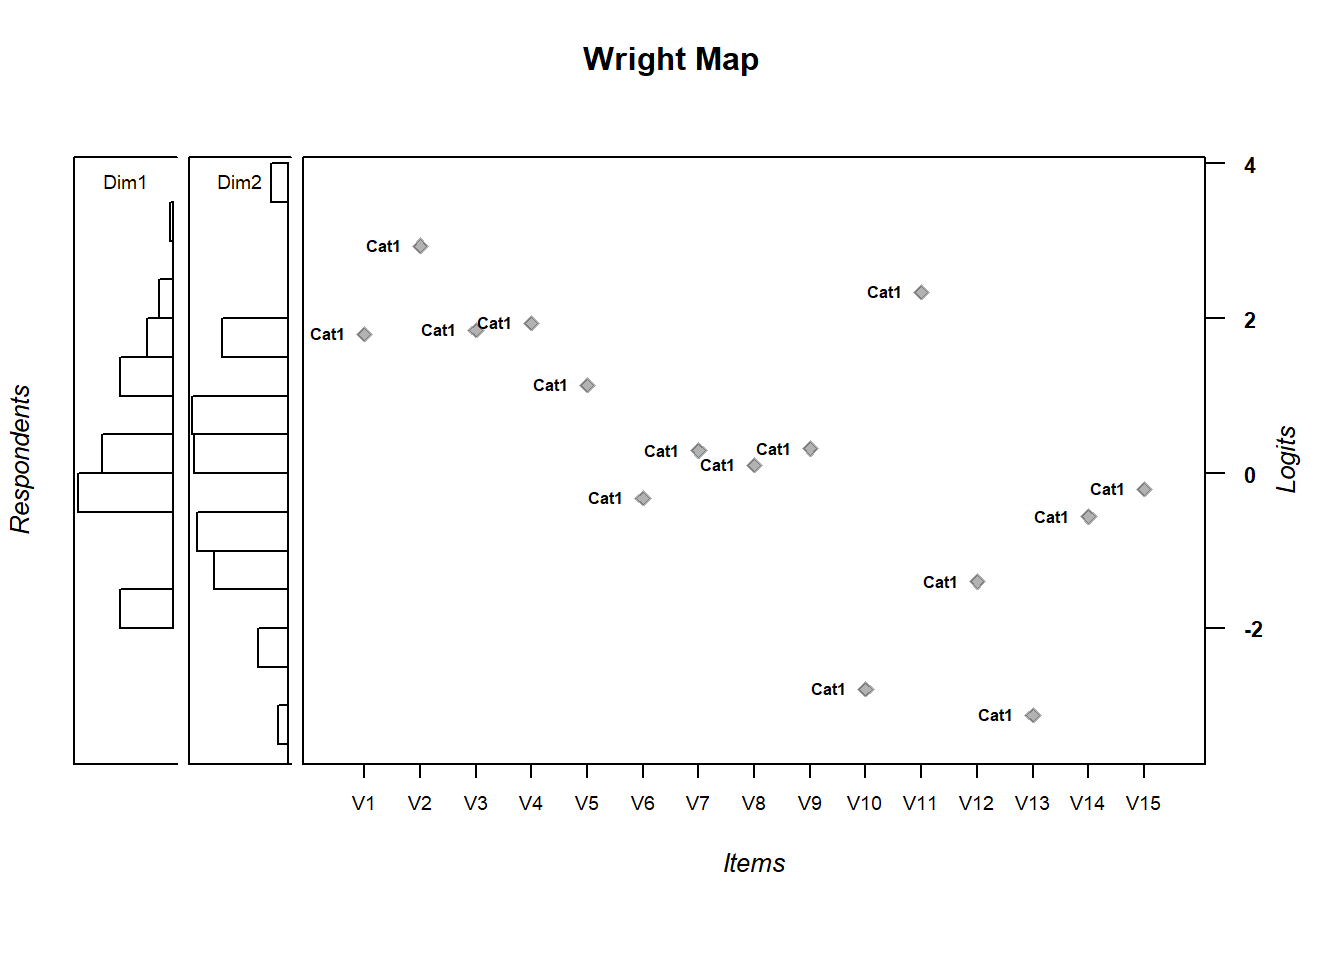
\includegraphics{Rasch_Biome_files/figure-latex/unnamed-chunk-59-1.pdf}

\begin{verbatim}
##           Cat1
## V1   1.7928772
## V2   2.9363708
## V3   1.8478088
## V4   1.9375305
## V5   1.1390076
## V6  -0.3249207
## V7   0.2915955
## V8   0.1009827
## V9   0.3188782
## V10 -2.7882385
## V11  2.3348694
## V12 -1.3975525
## V13 -3.1209412
## V14 -0.5602112
## V15 -0.2038879
\end{verbatim}

Compare the first unidimensional model to the multidimensional one

\begin{Shaded}
\begin{Highlighting}[]
\FunctionTok{logLik}\NormalTok{(mod1)}
\end{Highlighting}
\end{Shaded}

\begin{verbatim}
## 'log Lik.' -7343.562 (df=16)
\end{verbatim}

\begin{Shaded}
\begin{Highlighting}[]
\FunctionTok{logLik}\NormalTok{(multi)}
\end{Highlighting}
\end{Shaded}

\begin{verbatim}
## 'log Lik.' -7334.79 (df=18)
\end{verbatim}

\begin{Shaded}
\begin{Highlighting}[]
\FunctionTok{anova}\NormalTok{(mod1, multi)}
\end{Highlighting}
\end{Shaded}

\begin{verbatim}
##   Model   loglike Deviance Npars      AIC      BIC    Chisq
## 1  mod1 -7343.562 14687.12    16 14719.12 14797.65 17.54463
## 2 multi -7334.790 14669.58    18 14705.58 14793.92       NA
##   df       p
## 1  2 0.00015
## 2 NA      NA
\end{verbatim}

Alternatively, you can use \texttt{IRT.compareModels}

\begin{Shaded}
\begin{Highlighting}[]
\NormalTok{compare }\OtherTok{\textless{}{-}}\NormalTok{ CDM}\SpecialCharTok{::}\FunctionTok{IRT.compareModels}\NormalTok{(mod1, multi)}
\NormalTok{compare}
\end{Highlighting}
\end{Shaded}

\begin{verbatim}
## $IC
##   Model   loglike Deviance Npars Nobs      AIC      BIC
## 1  mod1 -7343.562 14687.12    16 1000 14719.12 14797.65
## 2 multi -7334.790 14669.58    18 1000 14705.58 14793.92
##       AIC3     AICc     CAIC
## 1 14735.12 14719.68 14813.65
## 2 14723.58 14706.28 14811.92
## 
## $LRtest
##   Model1 Model2     Chi2 df            p
## 1   mod1  multi 17.54463  2 0.0001549648
## 
## attr(,"class")
## [1] "IRT.compareModels"
\end{verbatim}

\begin{Shaded}
\begin{Highlighting}[]
\FunctionTok{summary}\NormalTok{(compare)}
\end{Highlighting}
\end{Shaded}

\begin{verbatim}
## Absolute and relative model fit
## 
##   Model   loglike Deviance Npars Nobs      AIC      BIC
## 1  mod1 -7343.562 14687.12    16 1000 14719.12 14797.65
## 2 multi -7334.790 14669.58    18 1000 14705.58 14793.92
##       AIC3     AICc     CAIC
## 1 14735.12 14719.68 14813.65
## 2 14723.58 14706.28 14811.92
## 
## Likelihood ratio tests - model comparison 
## 
##   Model1 Model2    Chi2 df     p
## 1   mod1  multi 17.5446  2 2e-04
\end{verbatim}

We see that model \texttt{multi} fits slightly better. However, the log likelihood difference test shows the difference is statististically significant.

\begin{tabular}{l|l|r|r|r}
\hline
Model1 & Model2 & Chi2 & df & p\\
\hline
mod1 & multi & 17.54463 & 2 & 0.000155\\
\hline
\end{tabular}

\begin{verbatim}
compare$LRtest
\end{verbatim}

\hypertarget{exercises-1}{%
\section{Exercises}\label{exercises-1}}

\begin{enumerate}
\def\labelenumi{\arabic{enumi}.}
\tightlist
\item
  what evidence points towards multidimensionality?
\item
  compare the multidimensional model to the PCM model
\end{enumerate}

  \bibliography{ref.bib}

\end{document}
